% (c) 2012 -2014 Dimitrios Vrettos - d.vrettos@gmail.com
% (c) 2012 Claudio Carboncini - claudio.carboncini@gmail.com
\chapter{Frazioni e numeri razionali}
\section{Premessa storica}

Quando si deve dividere una certa grandezza o totalità in un certo numero di parti uguali non sempre
sono sufficienti i numeri interi per rappresentare il risultato della divisione. Per esempio, per dividere
l'unità in due parti uguali i numeri interi non sono sufficienti.

Gli antichi hanno affrontato questo tipo di problema utilizzando varie scritture per rappresentare
le parti in cui dividere l'unità, ossia le frazioni.

I Babilonesi scrivevano frazioni aventi come denominatore una potenza di~60, la base della
loro numerazione; tuttavia non usavano una notazione specifica per le frazioni ed
il valore corretto andava interpretato dal contesto.

Gli Egizi facevano largo uso dei numeri frazionari che rappresentavano come somme di frazioni unitarie,
ossia frazioni con numeratore uno. La frazione unitaria~$\frac{1}{n}$ 
veniva rappresentata in forma geroglifica ponendo il denominatore~$n$ scritto con la normale rappresentazione del numero~$n$ sotto ad un ovale. La frazione~$\frac{1}{12}$, per esempio, veniva così rappresentata:

\begin{center}
 % (c) 2012 Dimitrios Vrettos - d.vrettos@gmail.com
    \begin{hieroglyph}{\leavevmode \Cadrat{\CadratLineI{\Aca GD/52/}\CadratLine{\Aca GV/51/\hfill\Aca GZ/32/\hfill\Aca GZ/32/}}}\end{hieroglyph}

\end{center}

Nel ``papiro di Ahmes'' (detto anche ``papiro di Rhind''\footnote{\url{http://it.wikipedia.org/wiki/Papiro_di_Rhind}}) troviamo una tabella che dà la scomposizione in frazioni
unitarie delle frazioni del tipo~$\frac{2}{n}$, con~$n$ dispari: la frazione~$\frac{2}{43}$
è rappresentata come somma di frazioni
unitarie nel seguente modo:

\[\frac{2}{43}=\frac{1}{42}+\frac{1}{86}+\frac{1}{129}+\frac{1}{301}.\]
\begin{wrapfigure}{r}{0pt}
% (c) 2012 Dimitrios Vrettos - d.vrettos@gmail.com
% Occhio di Horus 
\pgfdeclareimage[interpolate=true]{eye}{./img/part01/chap03/eye.pdf}
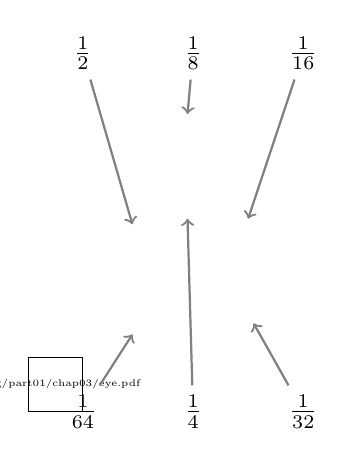
\begin{tikzpicture}[scale=.7]
    \pgftext[at=\pgfpoint {0mm}{0mm},left,base]{\pgfuseimage{eye}}
    \node (a) at (10mm,65mm) {$\frac{1}{2}$};
    \node (b) at (30mm,65mm) {$\frac{1}{8}$};
    \node (c) at (50mm,65mm) {$\frac{1}{16}$};
    \node (d) at (10mm,0mm) {$\frac{1}{64}$};
    \node (e) at (30mm,0mm) {$\frac{1}{4}$};
    \node (f) at (50mm,0mm) {$\frac{1}{32}$};
  \begin{scope}[->,color=gray, thick]
    \draw (a)--(19mm,34mm);
    \draw (b)--(29mm,54mm);
    \draw (c)--(40mm,35mm);
    \draw (d)--(19mm,14mm);
    \draw (e)--(29mm,35mm);
    \draw (f)--(41mm,16mm);
  \end{scope}
\end{tikzpicture}

\end{wrapfigure}

Alcune unità frazionarie più comuni venivano indicate con le parti dell'occhio di Horus (divinità egizia). Secondo la
leggenda, Horus, nella lotta contro lo zio Seth, reo di avergli ucciso il padre,
perse un occhio le cui parti vennero ritrovate e ricomposte dal dio Toth a meno di una piccola parte.

I Romani fecero poco uso dei numeri frazionari; si limitarono a considerare
le parti delle misure in uso che venivano divise in~12, 24, 36, 48, \ldots Avevano
pertanto simboli e nomi particolari per indicare alcune frazioni. \emph{Semis} per
indicare~$\frac{1}{2}$, il cui simbolo era~$S$ oppure~$Z$; \emph{sextans} per indicare~$\frac{1}{6}$, \emph{dracma} per
indicare~$\frac{1}{96}$ e \emph{obolus} per indicare la sesta parte della \emph{dracma}.

Furono gli arabi a introdurre l'attuale scrittura delle
frazioni e i termini \emph{numeratore} e \emph{denominatore}. Tale notazione venne diffusa in Europa
da Leonardo Pisano (Fibonacci)\footnote{matematico italiano (1170 - 1240).} che con il suo ``Liber Abaci'' (1202) scrive e
opera con le frazioni come oggi le conosciamo.

\section{Frazioni}

\begin{definizione}
Una \emph{frazione} è una coppia ordinata di numeri naturali in cui il primo si chiama \emph{numeratore}
e il secondo \emph{denominatore}. Il denominatore deve essere diverso da zero.
\end{definizione}

\begin{center}
 % (c) 2012 Dimitrios Vrettos - d.vrettos@gmail.com
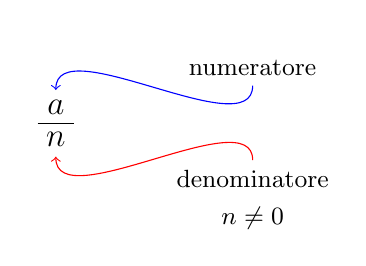
\begin{tikzpicture}
  \begin{scope}[font=\large]
    \matrix (frazione)  at (0,0){%
      \node (num) {$a$};\\
      \node (den) {$n$};\\
    };
  \end{scope}

  \draw (num.south west)--(num.south east);

  \begin{scope}[font=\small]
    \node (testo1) at (25mm,7mm) {numeratore};
    \node (testo2) at (25mm,-7mm) {denominatore};
    \node (testo3) at (25mm,-12mm) {$n\neq0$};
  \end{scope}

  \draw[->,blue] (testo1) .. controls +(down:10mm) and +(up:10mm) .. (num) ;
  \draw[->,red] (testo2) .. controls +(up:10mm) and +(down:10mm) .. (den) ;
\end{tikzpicture}

\end{center}

Quando si chiede, per esempio un quarto di litro di latte,~$\frac{1}{4}\unit{l}$, si danno le informazioni
su come operare sulla grandezza unitaria (litro) per ottenere la quantità desiderata.
Le frazioni possono essere viste come operatori che si applicano a una grandezza fissata, considerata come
l'intero o il tutto, per ottenere una nuova grandezza ben determinata e omogenea alla prima.

Una frazione con numeratore uguale a~1 è detta \emph{frazione unitaria}; indicata con~$A$ una grandezza (segmento, peso,
superficie, angolo, \ldots) la scrittura~$\dfrac{1}{n}A$ sta ad indicare l'operazione di divisione della grandezza~$A$,
intesa come il ``tutto'' (l'intero), in~$n$ parti uguali.

Nella figura seguente, il segmento unitario da~0 a~1 è stato diviso in due parti uguali ottenendo la frazione~$\frac{1}{2}$;
dividendolo in quattro parti uguali si ottiene la frazione~$\frac{1}{4}$;
dividendolo in otto parti uguali si ottiene la frazione~$\frac{1}{8}$;
dividendolo in sedici parti uguali si ottiene la frazione~$\frac{1}{16}$.

\begin{center}
 % (c) 2012 Dimitrios Vrettos - d.vrettos@gmail.com
% 
\begin{tikzpicture}[decoration={markings,mark=between positions 0.7 and .9 step 90pt with {\arrow{stealth}}}]
\begin{scope}[thick]
\draw[->] (0,0) -- (240pt,0);
  \foreach \x/\xtext in {0/0,.5/\frac{1}{16},1/\frac{1}{8},1.5/,2/\frac{1}{4},2.5/,3/,3.5/,4/\frac{1}{2},4.5/,5/,5.5/,6/,6.5/,7/,7.5/,8/1}
    \draw[shift={(\x,0)}] (0pt,2pt) -- (0pt,-2pt) node[below] {$\xtext$};
\end{scope}
\begin{scope}[dotted, color=gray!50!black]
     \draw[postaction={decorate}](0,5pt) arc (180:0:0.25);
     \draw[postaction={decorate}](0,5pt) arc (180:0:0.5);
     \draw[postaction={decorate}](0,5pt) arc (180:0:1);
     \draw[postaction={decorate}](0,5pt) arc (180:0:2);
\end{scope}
\end{tikzpicture}

\end{center}


\osservazione
Il \emph{denominatore} di una frazione è quel numero che indica in quante parti uguali si è diviso l'intero.
Poiché non ha senso dividere un intero in zero parti, il denominatore deve essere diverso da zero.

\begin{wrapfloat}{figure}{r}{0pt}
 % (c) 2012 Dimitrios Vrettos - d.vrettos@gmail.com
% Quadrato 1/4
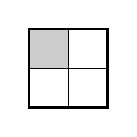
\begin{tikzpicture}
  \begin{scope}[scale=1,every node/.style={minimum size=5mm}]
    \draw[step=5mm, black] (0,0) grid (1,1);
    \fill[gray, opacity=.4] (0,.5) rectangle (.5,1);
    \draw[black,thick] (0,0) rectangle (1,1);
  \end{scope} 
\end{tikzpicture}

\end{wrapfloat}

Vediamo un altro esempio. Il quadrato~$Q$ della figura è stato diviso in quattro parti uguali e
una parte è stata colorata di grigio; questa parte viene indicata con la frazione unitaria~$\dfrac{1}{4}Q$.

L'espressione~$\dfrac{1}{n}A$ significa l'ennesima parte di~$A$, dove~$A$ è il tutto che si deve dividere in~$n$ parti uguali.
In altre parole,
$A$ si può ottenere moltiplicando per~$n$ l'espressione~$\dfrac{1}{n}A$.

Partendo da~$\dfrac{1}{n}A$ si possono considerare i suoi multipli interi:
\[\frac{2}{n}A\text{, }\frac{3}{n}A\text{, }\ldots\text{, }\frac{n}{n}A\] che rappresentano il
doppio di un $n$-esimo di~$A$, il triplo di un $n$-esimo di~$A$, \ldots, l'intera grandezza~$A$.

Riferendoci all'esempio del quadrato ($n=4$):
\begin{center}
 % (c) 2012 Dimitrios Vrettos - d.vrettos@gmail.com
% quadrati e parti di quadrati espresse in frazioni
\begin{tikzpicture}
  \begin{scope}[scale=1,every node/.style={minimum size=5mm}]
    \draw[step=5mm, black] (0,0) grid (1cm,1cm);
    \fill[gray, opacity=.4] (0,.5cm) rectangle (1cm,1cm);
    \draw[black,thick] (0,0) rectangle (1cm,1cm);

    \draw[step=5mm, draw=black, fill=gray] (3cm,0) grid (4cm,1cm);
    \fill[gray, opacity=.4] (3cm,0) rectangle (3.5cm,1cm) ;
    \fill[gray, opacity=.4] (3.5cm,0.5cm)rectangle (4cm,1cm);
    \draw[black,thick] (3cm,0) rectangle (3cm,1cm);

    \draw[step=5mm, draw=black, fill=gray] (6cm,0) grid (7cm,1cm);
    \fill[gray, opacity=.4] (6cm,0) rectangle (7cm,1cm) ;   
    \draw[black,thick] (6cm,0) rectangle (7cm,1cm);
  \end{scope} 
  \node (a) at (1.5cm,.5cm) {$\dfrac{2}{4}Q$};
  \node (b) at (4.5cm,.5cm) {$\dfrac{3}{4}Q$};
  \node (c) at (7.5cm,.5cm) {$\dfrac{4}{4}Q$};
\end{tikzpicture}

\end{center}

La frazione~$\dfrac{m}{n}A$ (si legge \emph{emme ennesimi di}~$A$) indica il multiplo secondo~$m$
della frazione unitaria~$\dfrac{1}{n}A$, cioè la grandezza che si ottiene dividendo~$A$ in~$n$ parti uguali e prendendone~$m$.

\osservazione
 Il \emph{numeratore} di una frazione è quel numero che esprime quante parti, dell'intero suddiviso
in parti uguali secondo il denominatore, devono essere considerate.

Per leggere una frazione si legge prima il numeratore e poi il denominatore.
Quest'ultimo si legge come numero ordinale (terzo/i, quarto/i, quinto/i, \ldots).
Nel caso in cui sia 2 si legge ``mezzo/i''.

\begin{exrig}
\begin{esempio}
 Lettura di frazioni.
 \begin{multicols}{3}
 \begin{enumeratea}
\item $\dfrac{1}{2}$ è un mezzo;
\item $\dfrac{1}{10}$ è un decimo;
\item $\dfrac{2}{3}$ è due terzi;
\item $\dfrac{3}{11}$ è tre undicesimi;
\item $\dfrac{5}{7}$ è cinque settimi;
\item $\dfrac{1}{12}$ è un dodicesimo.
\end{enumeratea}
\end{multicols}
\end{esempio}
\end{exrig}

Per esprimere le frazioni si utilizza anche la scrittura del tipo~$a/b$; es.~$2/3$, $4/6$, $6/9$, \ldots

 \ovalbox{\risolvii \ref{ese:3.1}, \ref{ese:3.2}, \ref{ese:3.3}, \ref{ese:3.4}}

\begin{definizione}
Si chiamano \emph{proprie} le frazioni che hanno il numeratore minore del denominatore.
Esse rappresentano sempre una grandezza minore dell'intero.
\end{definizione}

\pagebreak

Vi sono frazioni che pur essendo formate da numeratori e denominatori diversi rappresentano
la stessa parte dell'intero.
\begin{center}
 % (c) 2012 Dimitrios Vrettos - d.vrettos@gmail.com
% Parti uguali dell'intero
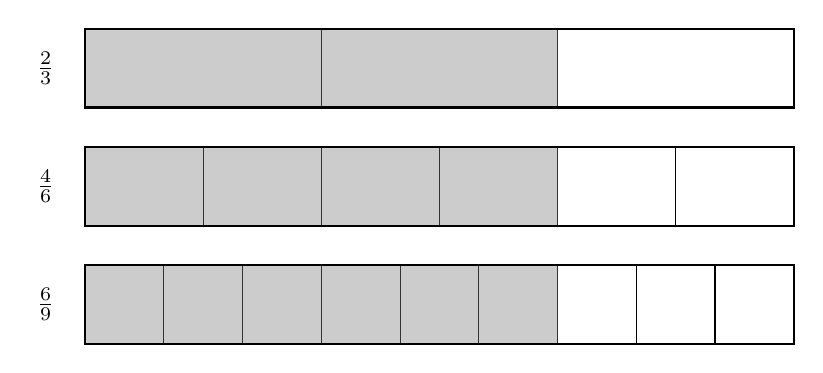
\begin{tikzpicture}
  \draw[step=3cm, black] (0,0) grid (9cm,1cm);
  \fill[gray, opacity=.4] (0,0cm) rectangle (6cm,1cm);
  \draw[black,thick] (0,0) rectangle (9cm,1cm);

  \draw[step=1.5cm, black] (0,-.5cm) grid (9cm,-1.5cm);
  \fill[gray, opacity=.4] (0,-.5cm) rectangle (6cm,-1.5cm);
  \draw[black,thick] (0,-.5cm) rectangle (9cm,-1.5cm);

  \draw[step=1cm, black] (0,-3cm) grid (9cm,-2cm);
  \fill[gray, opacity=.4] (0,-3cm) rectangle (6cm,-2cm);
  \draw[black,thick] (0,-3cm) rectangle (9cm,-2cm);
  
  \node (a) at (-.5cm,.5cm) {$\frac{2}{3}$};
  \node (b) at (-.5cm,-1cm) {$\frac{4}{6}$};
  \node (c) at (-.5cm,-2.5cm) {$\frac{6}{9}$};
\end{tikzpicture}

\end{center}

\begin{definizione}
Si dicono \emph{equivalenti} due frazioni che rappresentano la stessa parte dell'intero.
\end{definizione}

\begin{proprieta}[Invariantiva delle frazioni]
Se si moltiplica, o si divide, numeratore e denominatore di una stessa frazione per uno stesso numero diverso da zero
si ottiene una frazione equivalente alla frazione data.
\end{proprieta}

Per trovare una frazione equivalente a una frazione assegnata è sufficiente moltiplicare per uno stesso
numero il numeratore e il denominatore della frazione assegnata.

\begin{exrig}
 \begin{esempio}
 Trova due frazioni equivalenti a~$\dfrac{4}{7}$.

Moltiplicando numeratore e denominatore per~2 si ha la frazione equivalente:
\[\frac{4\cdot2}{7\cdot2}=\frac{8}{14}.\]
Moltiplicando numeratore e denominatore per~3 si ha la frazione equivalente:
\[\frac{4\cdot3}{7\cdot3}=\frac{12}{21}.\]
 \end{esempio}
\end{exrig}

\begin{definizione}
Una frazione si dice \emph{ridotta ai minimi termini} se il numeratore e il denominatore sono due interi primi tra loro.
\end{definizione}

Per ridurre ai minimi termini una frazione occorre dividere numeratore e denominatore per il loro Massimo Comune Divisore.
%\begin{exrig}
% \begin{esempio}

Per esempio per ridurre ai minimi termini la frazione~$\dfrac{8}{12}$, scompongo in fattori~8 e~12, ottengo~$8=2^3$ e~$12=3\cdot2^2$.
Calcolo il~$\mcd$ prendendo i fattori comuni con l'esponente più piccolo; in questo caso~$2^2$ cioè~4.
Divido numeratore e denominatore per~4:
\[\frac{8}{12} = \frac{8:4}{12:4} = \frac{2}{3}.\]
% \end{esempio}
%\end{exrig}

Tutte le frazioni che hanno il denominatore (numero di parti uguali in cui va divisa l'unità) uguale al numeratore
(numero delle parti che vanno considerate) rappresentano l'intero:

\[\frac{2}{2}=\frac{3}{3}=\frac{10}{10}=1.\]

\begin{wrapfloat}{figure}{r}{0pt}
 % (c) 2012 Dimitrios Vrettos - d.vrettos@gmail.com
% Interi in forma frazionaria
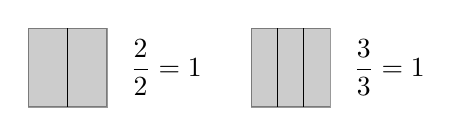
\begin{tikzpicture}

\filldraw[fill=gray, opacity=.4,draw=black] (0,0) rectangle (10mm,10mm);
\draw (5mm,0) -- (5mm,10mm);

\filldraw[fill=gray, opacity=.4,draw=black] (28.333mm,0) rectangle (38.333mm,10mm);
\draw (31.666mm,0) -- (31.666mm,10mm);
\draw (35mm,0) -- (35mm,10mm);

\node (a) at (17.5mm,5mm) {$\displaystyle\frac{2}{2}=1$};
\node (a) at (45.833mm,5mm) {$\displaystyle\frac{3}{3}=1$};

\end{tikzpicture}

\end{wrapfloat}

Per esempio se divido un quadrato in due parti uguali e ne prendo due parti ottengo l'intero;
se divido un quadrato in tre parti uguali e ne prendo tre parti ottengo l'intero \ldots
\vspazio

Cosa significa costruire la grandezza~$\frac{6}{2}$ del quadrato~$Q$?
Tutte le frazioni che hanno il numeratore che è multiplo del denominatore rappresentano un multiplo dell'intero:
\[\frac{6}{2}=3\text{,}\qquad\frac{15}{3}=5\text{,}\qquad\frac{72}{6}=12.\]

\begin{definizione}
 Si chiamano \emph{apparenti} le frazioni che hanno il numeratore multiplo del denominatore;
esse rappresentano una grandezza multipla di quella presa come intero unitario.
\end{definizione}

Le frazioni che hanno il numeratore maggiore del denominatore rappresentano grandezze più grandi dell'intero.
Infatti le parti da considerare (indicate dal numeratore) sono di più delle parti in cui è divisa l'unità
(indicate dal denominatore).
\begin{center}
 % (c) 2012 Dimitrios Vrettos - d.vrettos@gmail.com
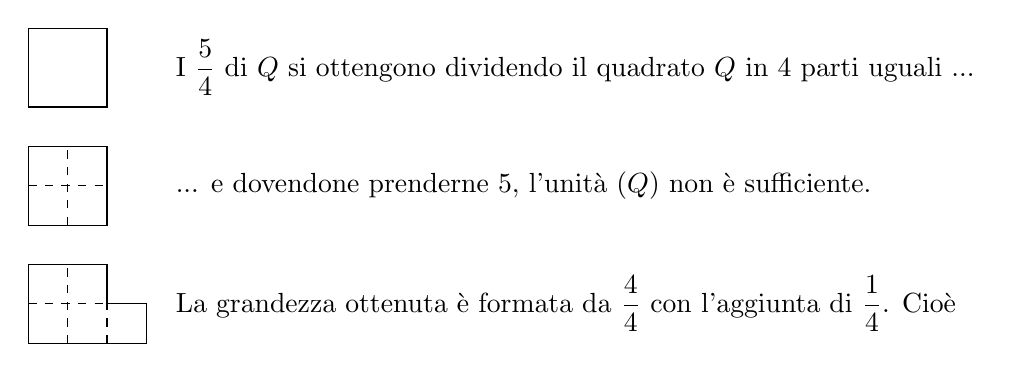
\begin{tikzpicture}

\draw (0,0) rectangle (10mm,10mm);
\draw (0,-15mm) rectangle (10mm,-5mm);
\draw (0,-30mm) -- (0mm,-20mm)--(10mm,-20mm)--(10mm,-25mm)--%
(15mm,-25mm)--(15mm,-30mm)--(0,-30mm);

% \draw[dashed](10mm,-30mm) --(10mm,-25mm);
\begin{scope}[step=5mm, black, dashed]
\draw (0,-15mm) grid (10mm,-5mm);
\draw (0,-30mm) grid (10mm,-20mm);
\end{scope}
\node[right] (a) at (17.5mm,5mm) {I $\displaystyle\frac{5}{4}$ di $Q$ si ottengono dividendo il quadrato $Q$ in 4 parti uguali ...};
\node[right] (b) at (17.5mm,-10mm){... e dovendone prenderne 5, l'unità ($Q$) non è sufficiente.};
\node[right] (b) at (17.5mm,-25mm){La grandezza ottenuta \`e formata da  $\displaystyle\frac{4}{4}$ con l'aggiunta di  $\displaystyle\frac{1}{4}$. Cioè};
\end{tikzpicture}

\end{center}
\[\frac{5}{4}=\frac{4}{4}+\frac{1}{4}=1+\frac{1}{4}.\]

\begin{definizione}
 Si chiamano \emph{improprie} le frazioni che hanno il numeratore maggiore del denominatore;
esse rappresentano una grandezza maggiore della grandezza assegnata come intero.
\end{definizione}

\ovalbox{\risolvii \ref{ese:3.5}, \ref{ese:3.6}, \ref{ese:3.7}, \ref{ese:3.8}, \ref{ese:3.9}, \ref{ese:3.10}, \ref{ese:3.11},
\ref{ese:3.12}, \ref{ese:3.13}, \ref{ese:3.14}, \ref{ese:3.15}, \ref{ese:3.16}, \ref{ese:3.17},}

\vspazio\ovalbox{\ref{ese:3.18}, \ref{ese:3.19}, \ref{ese:3.20}, \ref{ese:3.21}}

\section{Dalle frazioni ai numeri razionali}

Abbiamo visto che ci sono delle frazioni che, pur essendo diverse tra di loro, rappresentano la stessa
parte dell'intero: queste frazioni vengono chiamate \emph{frazioni equivalenti}.
Possiamo formare dei raggruppamenti di frazioni tra loro equivalenti, come nella figura \ref{fig:frazequiv}.

\begin{figure}[ht]
\centering % (c) 2012 Dimitrios Vrettos - d.vrettos@gmail.com
\begin{tikzpicture}
  \begin{scope}[font=\scriptsize]
    %%%%%%%%%%%%%%%%%%%%%%%%
    %  POSIZIONE E DISEGNO %
    %%%%%%%%%%%%%%%%%%%%%%%%    
    \begin{scope}[shape=ellipse,thick, minimum height=30mm, minimum width=40mm]
      \node [name=a, draw=orange] at (0,0) {};
      \node [name=b, draw=blue] at (45mm,0) {};
      \node [name=c, draw=red] at (90mm,0) {};
    \end{scope}
    %%%%%%%%%%%%%%%%%%%%
    %  PARTE SUPERIORE %
    %%%%%%%%%%%%%%%%%%%%
    \begin{scope}[every node/.style={below=1mm}]
      % Primo insieme
      \node  at (a.north west) {$\displaystyle\frac{4}{6}$};
      \node at (a.north) {$\displaystyle\frac{8}{12}$};
      \node  at (a.north east){$\displaystyle\frac{16}{24}$};
      % Secondo insieme
      \node  at (b.north west) {$\displaystyle\frac{7}{6}$};
      \node at (b.north) {$\displaystyle\frac{21}{18}$};
      \node  at (b.north east){$\displaystyle\frac{35}{30}$};
      % Terzo insieme
      \node  at (c.north west) {$\displaystyle\frac{4}{2}$};
      \node at (c.north) {$\displaystyle\frac{8}{4}$};
      \node  at (c.north east){$\displaystyle\frac{30}{15}$};
    \end{scope}
    %%%%%%%%%%%%%%%%%%%
    %  PARTE CENTRALE %
    %%%%%%%%%%%%%%%%%%%
    % Primo e Secondo insieme
    \foreach \x in {a.center,b.center}
      \node at (\x) {\ldots};
    % Terzo insieme
    \node[right=5mm] at (c.center) {\ldots};
    \node[left=5mm] at (c.center) {$2$};
    %%%%%%%%%%%%%%%%%%%%
    %  PARTE INFERIORE %
    %%%%%%%%%%%%%%%%%%%%
    \begin{scope}[every node/.style={above=1mm}]
      % Primo insieme
      \node[above right] at(a.south)  {$\displaystyle\frac{18}{27}$ };
      \node[above left] at(a.south)  {$\displaystyle\frac{6}{9}$};
      \node at(a.south west) {$\displaystyle\frac{2}{3}$};
      \node at(a.south east) {$\displaystyle\frac{10}{15}$};
      % Secondo insieme
      \node at(b.south)  {$\displaystyle\frac{28}{24}$};
      \node at(b.south west) {$\displaystyle\frac{14}{12}$};
      \node at(b.south east) {$\displaystyle\frac{70}{60}$};
      % Terzo insieme
      \node at(c.south)  {$\displaystyle\frac{20}{10}$};
      \node at(c.south west) {$\displaystyle\frac{6}{3}$};
      \node at(c.south east) {$\displaystyle\frac{60}{30}$};
    \end{scope}
  \end{scope}
  %%%%%%%%%%%%%%%%%%%%
  %  TITOLI          %
  %%%%%%%%%%%%%%%%%%%%
  \begin{scope}[font=\small, every node/.style={above=8mm}]
    \node (af) at (a.30) {$\displaystyle\frac{2}{3}$};
    \node (bf) at (b.30) {$\displaystyle\frac{7}{6}$};
    \node (cf) at (c.30) {2};
  \end{scope}
  %%%%%%%%%%%%%%%%%%%%
  % COLLEGAMENTI     %
  %%%%%%%%%%%%%%%%%%%%
  \begin{scope}[thick, ->]
    \draw[orange] (a.north) .. controls +(up:5mm) and +(left:5mm) .. (af) ;
    \draw[blue] (b.north) .. controls +(up:5mm) and +(left:5mm) .. (bf) ;
    \draw[red] (c.north) .. controls +(up:5mm) and +(left:5mm) .. (cf) ;
  \end{scope}
\end{tikzpicture}

\caption{Esempi di frazioni equivalenti.}\label{fig:frazequiv}
\end{figure}

\begin{definizione}
Ogni raggruppamento di frazioni equivalenti è definito come un \emph{numero razionale assoluto}
ed è rappresentato da una qualunque
frazione del raggruppamento; solitamente si sceglie la frazione ridotta ai minimi termini.
\end{definizione}

Nel nostro esempio~$\dfrac{2}{3}$ è il numero razionale rappresentante del raggruppamento
\[\frac{2}{3}=\bigg\lbrace\frac{2}{3}\text{,~}\frac{4}{6}\text{,~}\frac{6}{9}\text{,~}\frac{10}{15}\text{,~}\frac{14}{21}\text{,~}\ldots\bigg\rbrace.\]
In questo modo abbiamo dato al simbolo~$\dfrac{a}{b}$ un nuovo significato, quello di numero e come tale la
scrittura~$\dfrac{a}{b}$ rappresenta il quoziente indicato tra i due numeri naturali~$a$ e~$b$. Scriveremo quindi:~~
$ \dfrac{2}{3} = 2/3 = 2:3 $.

\begin{definizione}
Un numero razionale assoluto preceduto dal segno è detto \emph{numero razionale}.
L'insieme dei numeri razionali si indica con il simbolo~$\insQ$.
\end{definizione}

Il segno del numero razionale relativo è quello che si ottiene dalla regola della
divisione dei segni tra numeratore e denominatore.

\begin{exrig}
\begin{esempio}
Segno di numeri razionali.
\[\frac{-2}{-3}=+\frac{2}{3};\qquad\frac{2}{-3}=-\frac{2}{3};\qquad\frac{-2}{3}=-\frac{2}{3}.\]
\end{esempio}
\end{exrig}

Le frazioni proprie, che hanno numeratore minore del denominatore, rappresentano sempre un numero compreso tra~0 e~1.

\pagebreak

Le frazioni improprie, che hanno numeratore maggiore del denominatore, si possono scrivere come somma di un numero
naturale e di una frazione propria:
\begin{itemize*}
 \item il numero naturale è il risultato della divisione intera tra numeratore e denominatore;
 \item il numeratore della frazione propria è il resto della divisione tra numeratore e denominatore;
 \item il denominatore della frazione propria è il denominatore stesso della frazione.
\end{itemize*}

Le frazioni apparenti, del tipo
$\dfrac{2}{2}$, $\dfrac{6}{3}$, $\dfrac{20}{5}$, $\dfrac{12}{4}$, $\dfrac{12}{3}$, \ldots{}
corrispondono a un numero intero, rispettivamente a~1, 2, 4, 3, 4, \ldots{}

\begin{exrig}
 \begin{esempio}
 ~$\dfrac{11}{3}=3+\dfrac{2}{3}$.
  \begin{itemize*}
   \item $11\divint 3 =3$ il numero naturale;
   \item $11\bmod~3 =2$ il numeratore della frazione propria;
   \item $3$ il denominatore della frazione propria.
  \end{itemize*}
%\[\frac{11}{3}=3+\frac{2}{3}.\]
 \end{esempio}

 \begin{esempio}
 ~$\dfrac{19}{7}=2+\dfrac{5}{7}$.
  \begin{itemize*}
   \item $19\divint 7=2$ il numero naturale;
   \item $19\bmod~7 =~5$ il numeratore della frazione propria;
   \item $7$ il denominatore della frazione propria.
  \end{itemize*}
%\[\frac{19}{7}=2+\frac{5}{7}.\]
 \end{esempio}
\end{exrig}

\ovalbox{\risolvi \ref{ese:3.22}}

\section{La scrittura dei numeri razionali}

I numeri razionali, rappresentati finora come frazioni, possono essere scritti come numeri decimali:
basta fare la divisione tra numeratore e denominatore, il quoziente ottenuto è la
rappresentazione della frazione sotto forma decimale.

\begin{center}
 % (c) 2012 Dimitrios Vrettos - d.vrettos@gmail.com
\begin{tikzpicture}
  \begin{scope}[font=\ttfamily\small,  ]
    \matrix (a) [matrix of nodes]{
    1 &{}&{}&{}&{}&3&{}&{}&{}&{}&{}&{}&[20mm]&1&1&{}&{}&{}&8\\
    1 &0 &{}&{}&{}&|[blue]|0&|[blue]|,&|[blue]|3&|[blue]|3&|[blue]|3&|[blue]|3&|[font=\scriptsize,blue]|\ldots&{}&{}&3&{}&{}&{}&|[blue]|1&|[blue]|,&|[blue]|3&|[blue]|7&|[blue]|5\\
    {}&1 &0 &{}&{}&{}&{}&{}&{}&{}&{}&{}&{}&{}&3&0\\
    &&1&0&&&{}&{}&{}&{}&{}&{}&{}&{}&{}&6&0\\
    &&&1&0&&{}&{}&{}&{}&{}&{}&{}&{}&{}&{}&4&0\\
    &&&&|[font=\scriptsize, red]|\ldots&{}&&{}&{}&{}&{}&{}&{}&{}&{}&{}&{}&|[red]|0\\
    };
  \end{scope}
  \begin{scope}[densely dotted,->]
    \draw (a-1-2.center) -- (a-2-2);
    \draw (a-1-3.center) -- (a-3-3);
    \draw (a-1-4.center) -- (a-4-4);
    \draw (a-1-5.center) -- (a-5-5);

    \draw (a-1-16.center) -- (a-3-16);
    \draw (a-1-17.center) -- (a-4-17);
    \draw (a-1-18.center) -- (a-5-18);
  \end{scope}

  \draw (a-1-6.north west) -- (a-1-6.south west);
  \draw (a-2-6.north west) -- (a-2-11.north east);

  \draw (a-1-19.north west) -- (a-1-19.south west);
  \draw (a-2-19.north west) -- (a-2-23.north east);

  \begin{scope}[font=\small]
    \node[below] at(a-6-6.south) {$\displaystyle\frac{1}{3}=\np{0,3333}\ldots$};
    \node[below=3mm] at(a-6-18.east) {$\displaystyle\frac{11}{8}=\np{1,375}$};
  \end{scope}
\end{tikzpicture}

\end{center}

I numeri decimali che si ottengono sono di due tipi: numeri decimali \emph{finiti} come~$\np{1,375}$ e
numeri decimali \emph{periodici} come~$\np{0,3333}$\ldots;
quest'ultimo si scrive mettendo una barra sulla parte periodica:~$\np{0,}\overline3$ oppure racchiudendo la parte periodica
tra parentesi tonde~$\np{0,}(3)$.

I numeri decimali finiti si ottengono dalle frazioni il cui denominatore ha come fattori solo il~2,
solo il~5 o entrambi, eventualmente elevati a una potenza.

I numeri decimali periodici \emph{semplici} si ottengono dalle frazioni il cui denominatore non ha per fattori né~2 né~5.

I numeri decimali periodici \emph{misti} si ottengono dalle frazioni il cui denominatore contiene altri fattori oltre al~2
e al~5.

\begin{exrig}
 \begin{esempio}
 Alcuni numeri decimali finiti.
\begin{enumeratea}
 \item $\dfrac{11}{8}=\dfrac{11}{2^3}=
\dfrac{11\cdot 5^3}{2^3\cdot 5^3}=\dfrac{\np{1375}}{\np{1000}}=\np{1,375}$;
 \item $\dfrac{7}{25}=\dfrac{7}{5^2}=
\dfrac{7\cdot 2^2}{5^2\cdot 2^2}=\dfrac{28}{100}=\np{0,28}~$;
 \item $\dfrac{13}{40}=\dfrac{13}{2^3\cdot 5}=
\dfrac{13\cdot 5^2}{2^3\cdot 5^3}=\dfrac{325}{\np{1000}}=\np{0,325}$;
 \item $\dfrac{50}{7} = \dfrac{\ldots}{10}$~~non è possibile: non è un decimale finito.
\end{enumeratea}
 \end{esempio}
\end{exrig}

\ovalbox{\risolvi \ref{ese:3.23}}

\begin{procedura}
Trasformare una frazione in numero decimale:
\begin{enumeratea}
 \item eseguire la divisione tra numeratore e denominatore;
 \item se la divisione ha un resto mettere la virgola al quoziente e moltiplicare per~$10$ il resto;
 \item continuare la divisione finché il resto è~$0$ oppure è uguale ad un valore già trovato prima;
 \item se la divisione si conclude con resto~$0$ si ha un numero decimale finito;
 \item se la divisione si conclude perché si è ritrovato un resto ottenuto in precedenza si ha un
numero decimale periodico.
\end{enumeratea}
\end{procedura}

\begin{exrig}
 \begin{esempio}
 Trasformazione di frazioni in numeri decimali.
  \begin{center}
  % (c) 2012 Dimitrios Vrettos - d.vrettos@gmail.com
% Da frazione al decimale
\usetikzlibrary{matrix}

\begin{tikzpicture}
  \begin{scope}[every node/.style={anchor=base,row sep=0pt, column sep =-4.5pt, text depth=0pt, text height=6pt}, matrix anchor=north west, font=\footnotesize]%[font=\ttfamily\scriptsize,matrix anchor=north west]

    \matrix at (0,0) [name= a, matrix of nodes]{
    {}&1&1&3&{}&{}&[2pt]&2&0& &{}\\
    |[gray]|-&1&0&0&{}&{}&&|[blue]|5&|[blue]|,&|[blue]|6&|[blue]|5\\
    {}&{}&1&3&0\\
    {}&|[gray]|-&1&2&0&{}\\
    {}&{}&{}&1&0&0\\
    {}&{}&|[gray]|-&1&0&0&{}\\
    {}&{}&{}&{}&{}&|[red]|0\\};

    \matrix at(39mm,0) [name=b, matrix of nodes]{
    &{}&1&7&{}&{}&[2pt]&6&&&{}\\
    &|[gray]|-&1&2&{}&{}&&|[blue]|2&|[blue]|,&|[blue]|8&|[blue]|3\\
    &{}&{}&5&0\\
    &{}&|[gray]|-&4&8&{}\\
    &{}&{}&{}&2&0\\
    &{}&{}&|[gray]|-&1&8&{}\\
    &{}&{}&{}&{}&|[red]|2\\
    };

    \matrix at (76mm,0) [name=c, matrix of nodes] {
    &{}&1&5&{}&{}&{}&{}&{}&{}&[2pt]&7&&&&&&&{}\\
    &|[gray]|-&1&4&{}&{}&{}&{}&{}&{}&&|[blue]|2&|[blue]|,&|[blue]|1&|[blue]|4&|[blue]|2&|[blue]|8&|[blue]|5&|[blue]|7\\
    &{}&{}&1&0\\
    &{}&|[gray]|-&{}&7&{}\\
    &{}&{}&{}&3&0\\
    &{}&{}&|[gray]|-&2&8&{}\\
    &{}&{}&{}&{}&2&0\\
    &{}&{}&{}&|[gray]|-&1&4&{}\\
    &{}&{}&{}&{}&{}&6&0\\
    &{}&{}&{}&{}&|[gray]|-&5&6&{}\\
    &{}&{}&{}&{}&{}&{}&4&0\\
    &{}&{}&{}&{}&{}&|[gray]|-&3&5&{}\\
    &{}&{}&{}&{}&{}&{}&{}&5&0\\
    &{}&{}&{}&{}&{}&{}&|[gray]|-&4&9&{}\\
    &{}&{}&{}&{}&{}&{}&{}&{}&|[red]|1\\
    };

  \end{scope}
  % Prima divisione
  \draw (a-1-8.north west) -- (a-2-8.south west);
  \draw (a-1-8.south west) -- (a-1-11.south east);
  \draw[gray] (a-2-1.south east) -- (a-2-5.south west);
  \draw[gray] (a-4-2.south east) -- (a-4-6.south west);
  \draw[gray] (a-6-3.south east) -- (a-6-7.south west);

  % Seconda divisione
  \draw (b-1-8.north west) -- (b-2-8.south west);
  \draw (b-1-8.south west) -- (b-1-11.south east);
  \draw[gray] (b-2-2.south east) -- (b-2-5.south west);
  \draw[gray] (b-4-3.south east) -- (b-4-6.south west);
  \draw[gray] (b-6-4.south east) -- (b-6-7.south west);

  % Terza divisione
  \draw (c-1-12.north west) -- (c-2-12.south west);
  \draw (c-1-12.south west) -- (c-1-19.south east);
  \draw[gray] (c-2-2.south east) -- (c-2-5.south west);
  \draw[gray] (c-4-3.south east) -- (c-4-6.south west);
  \draw[gray] (c-6-4.south east) -- (c-6-7.south west);
  \draw[gray] (c-8-5.south east) -- (c-8-8.south west);
  \draw[gray] (c-10-6.south east) -- (c-10-9.south west);
  \draw[gray] (c-12-7.south east) -- (c-12-10.south west);
  \draw[gray] (c-14-8.south east) -- (c-14-11.south west);

  \begin{scope}[gray, dashed, densely dotted, ->]
    \draw (a-1-5.center) -- (a-3-5);
    \draw (a-1-6.center) -- (a-5-6);

    \draw (b-1-5.center) -- (b-3-5);
    \draw (b-1-6.center) -- (b-5-6);

    \draw (c-1-5.center) -- (c-3-5);
    \draw (c-1-6.center) -- (c-5-6);
    \draw (c-1-7.center) -- (c-7-7);
    \draw (c-1-8.center) -- (c-9-8);
    \draw (c-1-9.center) -- (c-11-9);
    \draw (c-1-10.center) -- (c-13-10);
  \end{scope}
  \begin{scope}[font=\small]
    \node[above=5pt]  at (a-1-6.north) {a)};
    \node[above=5pt]  at (b-1-6.north) {b)};
    \node[above=5pt]  at (c-1-10.north) {c)};
  \end{scope}
\end{tikzpicture}
	
  \end{center}	
  \begin{enumeratea}
  \item $\dfrac{113}{20}=\np{5,65}\:$ numero decimale finito;\vspace{1.03ex}
  \item $\dfrac{17}{6}=\np{2,8}\overline{3}\:$ numero decimale periodico misto di periodo~3;\vspace{1.03ex}
  \item $\dfrac{15}{7}=\np{2,}\overline{142\,857}\:$ numero decimale periodico di periodo~$\np{142857}$.
  \end{enumeratea}
 \end{esempio}
\end{exrig}

\ovalbox{\risolvi \ref{ese:3.24}, \ref{ese:3.25}, \ref{ese:3.26}}\vspazio

Viceversa un numero decimale finito o periodico può essere sempre scritto sotto forma di frazione.

\begin{procedura}
	Trasformare un numero decimale finito in una frazione:
\begin{enumeratea}
 \item contare le cifre significative dopo la virgola;
 \item moltiplicare numeratore e denominatore per la potenza del~$10$ che ha esponente uguale al
	 numero delle cifre significative dopo la virgola.
\end{enumeratea}
\end{procedura}

Per facilitare questa operazione possiamo considerare i numeri decimali finiti come frazioni
particolari che hanno il numeratore uguale al numero decimale e il denominatore uguale a~1.

Ad esempio, il numero~$\np{1,360}$ ha due cifre significative dopo la virgola, quindi:
\[\frac{\np{1,36}}{1}=\frac{\np{1,36}\cdot10^2}{1\cdot10^2}=\frac{136}{100}=\frac{34}{25}\]
ed il numero~$\np{0,00043000}$ ha cinque cifre significative dopo la virgola, quindi:
\[\frac{\np{0,00043}}{1}=\frac{\np{0,00043}\cdot10^5}{1\cdot10^5}=\frac{43}{\np{100000}}.\]

Un numero decimale periodico, generalmente, presenta tre elementi:
\begin{description}
 \item [la parte intera] composta dalle cifre poste prima della virgola;
 \item [il periodo] che è composto da una o più cifre che si ripetono all'infinito dopo la virgola;
 \item [l'antiperiodo] la parte, talvolta assente, composta da una o più cifre poste tra la virgola e il periodo.
\end{description}


Per esempio, nel numero~$\np{253,485795795795795}\ldots$ la parte intera è~$253$, il periodo è~$579$ e l'antiperiodo è~$48$.
Dato che il numero è infinito non può essere scritto con tutte le sue cifre, si usano due modi per scriverlo in
forma compatta, mettendo una lineetta sopra le cifre del periodo o racchiudendo le cifre del periodo tra
parentesi tonde. Quindi può essere rappresentato come~$\np{253,48}\overline{5\,79}$, oppure~$\np{253,48}(5\,79)$.

I numeri decimali periodici si dividono in:
\begin{description}
 \item [semplici] se subito dopo la virgola è presente il periodo (non hanno antiperiodo);
 \item [misti] se dopo la virgola è presente l'antiperiodo.
\end{description}

Anche i numeri periodici possono essere trasformati in una frazione, che si
dice \emph{frazione generatrice} del numero.

\begin{procedura}
 Determinare la frazione generatrice di un numero periodico:
\begin{enumeratea}
\item scrivere il numero senza la virgola;
\item il numeratore della frazione si ottiene sottraendo dal numero senza la virgola il numero
	 costituito dalle cifre che precedono il periodo;
\item il denominatore della frazione si ottiene scrivendo tanti~$9$ quante sono le cifre del periodo e
	 tanti~$0$ quante sono le eventuali cifre dell'antiperiodo.
\end{enumeratea}
\end{procedura}

\begin{exrig}
 \begin{esempio}
 Trasformare il numero periodico $\np{2,5}\overline{12}$ nella frazione equivalente.
  \begin{enumeratea}
  \item $\np{2,5}\overline{12}\rightarrow~\np{2512}\:$ scrivo il numero senza la virgola; %\vspace{1.03ex}
  \item $\np{2512}-25=\np{2487}\:$ determino il numeratore della frazione; %\vspace{1.03ex}
  \item $990\:$ determino il denominatore della frazione. In definitiva:
  \[\np{2,5}\overline{12}=\frac{2512-25}{990}=\dfrac{\np{2487}}{990}\]
  \end{enumeratea}
 \end{esempio}
\end{exrig}

%\paragraph*{Passo~$a$}~$\np{2,5}\overline{12}\rightarrow~\np{2512}$.
%\paragraph*{Passo~$b$}~$\np{2512}-25=\np{2487}$.
%\paragraph*{Passo~$c$}~$\np{2,5}\overline{12}=\dfrac{\np{2487}}{990}$.


\paragraph*{Ma perché questa regola? Una possibile spiegazione}
Consideriamo il numero periodico semplice~$\np{2,}\overline{3}$.
Poiché $\np{2,}\overline{3} \cdot 10 = \np{23,}\overline{3}$ si ha che $\np{2,}\overline{3} \cdot 9 = \np{23,}\overline{3} - \np{2,}\overline{3} = 21$.
Quindi, consideriamo la frazione~$\frac{\np{2,}\overline{3}}{1}$ e moltiplichiamo numeratore e denominatore per~$9$, così da far sparire
la parte periodica al numeratore. Si ha quindi
\[\np{2,}\overline{3}=\frac{\np{2,}\overline{3}\cdot 9}{9}=\frac{21}{9}=\frac{7}{3}.\]

% Considero la frazione~$\frac{2,\overline{3}}{1}$
%moltiplico numeratore e denominatore per~$10$ e quindi ottengo~$\frac{2,\overline{3}\cdot10}{1\cdot10} = \frac{23,\overline{3}}{10}$.
%
%L'obiettivo è quello di eliminare dal numeratore della frazione la parte decimale.
%Per ottenere questo risultato tolgo~$2,\overline{3}$ da~$23,\overline{3}$, cioè
%$23,\overline{3}-2,\overline{3}=21$.
%
%Come mai~$2,\overline{3}$ e non~$1,\overline{3}$ o~$0,\overline{3}$?
%Perché in questo modo posso sapere quanto vale il denominatore: se~$23,\overline{3}$ è il risultato
%della moltiplicazione di~$2,\overline{3}\cdot10$,~$21$~è il risultato della moltiplicazione di
%$2,\overline{3}\cdot9$ in quanto~$23,\overline{3}-2,\overline{3}=21$. Quindi anche il denominatore
%deve essere moltiplicato per~$9$ e non per~$10$.
%In definitiva
%\[2,\overline{3}=\frac{2,\overline{3}\cdot 9}{9}=\frac{21}{9}=\frac{7}{3}.\]

Possiamo usare lo stesso procedimento per il numero periodico misto~$\np{2,5}\overline{12}$.
Poiché $\np{2,5}\overline{12} \cdot \np{1000} = \np{2512,}\overline{12}$ si ha che $\np{2,5}\overline{12} \cdot 990 = \np{2512,}\overline{12} - \np{25,}\overline{12} = \np{2487}$.
Quindi, consideriamo la frazione~$\frac{\np{2,5}\overline{12}}{1}$ e moltiplichiamo numeratore e denominatore per~$990$, così da far sparire
la parte periodica al numeratore. Si ha quindi
\[\np{2,5}\overline{12}=\frac{\np{2,5}\overline{12} \cdot 990}{990}=\frac{\np{2487}}{990}.\]

%Considero la frazione~$\frac{2,5\overline{12}}{1}$, moltiplico numeratore e denominatore per~$1\,000$ e ottengo:
%$\frac{2512,\overline{12}}{1\,000}$.
%L'obiettivo è quello di eliminare dal numeratore della frazione la parte decimale che contiene il periodo che
%si ripete all'infinito. Per ottenere questo risultato tolgo da~$2\,512,\overline{12}$ il valore~$25,\overline{12}$, cioè~$2\,512,\overline{12}-25,\overline{12}=2\,487$.
%Per avere una frazione equivalente occorre che al denominatore abbia~$990$ in quanto dal numeratore ho tolto~$10$ volte
%$2,5\overline{12}$.
%\[2,5\overline{12}=\frac{2\,512-25}{990}=\frac{2\,487}{990}.\]

\subsection{Numeri periodici particolari}

Numeri periodici particolari sono quelli che hanno come periodo il numero~$9$,
come~$\np{2,}\overline{9}$, $\np{1,1}\overline{9}$, $\np{21,22}\overline{9}$, ecc.
Se, per esempio, applichiamo la regola per il calcolo della frazione generatrice al numero periodico
otteniamo un risultato inatteso
\[\np{2,}\overline{9}=\frac{29-2}{9}=\frac{27}{9}=3.\]
Quindi~$\np{2,}\overline{9}$ coincide con il numero intero~$3$.
Per lo stesso motivo~$\np{1,1}\overline{9}=\np{1,2}$ e~$\np{21,22}\overline{9}=\np{21,23}$.
\pagebreak
\begin{wrapfloat}{figure}{r}{0pt}
% (c) 2012 Dimitrios Vrettos - d.vrettos@gmail.com
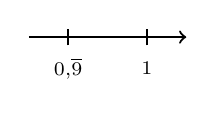
\begin{tikzpicture}
  \begin{scope}[thick,font=\scriptsize]
  \draw[->] (0,0) -- (20mm,0);
  \foreach \n in {5mm,15mm}{%
    \draw (\n,-3pt) -- (\n,3pt);}
  \node (p) at (5mm,-4mm) {$0,\!\overline{9}$};
  \node (i) at (15mm,-4mm) {$1$};
  \end{scope}
\end{tikzpicture}

\end{wrapfloat}

Questo fatto si può anche dimostrare in modo grafico, rappresentando, ad esempio, il numero~$\np{0,}\overline{9}$ e
il numero~$1$ sulla retta reale.\footnote{si veda la sezione~\ref{sect:intro_numeri_reali} a pagina~\pageref{sect:intro_numeri_reali}.}
Se i due numeri fossero diversi sarebbero rappresentati da due punti distinti
come in figura. Dato che la retta reale non può avere ``buchi'',
tra due punti distinti ce ne deve essere almeno un altro corrispondente ad un numero compreso tra i primi due.
Ma qual è questo numero? Qualunque numero decimale minore di~$1$ è sicuramente superato dal numero~$\np{0,}\overline{9}$,
ad esempio~$\np{0,9999999998}$ è sicuramente più piccolo di~$\np{0,}\overline{9}$. Quindi non può esistere nessun numero tra
$\np{0,}\overline{9}$ e~$1$,
di conseguenza i due numeri coincidono.

\ovalbox{\risolvii \ref{ese:3.27}, \ref{ese:3.28}, \ref{ese:3.29}, \ref{ese:3.30}, \ref{ese:3.31}, \ref{ese:3.32}}

\section{I numeri razionali e la retta}

Anche i numeri razionali si possono rappresentare su una retta orientata. Per fare questo occorre
scegliere un punto~$O$ sulla retta e associare ad esso il numero~0. Fissiamo poi un segmento unitario e scegliamo
un verso di percorrenza.

Un numero razionale positivo, rappresentato dalla frazione~$\frac{a}{n}$, corrisponde a un punto della retta determinato nel seguente modo.

Dividiamo il segmento unitario~$u$ in tante parti uguali
quante sono quelle indicate dal denominatore~$n$ della frazione, ottenendo così la frazione unitaria~$\frac{1}{n}$.
A partire dal punto di origine~$O$, procedendo verso destra, si contano~$a$ frazioni unitarie.
L'ultimo punto rappresenta il numero razionale~$\frac{a}{n}$.

Per le frazioni improprie la singola unità~$u$ non è sufficiente, occorre prendere quella successiva e
dividere anche questa in~$n$ parti. Il procedimento si ripete fino a che si considerano tutte
le frazioni unitarie indicate da~$a$. Anche in questo caso, il punto individuato dall'ultima frazione unitaria
rappresenta il numero razionale~$\frac{a}{n}$.

In alternativa si può scomporre la frazione impropria
nella somma di un numero intero e di una frazione propria, quindi si rappresenta la frazione impropria
a partire dal suo numero intero invece che partire da~0.
Per esempio, per rappresentare la frazione~$\frac{3}{2}$
trasformiamo la frazione in~$1+\frac{1}{2}$, quindi per indicare~$\frac{3}{2}$ possiamo rappresentare~$\frac{1}{2}$ partendo da~1.

Se il numero razionale è negativo, ci muoviamo nel senso opposto, cioè da destra verso sinistra.

\begin{center}
% (c) 2012 Dimitrios Vrettos - d.vrettos@gmail.com
% (c) 2014 Daniele Masini - d.masini.it@gmail.com
\begin{tikzpicture}[font=\small]
\begin{scope}[thin,gray,xscale=2.5]
\foreach \x/\xtext in {%
-1,-.875,...,2
}
\draw[shift={(\x,0)}] (0pt,2pt) -- (0pt,-2pt);
\end{scope}
\begin{scope}[thick,xscale=2.5]
\draw[->] (-1.2,0) -- (2.2,0) node [above] () {$\insQ$};
\foreach \x/\xtext in {%
-1,0,1,2}
\draw[shift={(\x,0)}] (0pt,2pt) -- (0pt,-2pt) node[below] {$\xtext$};
\draw (0,0.5) -- node[above] {$u$} (1,0.5);
\draw (0,0.4) -- (0,0.6);
\draw (1,0.4) -- (1,0.6);
\end{scope}
\begin{scope}[scale=2.5]
\draw[fill] (1.5,0) circle (.5pt) node[below] {$\dfrac{3}{2}$};
\draw[fill] (-0.75,0) circle (.5pt) node[below] {$-\dfrac{3}{4}$};
\draw[fill] (0.625,0) circle (.5pt) node[below] {$\dfrac{5}{8}$};
\end{scope}

\end{tikzpicture}

\end{center}

\ovalbox{\risolvii \ref{ese:3.33}, \ref{ese:3.34}, \ref{ese:3.35}}

\section{Confronto tra numeri razionali}

Il numero razionale rappresentato dalla frazione~$\frac{a}{n}$ è \emph{minore} del numero razionale
rappresentato dalla frazione~$\frac{b}{m}$, se nella retta orientata il punto che corrisponde alla
frazione~$\frac{a}{n}$ precede il punto che corrisponde alla frazione~$\frac{b}{m}$ e si scrive\ \  $\frac{a}{n}<\frac{b}{m}$.

Viceversa il numero razionale~$\frac{a}{n}$ è \emph{maggiore} di~$\frac{b}{m}$
se nella retta orientata il punto che corrisponde alla frazione~$\frac{a}{n}$ segue il punto che corrisponde alla frazione~$\frac{b}{m}$ e si scrive\ \ $\frac{a}{n}>\frac{b}{m}$.

Infine il numero razionale~$\frac{a}{n}$ è \emph{equivalente} a~$\frac{b}{m}$ se nella retta orientata i punti che corrispondono alle frazioni~$\frac{a}{n}$ e~$\frac{b}{m}$ coincidono e si scrive\ \ $\frac{a}{n} = \frac{b}{m}$.

\begin{exrig}
\begin{esempio}
Confronto tra numeri razionali.
\begin{center}
% (c) 2014 Daniele Masini - d.masini.it@gmail.com
\begin{tikzpicture}
\begin{scope}[thick,font=\small]
\draw[->] (-10pt,0) -- (240pt,0) node [above] () {$\insQ$};
\foreach \x/\xtext in {%
0/-2,.75/-\dfrac{13}{8},2/-1,3/-\dfrac{1}{2},%
4/0,4.75/\dfrac {3}{8},%
6/1,7/\dfrac{3}{2},8/2}
\draw[shift={(\x,0)}] (0pt,2pt) -- (0pt,-2pt) node[below] {$\xtext$};
\draw (.75,0) circle (1pt);
\draw (3,0) circle (1pt);
\draw (4.75,0) circle (1pt);
\draw (7,0) circle (1pt);
\end{scope}
\end{tikzpicture}

\end{center}
\[-\frac{13}{8}<-\frac{1}{2}\text{,}\qquad\frac{3}{8}>-\frac{1}{2}\text{,}\qquad\frac{3}{8}<\frac{3}{2}\text{,}\qquad-1>-\frac{13}{8}.\]
\end{esempio}
\end{exrig}

Per alcune frazioni è facile vedere se una frazione è minore o maggiore di un'altra. Ma non sempre è così semplice.

Consideriamo per esempio le frazioni~$\frac{7}{9}$ e~$\frac{6}{7}$.
Quale frazione precede e quale segue? Il confronto non è immediato perché con la prima frazione si conta per
unità frazionarie di tipo~$\frac{1}{9}$ e con la seconda per unità frazionarie di tipo~$\frac{1}{7}$.

In generale, senza ricorrere alla rappresentazione sulla retta, come si possono confrontare i numeri razionali?

Conviene sostituire le frazioni date con altre equivalenti che hanno le stesse unità frazionarie:
cioè occorre ridurre le frazioni allo stesso denominatore.

\begin{procedura}
	Confrontare due frazioni:
\begin{enumeratea}
\item si calcola il minimo comune multiplo ($\mcm$) dei denominatori delle frazioni;
\item si trasforma ciascuna frazione come segue:
\subitem il nuovo denominatore è il~$\mcm$ trovato;
\subitem il nuovo numeratore si ottiene dividendo il~$\mcm$ per il denominatore della
	  frazione data e moltiplicando il quoziente ottenuto per il numeratore della frazione data.
\item si confrontano i nuovi numeratori: la frazione più grande è quella che ha il numeratore più
	grande.
\end{enumeratea}
\end{procedura}
%\pagebreak
\begin{exrig}
\begin{esempio}
Confronta le frazioni~$\dfrac{7}{9}$ e~$\dfrac{6}{7}$.

$\mcm(7\text{,~}9)=63$.
\[\frac{7}{9}=\frac{7\cdot7}{9\cdot7}=\frac{49}{63}\text{,}\qquad%
\frac{6}{7}=\frac{6\cdot9}{7\cdot9}=\frac{54}{63}.\]
\[\frac{54}{63}>\frac{49}{63}\quad\Rightarrow\quad\frac{6}{7}>\frac{7}{9}.\]
\end{esempio}
\end{exrig}

Un altro modo per confrontare due frazioni consiste nel \emph{moltiplicare in croce} numeratori e
denominatori delle frazioni, come nei seguenti esempi.

\pagebreak
\begin{exrig}
\begin{esempio}
Confronta~$\dfrac{3}{2}$ con~$\dfrac{5}{3}$.

Moltiplichiamo il numeratore della prima frazione per il denominatore della seconda frazione e
il denominatore della prima per il denominatore della seconda

 \[3\cdot3=9 \qquad 2\cdot5=10.\]

Quindi, poiché $9<10$ si può scrivere

 \[\dfrac{3}{2}<\dfrac{5}{3}.\]

\end{esempio}
\end{exrig}

\ovalbox{\risolvii \ref{ese:3.36}, \ref{ese:3.37}, \ref{ese:3.38}, \ref{ese:3.39}, \ref{ese:3.40}, \ref{ese:3.41}, \ref{ese:3.42}, \ref{ese:3.43}, \ref{ese:3.44}}

\section{Le operazioni con i numeri razionali}
Con i numeri razionali è sempre possibile eseguire le addizioni, le moltiplicazioni, le sottrazioni e le divisioni.
In altre parole, poiché un numero razionale può essere scritto sotto forma di frazione, se si addizionano,
si moltiplicano, si sottraggono, si dividono due frazioni il risultato è sempre una frazione.

\subsection{Addizione}

Se due frazioni hanno la stessa unità frazionaria allora è sufficiente sommare i numeratori delle frazioni
e prendere come denominatore l'unità frazionaria comune.
\[\frac{5}{3}+\frac{2}{3}=\frac{5+2}{3}=\frac{7}{3}.\]
%
%\begin{center}
%% (c) 2012 Dimitrios Vrettos - d.vrettos@gmail.com
\begin{tikzpicture}
  \draw (0,0) rectangle  (10mm,10mm);
  \begin{scope}[font=\Huge]
    \node at  (5mm,5mm) {$+$};
  \end{scope}
  \begin{scope}[font=\small]
    \node (a) at (-15mm,10mm) {$\displaystyle\frac{5}{3}$};
    \node (b) at (-15mm,0mm) {$\displaystyle\frac{2}{3}$};
    \node (c) at (25mm,5mm) {$\displaystyle\frac{7}{3}$};
  \end{scope}
  \node (entrata) at (0,5mm) {};
  \node (uscita) at (10mm,5mm) {};
  \begin{scope}[->,concept connection,blue,thin]
    \draw (a) -- (entrata);
    \draw (b) -- (entrata);
    \draw (uscita) -- (c);
  \end{scope}
\end{tikzpicture}

%\end{center}

\begin{definizione}
La \emph{somma di due frazioni con lo stesso denominatore} è una frazione che ha per denominatore lo stesso
denominatore delle frazioni date e per numeratore la somma dei numeratori.
\end{definizione}


Se le unità frazionarie sono diverse dobbiamo considerare frazioni equivalenti a quelle date che abbiano la
stessa unità frazionaria e poi eseguire l'addizione come indicato nel punto precedente e cioè
sommando i numeratori e lasciando lo stesso denominatore comune.

\begin{center}
% (c) 2012 Dimitrios Vrettos - d.vrettos@gmail.com
\begin{tikzpicture}
  \draw (0,0) rectangle  (10mm,10mm);
  \begin{scope}[font=\Huge]
    \node at  (5mm,5mm) {$+$};
  \end{scope}
  \begin{scope}[font=\small]
    \node [left](a) at (-12.5mm,10mm) {$\displaystyle{\frac{5}{3}=\frac{25}{15}}$};
    \node [left](b) at (-12.5mm,0mm) {$\displaystyle{\frac{2}{3}=\frac{6}{15}}$};
    \node (c) at (25mm,5mm) {$\displaystyle\frac{31}{15}$};
  \end{scope}
  \node (entrata) at (0,5mm) {};
  \node (uscita) at (10mm,5mm) {};
  \begin{scope}[->,concept connection,blue,thin]
    \draw (a) -- (entrata);
    \draw (b) -- (entrata);
    \draw (uscita) -- (c);
  \end{scope}
\end{tikzpicture}

\end{center}

In generale, la somma di due frazioni~$\dfrac{m}{n}+\dfrac{p}{q}$ si può scrivere come $\dfrac{m\cdot q +n\cdot p}{n\cdot q}$.

\begin{center}
% (c) 2012 Dimitrios Vrettos - d.vrettos@gmail.com
\begin{tikzpicture}
  \draw (0,0) rectangle  (10mm,10mm);
  \begin{scope}[font=\Huge]
    \node at  (5mm,5mm) {$+$};
  \end{scope}
  \begin{scope}[font=\small]
    \node [left](a) at (-12.5mm,10mm) {$\displaystyle{\frac{m}{n}=\frac{m\cdot q}{n\cdot q}}$};
    \node [left](b) at (-12.5mm,0mm) {$\displaystyle{\frac{p}{q}=\frac{n\cdot p}{n\cdot q}}$};
    \node [right](c) at (25mm,5mm) {$\displaystyle\frac{m\cdot q+n\cdot p}{n\cdot q}$};
  \end{scope}
  \node (entrata) at (0,5mm) {};
  \node (uscita) at (10mm,5mm) {};
  \begin{scope}[->,concept connection,blue,thin]
    \draw (a) -- (entrata);
    \draw (b) -- (entrata);
    \draw (uscita) -- (c);
  \end{scope}
\end{tikzpicture}

\end{center}

Quando si sommano due frazioni si può scegliere un qualsiasi denominatore comune, tuttavia per semplificare i calcoli conviene scegliere il più piccolo possibile, cioè il minimo comune multiplo dei denominatori delle frazioni da sommare.

\begin{procedura}
Sommare due o più frazioni:
\begin{enumeratea}
\item ridurre le frazioni ai minimi termini;
\item calcolare il~$\mcm$ dei denominatori;
\item mettere il~$\mcm$ come denominatore della frazione somma;
\item per ogni frazione dividere il~$\mcm$ per il suo denominatore e moltiplicare il risultato per il
numeratore della frazione mantenendo il segno;
\item calcolare la somma algebrica di tutti i numeri trovati;
\item mettere la somma ottenuta come numeratore della frazione somma;
\item ridurre ai minimi termini la frazione ottenuta.
\end{enumeratea}
\end{procedura}
\begin{exrig}
 \begin{esempio}
Sommare le frazioni~$\dfrac{8}{12}-\dfrac{5}{6}+\dfrac{8}{5}-1$.
 \begin{enumeratea}
  \item riduco ai minimi termini le frazioni
  ${\dfrac{2}{3}-\dfrac{5}{6}+\dfrac{8}{5}-\dfrac{1}{1}}$;
  \item calcolo~$\mcm(3\text{,~}6\text{,~}5\text{,~}1)=30$;
  \item la frazione somma avrà come denominatore il~$\mcm$ trovato~$\dfrac{\ldots}{30}$;
  \item per ogni frazione divido il~$\mcm$ per il suo denominatore e moltiplico il risultato
  per il numeratore:
  \begin{align*}
  \frac{2\cdot(30:3)-5\cdot(30:6)+8\cdot(30:5)-1\cdot(30:1)}{30}&=
  \frac{2\cdot10-5\cdot5+8\cdot6-1\cdot30}{30}\\
  &=\frac{20-25+48-30}{30};
  \end{align*}
  \item calcolo la somma algebrica dei numeri ottenuti al numeratore~$+13$;
  \item metto la somma ottenuta al numeratore della frazione somma~$+\dfrac{13}{30}$;
  \item vedo se posso ridurre la frazione, in questo caso no, il risultato è~$+\dfrac{13}{30}$.
 \end{enumeratea}
 \end{esempio}
%\end{exrig}
\begin{comment}
%\begin{exrig}
\begin{esempio}
Sommare le frazioni~$\dfrac{8}{12}-\dfrac{5}{6}+\dfrac{8}{5}-1$.

\paragraph*{Passo~$a$} riduco ai minimi termini le frazioni
$\displaystyle{\frac{2}{3}-\frac{5}{6}+\frac{8}{5}-\frac{1}{1}}$
\paragraph*{Passo~$b$} calcolo~$\mcm(3\text{,~}6\text{,~}5\text{,~}1)=30$
\paragraph*{Passo~$c$} la frazione somma avrà come denominatore il~$\mcm$ trovato~$\dfrac{\ldots}{30}$
\paragraph*{Passo~$d$} per ogni frazione divido il~$\mcm$ per il suo denominatore e moltiplico il risultato
per il numeratore:
\begin{align*}
\frac{2\cdot(30:3)-5\cdot(30:6)+8\cdot(30:5)-1\cdot(30:1)}{30}&=
\frac{2\cdot10-5\cdot5+8\cdot6-1\cdot30}{30}\\
&=\frac{20-25+48-30}{30}
\end{align*}

\paragraph*{Passo~$e$} calcolo la somma algebrica dei numeri ottenuti al numeratore~$+13$
\paragraph*{Passo~$f$} metto la somma ottenuta al numeratore della frazione somma~$+\dfrac{13}{30}$
\paragraph*{Passo~$g$} vedo se posso ridurre la frazione, in questo caso no, il risultato è~$+\dfrac{13}{30}$.
\end{esempio}
\end{comment}
\begin{esempio}
Sommare i numeri razionali~$-\np{0,2}-\np{1,}\overline{2}+25\%+\dfrac{7}{12}$.

Trasformo i numeri razionali in frazioni: 
\[-\frac{2}{10}-\frac{12-1}{9}+\frac{25}{100}+\frac{7}{12}=-\frac{1}{5}-\frac{11}{9}+\frac{1}{4}+\frac{7}{12}.\]

Quindi~$\mcm(5\text{,~}9\text{,~}4\text{,~}12)=180$.

\begin{align*}
\frac{-1\cdot(180:5)-11\cdot(180:9)+1\cdot(180:4)+7\cdot(180:12)}{180}&=
\frac{-1\cdot36-11\cdot20+1\cdot45+7\cdot15}{180}\\
&=\frac{-36-220+45+105}{180}\\
&=-\frac{106}{180} \\
&=-\frac{53}{90}.
\end{align*}
\end{esempio}
\end{exrig}

\subsection{Sottrazione di frazioni}

La sottrazione di frazioni si può sempre trasformare in una addizione tra la prima frazione e
l'opposto della seconda frazione. Come per i numeri relativi, quando si parla di
somma di frazioni si intende sempre somma algebrica di frazioni.

\vspazio\ovalbox{\risolvii \ref{ese:3.45}, \ref{ese:3.46}, \ref{ese:3.47}, \ref{ese:3.48}, \ref{ese:3.49}, \ref{ese:3.50}}

\subsection{Moltiplicazione}
\begin{multicols}{2}
Il prodotto tra frazioni può essere interpretato come l'area di un rettangolo in cui
le frazioni fattori sono la base e l'altezza.

Moltiplicare~$\frac{4}{5}\cdot\frac{2}{3}$ è come calcolare l'area del rettangolo di base~$\frac{4}{5}$ e altezza
$\frac{2}{3}$. 
Ogni rettangolino di base~$\frac{1}{5}$ e altezza~$\frac{1}{3}$ ha area~$\frac{1}{15}$.
I rettangolini da prendere in considerazione sono~8. Il risultato è quindi~$\frac{8}{15}$. 
Il denominatore indica in quante parti è stato diviso il quadrato unitario: sono $3 \cdot 5=15$ parti.
Il numeratore indica quante parti prendiamo, sono le parti $2\cdot 4=8$ in grigio. 
\begin{center}
 % (c) 2012 Dimitrios Vrettos - d.vrettos@gmail.com
\tikzset{brace/.style={decoration={brace, mirror},decorate}}

\begin{tikzpicture}[font=\small]
  \begin{scope}[x=6mm,y=10mm]
    \foreach \x in {0,1,2,3,4}
      \foreach \y in {0,1,2}
	\draw (\x,\y) rectangle (\x+1,\y+1);
    \foreach \x in {0,1,...,3}
      \foreach \y in {0,1}{
	\fill[gray, opacity=.4](\x,\y) rectangle (\x+1,\y+1);
	\draw (\x+.5,\y+.5) node [rectangle] () {$\dfrac{1}{15}$};
      }

    \draw (4.5,2.5) node [rectangle] () {$\dfrac{1}{15}$};

    \begin{scope}[|-|,above]
      \draw (0,3.2) -- (5,3.2) node [pos=.5] () {$1\text{ unità}$};
      \draw (5.33,0)--(5.33,3)node [rotate=-90,pos=.5] () {$1\text{ unità}$};
    \end{scope}

    \draw[brace] (0,-.1) --  (4,-.1) node [below, pos=0.5] {$\dfrac{4}{5}$};
    \draw[brace] (-.2,2) --  (-.2,0) node [left, pos=0.5] {$\dfrac{2}{3}$};
  \end{scope}
  
\end{tikzpicture}

\end{center}
\end{multicols}

\begin{definizione}
Il \emph{prodotto di due frazioni} è una frazione che ha per numeratore il prodotto dei numeratori
e per denominatore il prodotto dei denominatori.
\end{definizione}

\begin{center}
 % (c) 2012 Dimitrios Vrettos - d.vrettos@gmail.com
\begin{tikzpicture}
  \draw (0,0) rectangle  (10mm,10mm);
  \begin{scope}[font=\Huge]
    \node at  (5mm,5mm) {$\cdot$};
  \end{scope}
  \begin{scope}[font=\small]
    \node (a) at (-15mm,10mm) {$\displaystyle\frac{m}{n}$};
    \node (b) at (-15mm,0mm) {$\displaystyle\frac{p}{q}$};
    \node (c) at (25mm,5mm) {$\displaystyle\frac{m\cdot p}{n\cdot q}$};
  \end{scope}
  \node (entrata) at (0,5mm) {};
  \node (uscita) at (10mm,5mm) {};
  \begin{scope}[->,concept connection,blue,thin]
    \draw (a) -- (entrata);
    \draw (b) -- (entrata);
    \draw (uscita) -- (c);
  \end{scope}
\end{tikzpicture}

\end{center}
\ovalbox{\risolvii \ref{ese:3.51}, \ref{ese:3.52}, \ref{ese:3.53}, \ref{ese:3.54}, \ref{ese:3.55}}

\begin{definizione}
Data una frazione $\dfrac{n}{m}$ si definisce il suo \emph{inverso} o \emph{reciproco} quella $\dfrac{n_i}{m_i}$ tale che il loro prodotto sia l'elemento neutro~1, cioè
\[\frac{n}{m} \cdot \frac{n_i}{m_i} = 1\]
\end{definizione}

\begin{exrig}
\begin{esempio}
Trova l'inverso della frazione ~$\dfrac{3}{2}$.

Dobbiamo trovare quindi una frazione $\dfrac{n_i}{m_i}$ tale che
\[\frac{3}{2} \cdot \frac{n_i}{m_i} =1\]
Consideriamo l'unità a destra del simbolo $=$ come la frazione $\dfrac{1}{1}$ e moltiplichiamo a destra e a sinistra del simbolo $=$ per~$\dfrac{2}{3}$, ottenendo

\[\frac{2\cdot 3 \cdot n_i}{3\cdot 2 \cdot m_i} = \frac{2\cdot 1}{3\cdot 1}\]

\noindent ovvero

\[\frac{6 \cdot n_i}{6 \cdot m_i} = \frac{2}{3}\]

\noindent riducendo ai minimi termini la frazione a sinistra del simbolo $=$ si ha

\[\frac{n_i}{m_i} = \frac{2}{3}\]

\noindent che è appunto il risultato cercato.
\end{esempio}
\end{exrig}

\osservazione Il reciproco di una frazione $\dfrac{n}{m}$ si può ottenere semplicemente invertendo il numeratore con il denominatore, cioè $\dfrac{m}{n}$.

Se infatti moltiplichiamo una frazione per se stessa con il numeratore ed il denominatore scambiati tra loro, si ottiene

\[\frac{n}{m} \cdot \frac{m}{n} = \frac{n \cdot m}{m \cdot n} = 1\]

\noindent in quanto il numeratore ed il denominatore sono uguali (lo stesso prodotto).

\subsection{Operazione inversa e aritmetica dell'orologio}

La divisione è l'operazione inversa della moltiplicazione. Ma cosa significa operazione inversa?
Un'operazione può essere interpretata come qualsiasi azione che provoca un cambiamento di stato.

Consideriamo come esempio l'addizione nell'orologio che segna le ore dodici~$(12=0)$.
Addizionare significa spostare le lancette in avanti di un determinato numero di ore.
Si riporta la tabella dell'addizione dell'orologio.

Consideriamo l'addizione~$9+7=4$.
Il primo elemento~9 può essere interpretato come \emph{stato iniziale}, il simbolo~$+$ come \emph{operatore} che indica l'operazione
<<spostare le lancette avanti di \ldots>> e dall'\emph{argomento}~$7$; il risultato~4 è lo \emph{stato finale}.

Si indica come \emph{operazione inversa} quella che applicata allo stato finale con argomento
uguale a quello dell'operazione diretta, riporta allo stato iniziale.

Notiamo che anche nella matematica dell'orologio l'addizione gode della proprietà commutativa
e associativa, ha l'elemento neutro, che è~0, e ogni numero ha l'inverso.
% \newpage
\begin{center}
 % (c) 2012 Dimitrios Vrettos - d.vrettos@gmail.com
\begin{tikzpicture}[font=\small,x=6mm,y=6mm]
  % Aritmetica
  \node (o) at (0,0) {$+$}; % segno
  \foreach \x in {0,1,...,11} { 
    \node (a) at (\x+1,0) {\x}; % riga esterna
    \node (b) at (0,-\x-1) {\x}; % col. esterna
  }
  \draw (-3mm,-3mm)--(74mm,-3mm); % linea orizzontale
  \draw (3mm,3mm)--(3mm,-74mm); % linea verticale
  
  \foreach \x[count=\xi] in {0,...,11} 
    \foreach \y [count=\yi]in {\x,...,11}% 
      \node () at (\xi,-\yi) {\y};% Compila fino a 11, partendo da 0 e aumentando di 1 ad ogni nuova riga

  \foreach \x[count=\xii] in {0,...,10} 
    \foreach \y [count=\yii]in {\x,...,0}
      \node () at (\xii+1,\yii-13) {\y};% Compila fino a 10, partendo da 0 e aumentando di 1 fino alla fine di ogni nuova riga

  %Orologio
  \begin{scope}[xshift=10.9cm, yshift=-2.2cm] % spostamento
    \draw [double] (0,0) circle (2cm); % stile e dimensione
    \foreach \angle/ \label in {0/3, 30/2, 60/1, 90/12, 120/11, 150/10, 180/9,210/8, 240/7, 270/6, 300/5, 330/4}{% posizione ore
      \draw[line width=1pt] (\angle:1.8cm) -- (\angle:1.99cm); % lineette delle ore
      \draw (\angle:1.5cm) node{\textsf{\label}};
    }
    \begin{scope}[->,line width=1pt] % lancette
      \draw (0,0) -- (330:1cm); 
      \draw [dashed](0,0) -- (180:1cm);
    \end{scope}
    \path [decorate,decoration={text along path,text={indietro di 7}}](3.8,-2.2) arc  (-30:180:4.4); % testo curvato
    \path [decorate,decoration={text along path,text={avanti di 7}}](-3.9,0) arc  (180:-30:3.9); % testo curvato
    \draw[blue,<-<](-4.5,0) arc (180:-30:4.5);
    \draw[red,>->,dashed](-3.7,0) arc (180:-30:3.7);
  \end{scope}
  % Diagramma
  \begin{scope}[xshift=10.9cm,yshift=-4.7cm,->]
    \node at (0,0) {Operatore};
    \node at (-4,0) {Inizio};
    \node at (4,0) {Fine};

    \node [circle,fill=gray!40](nove) at (-4,-3) {9};
    \node[ellipse,fill=gray!20](avanti) at (0,-1.5)  {avanti di 7};
    \node[ellipse,fill=gray!20](indietro) at (0,-4.5)  {indietro di 7};
    \node [circle,fill=gray!40](quattro) at (4,-3) {4};

    \draw[red] (nove) ..controls +(up:10mm) and  +(left:15mm).. (avanti);
    \draw[red] (avanti) ..controls +(right:15mm) and  +(up:10mm).. (quattro);
    \draw[blue] (quattro) ..controls +(down:10mm) and  +(right:20mm).. (indietro);
    \draw[blue] (indietro) ..controls +(left:20mm) and  +(down:10mm).. (nove);
  \end{scope}
\end{tikzpicture}

\end{center}

\begin{multicols}{2}
\begin{itemize*}
\item L'inverso di~0 è~0 perché~$0+0=0$;
\item l'inverso di~1 è~11 perché~$1+11=0$;
\item l'inverso di~2 è~10 perché~$2+10=0$;
\item l'inverso di~3 è~9 perché~$3+9=0$;
\item l'inverso di~4 è~8 perché~$4+8=0$;
\item l'inverso di~5 è~7 perché~$5+7=0$.
\end{itemize*}
\end{multicols}

L'elemento inverso è molto importante in quanto ci permette di sostituire l'operazione inversa
con l'operazione diretta, fornendo come argomento l'elemento inverso di quello dell'operazione diretta iniziale.
%\newpage
\begin{center}
 % (c) 2012 Dimitrios Vrettos - d.vrettos@gmail.com
\begin{tikzpicture}[font=\small,x=6mm,y=6mm]
  %Orologio
  \begin{scope}[xshift=7cm,yshift=-18mm]
    \draw [double] (0,0) circle (2cm);
    \foreach \angle/ \label in{0/3, 30/2, 60/1, 90/12, 120/11, 150/10, 180/9,210/8, 240/7, 270/6, 300/5, 330/4}
    {
      \draw[line width=1pt] (\angle:1.8cm) -- (\angle:1.99cm);
      \draw (\angle:1.5cm) node{\textsf{\label}};
    }
    \begin{scope}[->,line width=1pt]
      \draw (0,0) -- (330:1cm); %
      \draw [dashed](0,0) -- (180:1cm);
    \end{scope}

    \path [decorate,decoration={text along path,text={avanti di 5}}](3.3,-2) arc  (330:180:3.7);
    \path [decorate,decoration={text along path,text={avanti di 7}}](-3.9,0) arc  (180:-30:3.9);
    \draw[blue,<-<](-3.7,0) arc (180:330:3.7);
    \draw[red,>->,dashed](-3.7,0) arc (180:-30:3.7);
  \end{scope}%
  % Diagramma
  \begin{scope}[->]
    \node at (0,0) {Operatore};
    \node at (-4,0) {Inizio};
    \node at (4,0) {Fine};

    \node [circle,fill=gray!40](nove) at (-4,-3) {9};
    \node[ellipse,fill=gray!20](avanti) at (0,-1.5)  {avanti di 7};
    \node[ellipse,fill=gray!20](indietro) at (0,-4.5)  {avanti di 5};
    \node [circle,fill=gray!40](quattro) at (4,-3) {4};

    \draw[red] (nove) ..controls +(up:10mm) and  +(left:15mm).. (avanti);
    \draw[red] (avanti) ..controls +(right:15mm) and  +(up:10mm).. (quattro);
    \draw[blue] (quattro) ..controls +(down:10mm) and  +(right:20mm).. (indietro);
    \draw[blue] (indietro) ..controls +(left:20mm) and  +(down:10mm).. (nove);
  \end{scope}
\end{tikzpicture}

\end{center}

Così per tornare allo stato iniziale invece di operare portando indietro le lancette di~7,
otteniamo lo stesso risultato portando avanti le lancette di~5 che è appunto l'inverso di~7.

\subsection{Divisione}

La divisione è l'operazione inversa della moltiplicazione.
Dato che nell'insieme dei numeri razionali esiste sempre l'inverso di una frazione rispetto
alla moltiplicazione, esclusa la frazione zero, si può sempre eseguire la divisione di due qualsiasi frazioni.

\begin{center}
 % (c) 2012 Dimitrios Vrettos - d.vrettos@gmail.com
\begin{tikzpicture}
  \draw (0,0) rectangle  (10mm,10mm);
  \draw (40mm,0) rectangle  (50mm,10mm);

  \begin{scope}[font=\Huge]
    \node at  (5mm,5mm) {$:$};	
	\node at(15mm,5mm) {$=$};
	\node at(45mm,5mm) {$\cdot$};
  \end{scope}
  \begin{scope}[font=\small]
    \node (a) at (-15mm,10mm) {$\displaystyle\frac{m}{n}$};
    \node (b) at (-15mm,0mm) {$\displaystyle\frac{p}{q}$};
    \node (c) at (65mm,5mm) {$\displaystyle\frac{m\cdot q}{n\cdot p}$};
    \node (ai) at (25mm,10mm) {$\displaystyle\frac{m}{n}$};
    \node (bi) at (25mm,0mm) {$\displaystyle\frac{q}{p}$};
  \end{scope}
  \node (entrata) at (0,5mm) {};
  \node (entratai) at (40mm,5mm) {};
  \node (uscita) at (50mm,5mm) {};
  \begin{scope}[->,concept connection,blue,thin]
    \draw (a) -- (entrata);
    \draw (b) -- (entrata);
    \draw (ai) -- (entratai);
    \draw (bi) -- (entratai);
     \draw (uscita) -- (c);
  \end{scope}
\end{tikzpicture}

\end{center}

\[\frac{m}{n}:\frac{p}{q}=\frac{m}{n}\cdot\frac{q}{p}=\frac{m\cdot q}{n\cdot p}.\]

\begin{definizione}
Il \emph{quoziente di due frazioni} è la frazione che si ottiene moltiplicando la prima frazione per l'inverso
della seconda frazione.
\end{definizione}

\begin{exrig}
 \begin{esempio}
Quoziente di due frazioni.
\begin{itemize}
\item $\displaystyle{\frac{2}{3}:\frac{7}{4}}$.

Il reciproco di~$\dfrac{7}{4}$ è~$\dfrac{4}{7}$.\, Pertanto\quad
$\dfrac{2}{3}:\dfrac{7}{4}=\dfrac{2}{3}\cdot\dfrac{4}{7}=\dfrac{8}{21}$.
\item $\displaystyle{-\frac{2}{3}:\bigg(-\frac{3}{4}\bigg)}$.

Il reciproco di~$-\dfrac{3}{4}$ è~$-\dfrac{4}{3}$.\, Pertanto\quad
$-\dfrac{2}{3}:\bigg(-\dfrac{3}{4}\bigg)=-\dfrac{2}{3}\cdot\bigg(-\dfrac{4}{3}\bigg)=+\dfrac{8}{9}$.

\item ${\dfrac{2}{3}:0}$.

Il reciproco di~0 non esiste, quindi la divisione non è eseguibile.

\item $0:\dfrac{2}{3}$.

Il reciproco di~$\dfrac{2}{3}$ è~$\dfrac{3}{2}$.\, Pertanto\quad
$0:\dfrac{2}{3}=0\cdot \dfrac{3}{2}=0$.
\end{itemize}
\end{esempio}
\end{exrig}

\ovalbox{\risolvii \ref{ese:3.56}, \ref{ese:3.57}, \ref{ese:3.58}, \ref{ese:3.59}}

\section{Potenza di una frazione}
Come per ogni numero, anche per le frazioni, la \emph{potenza di una frazione} non è
altro che un prodotto di tante frazioni identiche alla frazione data quanto è il valore dell'esponente,
pertanto si trova elevando il numeratore e il denominatore della frazione all'esponente della potenza.
\begin{empheq}[box=\fbox]{equation*}
\bigg(\frac{a}{b}\bigg)^n=\underbrace{\frac{a}{b}\cdot\frac{a}{b}\cdot\frac{a}{b}\cdot\ldots\cdot\frac{a}{b}}_{n\text{ volte}}=\frac{a^n}{b^n}.
\end{empheq}
%\newpage
\begin{exrig}
\begin{esempio}
Potenza di frazioni.
\begin{multicols}{3}
\begin{itemize*}
\item $\displaystyle{\bigg(-\frac{2}{3}\bigg)^3=-\frac{8}{27}}$;
\item $\displaystyle{-\frac{2^3}{3}=-\frac{8}{3}}$;
\item $\displaystyle{\bigg(-\frac{2}{3}\bigg)^2=+\frac{4}{9}}$.
\end{itemize*}
\end{multicols}
\end{esempio}
\end{exrig}

\subsection{Potenza con esponente uguale a zero}
La definizione di potenza si estende anche al caso in cui l'esponente è zero.

Consideriamo l'esempio della divisione di due potenze con la stessa base e con lo stesso esponente:
\begin{itemize*}
\item $a^n:a^n=1$, la divisione di due numeri uguali è~1;
\item $a^n:a^n=a^0$, applicando le proprietà delle potenze.
\end{itemize*}

Possiamo allora concludere che per ogni frazione o numero razionale~$a$ diverso da zero risulta~$a^0=1$.
Non è invece possibile definire la scrittura~$0^0$.

\subsection{Potenza con esponente intero negativo}\label{sect:potenza_esponente_negativo}

La definizione di potenza si può estendere anche al caso in cui l'esponente sia uguale a un numero intero negativo:
\[a^{-n}=a^0:a^n=1:a^n=\frac{1}{a^n}=\frac{1^n}{a^n}=\bigg(\frac{1}{a}\bigg)^n.\]

Si può definire allora per ogni numero razionale diverso da zero
\begin{empheq}[box=\fbox]{equation*}
a^{-n}=\bigg(\frac{1}{a}\bigg)^n.
\end{empheq}

\begin{definizione}
La \emph{potenza di un numero razionale} diverso da zero elevato a un \emph{esponente intero negativo} è
uguale a una potenza che ha per base il reciproco della base rispetto
alla moltiplicazione e per esponente l'opposto dell'esponente rispetto all'addizione.
\end{definizione}

Non è definita invece la potenza con esponente negativo di~0. Il numero~0 infatti non ha il reciproco.
Pertanto,~$0^{-n}$ è una scrittura priva di significato.

\vspazio\ovalbox{\risolvii \ref{ese:3.60}, \ref{ese:3.61}, \ref{ese:3.62}, \ref{ese:3.63}, \ref{ese:3.64}, \ref{ese:3.65}}

\section{Introduzione ai numeri reali}\label{sect:intro_numeri_reali}

Per quanto abbiamo visto nei paragrafi precedenti, l'insieme dei numeri razionali $\insQ$ è quello che contiene gli altri presentati precedentemente, ovvero i naturali $\insN$ e gli interi relativi $\insZ$, cioè $\insN \subset \insZ \subset \insQ$. In realtà questo insieme, per quanto infinito, non è sufficiente a contenere tutti i numeri che utilizziamo, poiché ve ne sono alcuni (infiniti), detti \emph{irrazionali}, il cui insieme viene indicato con $\insJ$, che derivano da operazioni come l'estrazione di radice, il cui risultato non trova sempre una corrispondenza in $\insQ$.

Consideriamo infatti il numero $\sqrt{2}$ e supponiamo, per ipotesi, che sia un numero razionale. Quindi possiamo scrivere $\sqrt{2} = \dfrac{n}{m}$ con $n$ e $m$ numeri interi primi tra loro (una frazione può sempre essere ridotta ai minimi termini). Dunque, elevando al quadrato entrambi i termini si ha:
\[\sqrt{2}=\frac{n}{m} \quad\Rightarrow\quad 2=\frac{n^2}{m^2}.\]
Cioè $n^2$ è il doppio di $m^2$, ovvero $n^2$ e $m^2$ non sono primi tra loro e pertanto non lo sono neanche $n$ e $m$, in contraddizione con quanto ipotizzato. Perciò $\sqrt{2} \notin \insQ$.

Come $\sqrt{2}$ esistono altri numeri che non appartengono a $\insQ$, ad esempio $\sqrt{3}$, $\pi$, \ldots{}

L'unione dell'insieme dei numeri razionali $\insQ$ e quello degli irrazionali $\insJ$ costituisce l'insieme dei numeri \emph{reali} $\insR$, ovvero $\insR = \insQ \cup \insJ$, che in genere è quello al quale si fa riferimento in matematica e sarà trattato in dettaglio nel volume Algebra~2.

Mettendo quindi in relazione la retta orientata con l'insieme $\insQ$, esistono punti di quest'ultima che non provengono da elementi di $\insQ$, ovvero esistono dei ``buchi''. Tali buchi scompaiono considerando al posto di $\insQ$ l'insieme $\insR$.

\section{Notazione scientifica e ordine di grandezza}

Le discipline scientifiche quali la fisica, la biologia, l'astronomia, ecc.,
si trovano spesso a doversi confrontare con misurazioni di grandezze espresse da numeri molto grandi o molto piccoli. Per esempio:
\begin{itemize*}
\item il raggio della Terra è circa~$\np[m]{6400000}$;
\item la velocità della luce nel vuoto è~$\np[m/s]{299790000}$;
\item un globulo rosso ha il diametro di~$\np[m]{0,000007}$.
\end{itemize*}
I primi due numeri sono molto grandi, mentre l'ultimo è molto piccolo e operare con numeri simili,
non è affatto semplice.

Per renderci conto di ciò, consideriamo un rettangolo di dimensioni
$b = \np[m]{0,00000006}$ e~$h = \np[m]{0,0000002}$ e calcoliamone l'area:
\[A=b\cdot h=\np{0,00000006}\cdot\np{0,0000002}=\np[m^2]{0,000000000000012}.\]

\begin{center}
% (c) 2012 Dimitrios Vrettos - d.vrettos@gmail.com
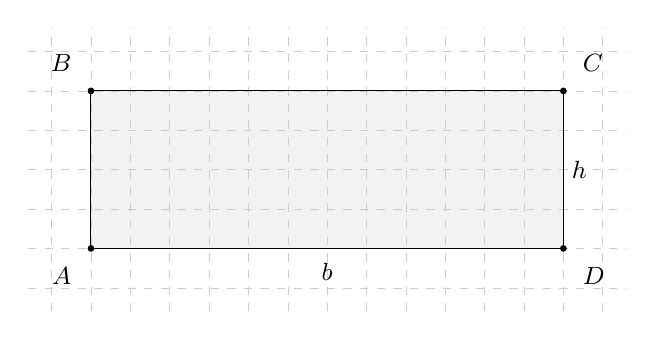
\begin{tikzpicture}[x=10mm,y=10mm,font=\small]

  \fill[fill=gray!10] (1,1) rectangle (7,3);
  \draw[style=help lines,step=5mm,dashed,black!20] (0.2,0.2) grid (7.8,3.8);
  \draw (1,1) rectangle (7,3);
  \node (b) at (4,.7) {$b$};
  \node (h) at (7.2,2) {$h$};
  \node [label={[name=label node]below left:$A$}] at (1,1) {};
  \node [label={[name=label node]above left:$B$}] at (1,3) {};
  \node [label={[name=label node]above right:$C$}] at (7,3) {};
  \node [label={[name=label node]below right:$D$}] at (7,1) {};

  \foreach \x in {1,7}
    \foreach \y in {1,3}
      \filldraw[fill=black, draw=black]  (\x,\y) circle (1pt);

\end{tikzpicture}

\end{center}

Come si può notare, per scrivere il risultato di un'operazione tra due numeri, in questo caso molto piccoli,
è necessario fare particolare attenzione in quanto, per l'eccessiva quantità di cifre decimali,
è facile commettere degli errori.

Per risolvere questo problema, si preferisce utilizzare una scrittura compatta che
permette di scrivere questo tipo di numeri in forma più agevole.
Una tale scrittura prende il nome di \emph{notazione scientifica}.

\begin{definizione}
Un numero~$\alpha$ è scritto in \emph{notazione scientifica} se
si presenta nella forma:
\[\alpha=k\cdot10^n\] 
dove~$k$ è un numero decimale maggiore o uguale a~$1$ e minore di~$10$ e~$n$ è un numero intero.
\end{definizione}

\begin{exrig}
 \begin{esempio}
I numeri~$\np{3,5e7}$ e~$\np{8,9e-5}$ sono scritti in notazione scientifica,
mentre i numeri~$\np{0,5e3}$ e~$\np{10,3e-8}$ non sono scritti in notazione scientifica
in quanto il numero davanti alla potenza di~$10$ nel primo caso è~$\np{0,5}$ che è minore di~$1$,
nel secondo caso è~$\np{10,3}$ che è maggiore di~$10$.
 \end{esempio}
\end{exrig}

\subsection{Come trasformare un numero in notazione scientifica}
Consideriamo la misura del diametro del globulo rosso, ovvero~$\np[m]{0,000007}$.
Per esprimere questa misura in notazione scientifica basta considerare la sua frazione generatrice, ovvero:
\[\np[m]{0,000007}=7\cdot\frac{1}{\np{1000000}}\unit{m}=\np[m]{7e-6}.\]

Allo stesso modo il numero~$\np{0,000000026}$ viene scritto in notazione scientifica come segue:
\[\np{0,000000026}=\np{2,6}\cdot\frac{1}{\np{100000000}}=\np{2,6}\cdot\frac{1}{10^8}=\np{2,6e-8}.\]
Si osservi che in questo secondo caso abbiamo preso in considerazione il valore~$\np{2,6}$ anziché~$26$, in quanto
il numero~$k$ deve essere minore di~$10$.

Consideriamo ora la misura del raggio della Terra, ovvero~$\np[m]{6400000}$,
la sua espressione in notazione scientifica sarà:~$\np{6,4e6}$.

Allo stesso modo il numero~$\np{340000000000}$ viene scritto in notazione scientifica~$\np{3,4e11}$.
Si osservi che in questo secondo caso abbiamo preso in considerazione il valore~$\np{3,4}$ anziché~$34$, in quanto,
come si è già detto, il numero~$k$ deve essere minore di~$10$.

\osservazione A numeri ``piccoli'', corrisponde una potenza di dieci con esponente negativo;
a numeri ``grandi'', corrisponde una potenza di dieci con esponente positivo.

\begin{procedura}
Scrivere un numero decimale positivo~$a$ in notazione scientifica, se~$a>1$:
\begin{enumeratea}
 \item si divide il numero decimale per una potenza di~$10$ in modo da avere un numero decimale compreso maggiore o uguale a~$1$ e minore di~$10$. Per trovare la potenza di~$10$ per la quale dividere il numero bisogna contare le cifre significative
del numero prima della eventuale virgola e togliere~$1$;
 \item per scrivere il numero~$a$ in notazione scientifica occorre moltiplicare il numero trovato al passo
precedente per la potenza di~$10$ utilizzata.
\end{enumeratea}
\end{procedura}

\begin{exrig}
 \begin{esempio}
Trasformare $\np{348000000000000}$ in notazione scientifica.
\begin{enumeratea}
\item Le cifre significative di~$\np{348000000000000}$ sono~$15$,
si divide quindi il numero per~$10^{14}$ e si ottiene~$\np{3,48}$;
\item $\np{3,48e14}$.
\end{enumeratea}
 \end{esempio}
\end{exrig}

\begin{procedura}
Scrivere un numero decimale positivo~$a$ in notazione scientifica, se~$0<a<1$:
\begin{enumeratea}
 \item si moltiplica il numero decimale per una opportuna potenza di~$10$ in modo da ottenere un numero maggiore o uguale a~$1$ e minore di~$10$. Per trovare la potenza di~$10$ bisogna contare gli zeri che si trovano tra la virgola e la prima cifra
significativa del numero e aggiungere~$1$;
 \item per scrivere il numero a in notazione scientifica occorre moltiplicare il numero ottenuto al passo
precedente per la stessa
potenza di~$10$ utilizzata presa però con esponente negativo.
\end{enumeratea}
\end{procedura}

\begin{exrig}
 \begin{esempio}
Trasformare $\np{0,000034}$ in notazione scientifica.
\begin{enumeratea}
\item Gli zero da considerare sono~$4$, si moltiplica allora il numero per~$10^5$ e si
ottiene~$3,4$;
\item quindi, per l'esempio considerato si ha~$\np{3,4e-5}$.
\end{enumeratea}
 \end{esempio}

\begin{esempio}
Riprendendo il problema della lamina rettangolare, le sue dimensioni in notazione scientifica vengono scritte come:
$b=\np[m]{6e-8}$, $h=\np[m]{2e-7}$.
L'area sarà quindi:
\begin{align*}
A =b\cdot h &=\np[m]{6e-8} \cdot \np[m]{2e-7}\\
 &=\np[m^2]{12e-15}\\
 &=\np{1,2}\cdot 10^1\cdot 10^{-15}\unit{m^2}\\
 &=\np[m^2]{1,2e-14}.
\end{align*}
Com'è possibile vedere, utilizzando le note proprietà delle potenze, si riesce ad eseguire l'operazione
in maniera molto agevole.
\end{esempio}

\begin{esempio}
Trasforma in notazione scientifica e calcola
$\displaystyle{\frac{\np{3000}:6\text{ milioni}}{\np{5000}\cdot\np{0,000002}}}$.

\begin{align*}
\frac{\np{3000}:6\text{ milioni}}{\np{5000}\cdot\np{0,000002}}&=\frac{(\np{3e3}):(\np{6e6})}{(\np{5e3})\cdot(\np{2e-6})}\\
 &=\frac{3:6\cdot10^{-3}}{5\cdot 2\cdot 10^{-3}}\\
 &=\frac{\np{0,5}}{10}\cdot10^{-3+3}\\
 &=\np{0,05}\cdot10^0\\
 &=\np{0,05}\\
 &=\np{5e-2}.
\end{align*}
\end{esempio}
\end{exrig}

\osservazione Un numero intero composto dalla cifra~1 seguita da un numero $n$ di cifre~0 può essere rappresentato più semplicemente come $10^n$.

\begin{exrig}
\begin{esempio}
 Potenze positive di 10.
\begin{multicols}{3}
\begin{enumeratea}
\item $10=10^1$;
\item $100=10^2$;
\item $\np{1000}=10^3$;
\item $\np{10000}=10^4$;
\item $\np{100000}=10^5$;
\item $\np{1000000}=10^6$;
\item $\np{10000000}=10^7$;
\item $\np{100000000}=10^8$;
\item $\np{1000000000}=10^9$.
\end{enumeratea}
\end{multicols}
\end{esempio}
\end{exrig}

\osservazione Un numero decimale con parte intera nulla seguita da $n$ cifre decimali tutte 0 tranne l'ultima che vale~1 può essere rappresentato più semplicemente come $10^{-n}$.

\begin{exrig}
\begin{esempio}
 Potenze negative di 10.
\begin{multicols}{3}
\begin{enumeratea}
\item $\np{0,1}=10^{-1}$;
\item $\np{0,01}=10^{-2}$;
\item $\np{0,001}=10^{-3}$;
\item $\np{0,0001}=10^{-4}$;
\item $\np{0,00001}=10^{-5}$;
\item $\np{0,000001}=10^{-6}$;
\item $\np{0,0000001}=10^{-7}$;
\item $\np{0,00000001}=10^{-8}$;
\item $\np{0,000000001}=10^{-9}$.
\end{enumeratea}
\end{multicols}

\end{esempio}
\end{exrig}

\ovalbox{\risolvii \ref{ese:3.66}, \ref{ese:3.67}, \ref{ese:3.68}, \ref{ese:3.69}, \ref{ese:3.70}, \ref{ese:3.71},
\ref{ese:3.72}, \ref{ese:3.73}}

\subsection{Ordine di grandezza}

Spesso, nel trattare i numeri molto grandi o molto piccoli, non è importante conoscere
la misura con precisione, ma basta conoscere ``quanto il valore è più o meno grande'',
cioè l'entità della sua grandezza. Per fare ciò si introduce il seguente concetto.

\begin{definizione}
Dato un numero, si definisce \emph{ordine di grandezza} (abbreviato con la sigla o.d.g.),
la potenza di~$10$ più vicina al numero.
\end{definizione}

Se un numero è equidistante dalle due potenze del 10 tra le quali è compreso, si assume come ordine di grandezza la potenza maggiore.

%\begin{procedura}
%Determinare l'ordine di grandezza di un numero:
%\begin{enumeratea}
%\item scrivi il numero dato in notazione scientifica~${k\cdot10^n}$;
%\item se~$k<5$ l'ordine di grandezza è~$10^n$;
%\item se~$k\ge5$ l'ordine di grandezza è~$10^{n+1}$.
%\end{enumeratea}
%\end{procedura}
%\newpage
\pagebreak
\begin{exrig}
 \begin{esempio}
Determinare l'ordine di grandezza dei numeri~$\np{0,000074}$ e~$\np{47000000000}$.

Scriviamo dapprima i numeri in notazione scientifica e poi l'o.d.g.
\begin{itemize}
  \item $\np{0,000074}=\np{7,4e-5}$.\quad L'o.d.g. è~$10^{-4}$ in quanto il numero~$7,4$ è maggiore di~$5$
  \item $\np{47000000000}=\np{4,7e10}$.\quad L'o.d.g. è~$10^{10}$ in quanto il numero~$4,7$ è minore di~$5$.
\end{itemize}
%\[\np{0,000074}=\np{7,4e-5}\quad\text{ e }\quad \np{47000000000}=\np{4,7e10}.\]
%L'o.d.g. del primo numero è~$10^{-4}$ in quanto il numero~$7,4$ è maggiore di~$5$.
%L'o.d.g. del secondo numero è~$10^{10}$ in quanto il numero~$4,7$ è minore di~$5$.
 \end{esempio}
\end{exrig}

\ovalbox{\risolvii \ref{ese:3.74}, \ref{ese:3.75}, \ref{ese:3.76}}

\section{Problemi con le frazioni}

\subsection{Problemi diretti}
Nei problemi diretti si conosce il valore di una grandezza e se ne deve calcolare la parte
che corrisponde a una frazione. In questo caso basta moltiplicare la
frazione per la grandezza intera.

\begin{exrig}
 \begin{esempio}
Una pasticceria produce~$568$ cornetti alla settimana: i~$3/4$ sono alla crema,~$1/8$ sono al cioccolato e
$1/8$ alla marmellata. Quanti cornetti di ciascun tipo produce?

Per risolvere il problema occorre calcolare la parte che corrisponde a ciascuna frazione:
\begin{itemize*}
\item cornetti alla crema:~$\dfrac{3}{4}\cdot 568 =426$;
\item cornetti al cioccolato:~$\dfrac{1}{8}\cdot 568 =71$;
\item cornetti alla marmellata (come per quelli al cioccolato):~$71$.
\end{itemize*}
 \end{esempio}
\end{exrig}

\subsection{Problemi inversi}

Nei problemi inversi si conosce il valore numerico di una frazione di una certa grandezza e
si deve calcolare il valore dell'intera grandezza.
In questo caso occorre dividere il valore numerico dato per la frazione, si ottiene così l'intero.

\begin{exrig}
 \begin{esempio}
Mario ha speso~\officialeuro~$21$ che corrispondono ai~$3/5$ della somma che possedeva. Quanto possedeva?

In questo problema si sa che \officialeuro~$21$ corrispondono ai~$3/5$ della somma da cercare.
Per trovare la somma posseduta da Mario è sufficiente dividere~$21$ per la frazione spesa, cioè
\officialeuro~$21$~$\displaystyle: 3/5=$ \officialeuro~$21\cdot 5/3=$ \officialeuro~$35$.
 \end{esempio}

 \begin{esempio}
Giuseppe possiede \officialeuro~$150$. Se spende i~$3/5$ della somma posseduta e poi i~$2/3$ della somma rimanente,
quanto gli rimane?

Per risolvere il problema si può procedere in più modi.

Calcoliamo prima i~$3/5$ di \officialeuro~$150$, cioè \officialeuro~$150\cdot 3/5=$ \officialeuro~$90$.
Quindi la prima volta Giuseppe spende \officialeuro~$90$, perciò gliene rimangono~$60$. La seconda volta spende
i~$2/3$ di \officialeuro~$60$, cioè \officialeuro~$60\cdot 2/3=$ \officialeuro~$40$. In tutto ha speso
\officialeuro~$90+$ \officialeuro~$40=$ \officialeuro~$130$ e quindi gli rimangono \officialeuro~$150-$ \officialeuro~$130=$ \officialeuro~$20$.

Un altro modo per risolvere il problema è tenere conto che,
se la prima volta ha speso i~$3/5$ della somma che possedeva,
significa che gli rimane la frazione~$1-3/5=2/5$.
La seconda volta spende i~$2/3$ dei~$2/5$ rimanenti, cioè~$\dfrac{2}{3}\cdot\dfrac{2}{5}=\dfrac{4}{15}$.
In tutto ha speso la frazione
\[\frac{3}{5}+\frac{4}{15}=\frac{3\cdot3+4}{15}=\frac{13}{15}\]
gli rimane perciò la frazione~$1-\dfrac{13}{15}=\dfrac{2}{15}$ ovvero \officialeuro~$150\cdot 2/15=$ \officialeuro~$20$.
 \end{esempio}
\end{exrig}

\ovalbox{\risolvii \ref{ese:3.77}, \ref{ese:3.78}, \ref{ese:3.79}, \ref{ese:3.80}}

\section{Le percentuali}

Avrai sentito parlare spesso che il prezzo di un oggetto è stato scontato del~$10$ per cento,
oppure che un partito politico ha preso il~$25$ per cento di voti
e altre espressioni simili che coinvolgono le percentuali.

Le percentuali sono un altro modo per scrivere le frazioni.

\begin{definizione}
Le \emph{percentuali} sono frazioni che hanno come denominatore~$100$ e come numeratore un numero intero o decimale.
\end{definizione}

La percentuale si indica con un numero intero o decimale seguita dal simbolo \%.
\[35\%=\frac{35}{100};\qquad7\%=\frac{7}{100};\qquad~\np{12,5}\%=\frac{\np{12,5}}{100}=\frac{125}{\np{1000}}.\]

Quindi, in generale
\begin{empheq}[box=\fbox]{equation*}
n\%=\frac{n}{100}
\end{empheq}

Per passare quindi dalla scrittura percentuale alla scrittura decimale basta dividere il
numero che esprime la percentuale per~$100$, cioè effettuare l'operazione di divisione tra il numeratore ed il denominatore:
\[35\%=\frac{35}{100}=\np{0,35};\qquad7\%=\frac{7}{100}=\np{0,07};\qquad\np{12,5}\%=\frac{\np{12,5}}{100}=\np{0,125}.\]

Per passare dalla scrittura decimale alla scrittura in percentuale, invece, occorre moltiplicare numeratore e denominatore per~$100$:
\[\np{0,02}=\frac{\np{0,02}}{1}=\frac{2}{100}=2\%;\qquad\np{0,23}=\frac{\np{0,23}}{1}=\frac{23}{100}=23\%;
\qquad\np{1,21}=\frac{\np{1,21}}{1}=\frac{121}{100}=121\%.\]

Per passare da una frazione alla sua scrittura in percentuale conviene prima scrivere la frazione come numero decimale e poi
da questo passare alla percentuale:
\[\frac{2}{3}=\np{0,}\overline6=\frac{\np{0,}\overline6}{1}=\frac{\np{66,}\overline6}{100}=\np{66,}\overline6\%.\]

\vspazio\ovalbox{\risolvii \ref{ese:3.81}, \ref{ese:3.82}, \ref{ese:3.83}, \ref{ese:3.84}}

\subsection{Problemi con le percentuali}

Per calcolare la percentuale di una grandezza è sufficiente moltiplicare il valore
della grandezza per la percentuale espressa in frazione.

\begin{exrig}
 \begin{esempio}
In una scuola che ha~$857$ alunni ne sono stati promossi il~$95$\%. Quanti sono stati i promossi?

Per rispondere, si moltiplica il numero totale di alunni per la frazione~$95/100$.
Precisamente~$\frac{95}{100}\cdot857=\np{814,15}$.
Poiché il risultato non è un numero intero, la percentuale è stata approssimata. Gli alunni promossi sono stati~$814$.
 \end{esempio}
\end{exrig}

A volte è nota una parte della grandezza e si vuole conoscere che percentuale è
la parte nota rispetto al totale. In questo caso occorre dividere la parte nota per l'intera grandezza,
moltiplicare il risultato per~$100$ ed esprimere il numero in percentuale.

\begin{exrig}
\begin{esempio}
Di una scolaresca di~$652$ alunni ben~$126$ hanno avuto il debito in matematica.
Qual è la percentuale di alunni che hanno avuto il debito in matematica?

Per rispondere alla domanda eseguiamo i seguenti calcoli:
\[\frac{126}{652}\cdot100\%\simeq\np{0,19}\cdot100\%=19\%.\]
\end{esempio}
\end{exrig}

Si noti che nell'ultimo esempio è stato utilizzato il simbolo $\simeq$ (\emph{circa uguale}) che indica un'approssimazione del calcolo, ovvero che la corrispondenza tra le scritture a sinistra e a destra di tale simbolo non è esatta, ma è approssimata all'ultima cifra decimale indicata nella scrittura di destra.

\subsection{Problemi con gli sconti}

\begin{exrig}
 \begin{esempio}
Un pantalone costava \officialeuro~$70$ e viene venduto con il~$20\%$ di sconto, a quanto viene venduto?

Si tratta di calcolare prima lo sconto e poi il prezzo scontato.
Lo sconto è dato da

\begin{center}
$20\%\cdot$ \officialeuro~$70=\dfrac{20}{100}\cdot$ \officialeuro~$70=$ \officialeuro~$14$.
\end{center}

Il prezzo scontato è \officialeuro~$70 -$ \officialeuro~$14=$ \officialeuro~$56$.

In alternativa si può tenere conto che, se~$20\%$ esprime lo sconto, la parte rimanente, quella da pagare, è
$100\%-20\%=80\%$. Quindi per calcolare quanto costano i pantaloni scontati si può calcolare

\begin{center}
$\displaystyle{80\%\cdot}$ \officialeuro~$70=\dfrac{80}{100}\cdot$ \officialeuro~$70=$ \officialeuro~56.
 \end{center}
 \end{esempio}

 \begin{esempio}
Un paio di scarpe da \officialeuro~$120$ viene venduto scontato a \officialeuro~$75$. Qual è stata la percentuale di
sconto praticato?

Per rispondere alla domanda, calcolo lo sconto \officialeuro~$120-$ \officialeuro~$75=$ \officialeuro~$45$.

Calcolo la percentuale che \officialeuro~$45$ rappresentano di \officialeuro~$120$,
\[\frac{45}{120}\cdot100\%=\np{0,375}\cdot100\%=\np{37,5}\%.\]
 \end{esempio}

\begin{esempio}
Mario ha trovato in un negozio il computer che stava cercando; per fortuna era scontato del~$15\%$ e così
ha risparmiato \officialeuro~$120$. Quanto costa il computer di listino?

Poiché \officialeuro~120 corrispondono al~$15\%$ del prezzo di listino, per calcolare il prezzo di listino occorre dividere~120 per la frazione che corrisponde a~$15\%$.
\begin{center}
	$120:~15\% =120:\dfrac{15}{100}=120\cdot\dfrac{100}{15}=$ \officialeuro~$800$.
\end{center}
\end{esempio}
\end{exrig}


\ovalbox{\risolvii \ref{ese:3.85}, \ref{ese:3.86}, \ref{ese:3.87}, \ref{ese:3.88}, \ref{ese:3.89}, \ref{ese:3.90},
\ref{ese:3.91}, \ref{ese:3.92}, \ref{ese:3.93}, \ref{ese:3.94}, \ref{ese:3.95}, \ref{ese:3.96},
\ref{ese:3.97},}

\vspazio\ovalbox{\ref{ese:3.98},\ref{ese:3.99}, \ref{ese:3.100}, \ref{ese:3.101}, \ref{ese:3.102}, \ref{ese:3.103}, \ref{ese:3.104},
\ref{ese:3.105}, \ref{ese:3.106}, \ref{ese:3.107}, \ref{ese:3.108}, \ref{ese:3.109}, \ref{ese:3.110}, \ref{ese:3.111},}

\vspazio\ovalbox{\ref{ese:3.112}, \ref{ese:3.113}, \ref{ese:3.114}, \ref{ese:3.115}, \ref{ese:3.116}}

\section{Proporzioni}

\begin{definizione}
 Il rapporto tra due numeri, di cui il secondo è diverso da zero, è il quoziente che si ottiene dividendo
il primo numero per il secondo. Il primo numero si dice \emph{antecedente}, il secondo \emph{conseguente}.
\end{definizione}

\begin{center}
  % (c) 2012 Dimitrios Vrettos - d.vrettos@gmail.com
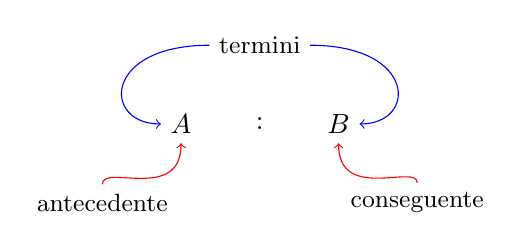
\begin{tikzpicture}[x=5mm,y=5mm]
  \node (a) at (-2,0) {$A$};
  \node (b) at (2,0) {$B$};
  \node (c) at (0,0) {$:$};
    \begin{scope}[font=\small]
    \node (ter) at (0,2) {termini};
    \node (ant) at (-4,-2) {antecedente};
    \node (con) at (4,-2) {conseguente};
    \end{scope}
    \begin{scope}[->]
      \begin{scope}[blue]
	\draw (ter) ..controls +(left:20mm) and +(left:10mm).. (a);
	\draw (ter) ..controls +(right:20mm) and +(right:10mm).. (b);
      \end{scope}
      \begin{scope}[red]
	\draw (ant) ..controls +(up:5mm) and +(down:10mm).. (a);
	\draw (con) ..controls +(up:5mm) and +(down:10mm).. (b);
      \end{scope}
    \end{scope}
\end{tikzpicture}

\end{center}

\begin{definizione}
 Una \emph{proporzione} è una uguaglianza tra due rapporti, del tipo
\[A: B = C: D\]
che si legge ``$A$ sta a~$B$ come~$C$ sta a~$D$'', con~$B$ e~$D$ diversi da zero. $A$ e~$D$ sono detti \emph{estremi}, mentre $B$ e~$C$ si dicono \emph{medi}.
\end{definizione}

\begin{center}
  % (c) 2012 Dimitrios Vrettos - d.vrettos@gmail.com

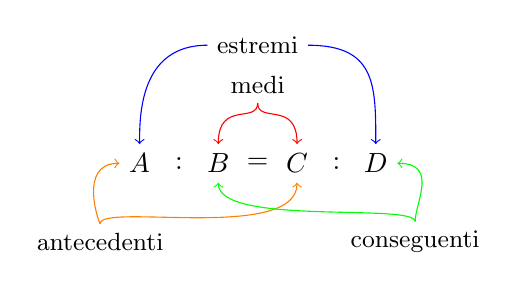
\begin{tikzpicture}[x=5mm,y=5mm]
  \node (a) at (-3,0) {$A$};
  \node (b) at (-1,0) {$B$};
  \node (e) at (0,0) {$=$};
  \node (c) at (1,0) {$C$};
  \node (d) at (3,0) {$D$};
  \foreach \x in {-2,2}
    \node (f) at (\x,0) {$:$};
  \begin{scope}[font=\small]
    \node (est) at (0,3) {estremi};
    \node (med) at (0,2) {medi};
    \node (ant) at (-4,-2) {antecedenti};
    \node (con) at (4,-2) {conseguenti};
  \end{scope}
  \begin{scope}[->]
    \begin{scope}[blue]
      \draw (est) ..controls +(left:15mm) and +(up:6mm).. (a);
      \draw (est) ..controls +(right:15mm) and +(up:10mm).. (d);
    \end{scope}
    \begin{scope}[red]
      \draw (med) ..controls +(down:5mm) and +(up:8mm).. (b);
      \draw (med) ..controls +(down:5mm) and +(up:8mm).. (c);
    \end{scope}
    \begin{scope}[orange]
      \draw (ant)..controls +(up:2mm) and +(left:8mm).. (a);
      \draw (ant)..controls +(up:5mm) and +(down:10mm).. (c);
    \end{scope}
    \begin{scope}[green]
      \draw (con)..controls +(up:5mm) and +(down:8mm).. (b);
      \draw (con)..controls +(up:5mm) and +(right:8mm).. (d);
    \end{scope}
  \end{scope}
\end{tikzpicture}

\end{center}

\begin{exrig}
\begin{esempio}
Determinare se quattro numeri sono in proporzione.
\begin{itemize*}
  \item $4:2=12:6$.\quad Formano una proporzione perché i due quozienti valgono entrambi~$2$;
  \item $7:14=16:4$.\quad \emph{Non} formano una proporzione perché il primo rapporto vale~$\np{0,5}$ mentre il secondo rapporto vale~$4$.
\end{itemize*}
\end{esempio}
\end{exrig}

%\begin{exrig}
% \begin{esempio}
%  $4:2=12:6$.
%
%Formano una proporzione perché i due quozienti valgono entrambi~$2$.
% \end{esempio}
%
%\begin{esempio}
%$7:14=16:4$.
%
% \emph{Non} formano una proporzione perché il primo rapporto vale~$\np{0,5}$ mentre il secondo rapporto vale~$4$.
%\end{esempio}
%\end{exrig}

\begin{proprieta}[Fondamentale delle proporzioni]
  In ogni proporzione il prodotto dei medi è uguale al prodotto degli estremi, cioè
\[A:B=C:D\quad\Rightarrow\quad A\cdot D=B\cdot C.\]
\end{proprieta}

\begin{exrig}
\begin{esempio}
Determinare se quattro numeri sono in proporzione.
\begin{itemize*}
  \item $4:6=6:9$ è una proporzione.
  
  Il prodotto dei medi è~$6\cdot6=36$ e il prodotto degli estremi è~$4\cdot9=36$. Quindi è una proporzione.
  \item $20:30=30:40$ non è una proporzione.
  
  Il prodotto dei medi è~$30\cdot30=900$ mentre il prodotto degli estremi è~$20\cdot40=800$. Quindi non è una proporzione.
\end{itemize*}
\end{esempio}
\end{exrig}
\begin{comment}
\begin{exrig}
 \begin{esempio}
Verificare se $4:6=6:9$ è una proporzione.

Il prodotto dei medi è~$6\cdot6=36$ e il prodotto degli estremi è~$4\cdot9=36$. Quindi è una proporzione.
 \end{esempio}

\begin{esempio}
Verificare se $20:30=30:40$ è una proporzione.

Il prodotto dei medi è~$30\cdot30=900$ mentre il prodotto degli estremi è~$20\cdot40=800$. Quindi non è una proporzione.
\end{esempio}
\end{exrig}
\end{comment}

\begin{proprieta}[del permutare]
  Se in una proporzione scambiamo tra loro i medi otteniamo ancora una proporzione;
in modo analogo otteniamo ancora una proporzione se scambiamo tra loro gli estremi,
o ancora se scambiamo tra loro sia i medi sia gli estremi, ovvero
\[A:B=C:D\quad\Rightarrow\quad A:C=B:D\quad\Rightarrow\quad D:B=C:A\quad\Rightarrow\quad D:C=B:A.\]
\end{proprieta}

\begin{exrig}
 \begin{esempio}
Data la proporzione~$12:16=18:24$ e scambiando tra loro:
\begin{itemize*}
  \item i medi si ottiene la proporzione~$12:18=16:24$;
  \item gli estremi si ottiene la proporzione~$24:16=18:12$;
  \item sia i medi che gli estremi si ottiene la proporzione~$24:18=16:12$.
\end{itemize*}

 \end{esempio}
\end{exrig}


\begin{proprieta}[dell'invertire]
  Se in una proporzione scambiamo ogni antecedente con il rispettivo conseguente
otteniamo ancora una proporzione, cioè
\[A:B=C:D\quad\Rightarrow\quad B:A=D:C.\]
\end{proprieta}

\begin{exrig}
 \begin{esempio}
Data la proporzione~$15:9=5:3$, applicando la proprietà dell'invertire
otteniamo la proporzione~$9:15=3:5$.
 \end{esempio}
\end{exrig}

\begin{proprieta}[del comporre]
  In una proporzione la somma dei primi due termini sta al primo termine come la
somma del terzo e del quarto termine sta al terzo termine. Analogamente,
la somma dei primi due termini sta al secondo termine come la somma del terzo e del quarto
termine sta al quarto termine. In termini matematici
\[A:B=C:D\quad\Rightarrow\quad (A+B):A=(C+D):C\phantom{.}\]
\[A:B=C:D\quad\Rightarrow\quad (A+B):B=(C+D):D.\]
\end{proprieta}
\pagebreak
\begin{exrig}
 \begin{esempio}
Data la proporzione~$16:10=40:25$, applicando la proprietà del comporre si ottengono le proporzioni
\[26:16=65:40\qquad\text{ e }\qquad26:10=65:25.\]
 \end{esempio}
\end{exrig}

Analogamente alla proprietà del comporre si ha la seguente:

\begin{proprieta}[dello scomporre]
  In una proporzione la differenza dei primi due termini sta al primo termine come la differenza del
 terzo e del quarto termine sta al terzo termine. Analogamente, la differenza dei primi due termini
sta al secondo termine come la differenza del terzo e del quarto termine sta al quarto termine. Quindi
\[A:B=C:D\quad\Rightarrow\quad (A-B):A=(C-D):C\phantom{.}\]
\[A:B=C:D\quad\Rightarrow\quad (A-B):B=(C-D):D.\]
\end{proprieta}

\begin{exrig}
 \begin{esempio}
Data la proporzione~$16:10=40:25$, applicando la proprietà dello scomporre si ottengono le proporzioni
\[6:16=15:40\qquad\text{ e }\qquad6:10=15:25.\]
 \end{esempio}
\end{exrig}

\subsection{Calcolo di un medio o un estremo incognito}
Il medio incognito di una proporzione si calcola moltiplicando gli estremi e dividendo per il medio noto:
\[a:b=x:d\quad\Rightarrow\quad x=\frac{a\cdot d}{b}.\]

L'estremo incognito di una proporzione si calcola moltiplicando i medi e dividendo per l'estremo noto:
\[x:b=c:d\quad\Rightarrow\quad x=\frac{b\cdot c}{d}.\]

\begin{exrig} %\vspace{-1ex}
\begin{esempio}
Calcola il termine incognito di ciascuna proporzione.
\vspace{-1.3ex}\begin{itemize*}
  \item $5:7=20:x\quad\Rightarrow\quad x=\frac{7\cdot 20}{5}=28$;
  \item $2:x=3:16\quad\Rightarrow\quad x=\frac{2\cdot 16}{3}=\frac{32}{3}$;
  \item $\frac{2}{3}:\frac{1}{2}=x:\frac{5}{6}%
\quad\Rightarrow\quad x=\frac{2}{3}\cdot\frac{5}{6}:\frac{1}{2}=\frac{2}{3}%
\cdot\frac{5}{6}\cdot\frac{2}{1}=\frac{10}{9}$.
\end{itemize*}
\end{esempio}%\vspace*{-1.7ex}
\end{exrig}

\begin{definizione}
  Una proporzione si dice \emph{continua} se ha i medi uguali.
\end{definizione}

Una proporzione continua è del tipo~$A:B=B:C$, per esempio le seguenti proporzioni sono continue
\[3:9=9:27\qquad5:10=10:20\qquad4:16=16:64.\]

\subsubsection*{Calcolo del medio in una proporzione continua}

In una proporzione continua il medio proporzionale incognito si ottiene moltiplicando gli estremi
e calcolando la radice quadrata del prodotto ottenuto, cioè
\[a:x=x:d\quad\Rightarrow\quad x=\sqrt{a\cdot d}.\]

\begin{exrig}
\begin{esempio}
Trova il valore di $x$ nella seguente proporzione continua~$36:x=x:9$.

\emph{Svolgimento}~$x=\sqrt{36\cdot 9}=18$.
\end{esempio}
\end{exrig}

\subsubsection*{Calcolo di un termine incognito per mezzo delle proprietà del comporre e dello scomporre}

\begin{exrig}
  \begin{esempio}
    Calcolare $x$ nella proporzione $(11-x):x=15:5$.

  Applicando la proprietà del comporre si ottiene la proporzione
  \begin{align*}
  (11-x+x):x=(15+5):5 &\:\Rightarrow\: 11:x=20:5\\
  &\:\Rightarrow\: x=\frac{11\cdot5}{20}=\frac{11}{4}.
  \end{align*}
  \end{esempio}

\begin{esempio}
 Calcolare $x$ nella proporzione $\displaystyle{\bigg(\frac{1}{2}+x\bigg):\frac{5}{8}=x:5}$.

 Permutando i medi si ha~$\displaystyle{\bigg(\frac{1}{2}+x\bigg):x=\frac{5}{8}:5}$.

 Applicando la proprietà dello scomporre si ha:
\begin{align*}
  &\bigg(\frac{1}{2}+x-x\bigg):x=\bigg(\frac{5}{8}-5\bigg):5\\
\Rightarrow\quad &\frac{1}{2}:x=\frac{-35}{8}:5\\
\Rightarrow\quad &x=\frac{1}{2}\cdot5:\bigg(\frac{-35}{8}\bigg)=\frac{1}{2}\cdot5%
\cdot\bigg(-\frac{8}{35}\bigg)=-\frac{4}{7}.
\end{align*}
\end{esempio}
\end{exrig}

\vspazio\ovalbox{\risolvii \ref{ese:3.117}, \ref{ese:3.118}, \ref{ese:3.119}, \ref{ese:3.120}, \ref{ese:3.121}, \ref{ese:3.122}, \ref{ese:3.123}, \ref{ese:3.124}}

\subsection{Grandezze direttamente e inversamente proporzionali}

Il perimetro di un triangolo equilatero varia al variare della lunghezza del suo lato.
Se si indica con~$l$ la lunghezza del lato del triangolo, allora il perimetro ($2p$) è dato dalla relazione:
\[2p=3\cdot l.\]

\begin{figure}[tbh]
\begin{minipage}[t]{.48\textwidth}
  \centering% (c) 2012 Dimitrios Vrettos - d.vrettos@gmail.com
\begin{tikzpicture}[domain=0:4.4,x=10mm,y=5mm]
  \draw[->] (0,0) -- coordinate (x axis mid) (5.2,0) node [right] () {$x$}; % asse x
  \draw[->] (0,0) -- coordinate (y axis mid) (0,14.5) node [above] () {$y$}; % asse y
%  \draw[->] (0,0) -- coordinate (x axis mid) (5.2,0)}; % asse x
%  \draw[->] (0,0) -- coordinate (y axis mid) (0,14.5); % asse y
  % etichette
  \foreach \x in {0,1,...,5}
    \draw (\x,3pt) -- (\x,-3pt) node[anchor=north] {\x};
  \foreach \y in {1,2,...,14}
    \draw (3pt,\y) -- (-3pt,\y) node[anchor=east] {\y}; 
  \draw (3pt,0) -- (-3pt,0); 
  \node[below=0.5cm] at (x axis mid) {lato $l$};
  \node[rotate=90,above left=1cm] at (y axis mid) {perimetro $2p$};
  %grafico
  \draw[color=blue] plot  (\x,{3*\x});
  \begin{scope}[dotted]
    \foreach \x in {1,2,3,4}{
      \draw (\x,0) -- (\x,3*\x);
      \draw (0,3*\x) -- (\x,3*\x);
    }
  \end{scope}
\end{tikzpicture}

  \caption{Proporzionalità diretta.}\label{fig:3.2}  
\end{minipage}\hfil
 \begin{minipage}[t]{.48\textwidth}  
 \centering% (c) 2012 Dimitrios Vrettos - d.vrettos@gmail.com
\begin{tikzpicture}[x=10mm,y=10mm, smooth]
  \draw[->] (0,0) -- coordinate (x axis mid) (5.2,0) node [right] () {$x$};
  \draw[->] (0,0) -- coordinate (y axis mid) (0,4.5) node [above] () {$y$};
  \foreach \x in {0,1,...,5}
    \draw (\x,3pt) -- (\x,-3pt) node[anchor=north] {\x};
  \foreach \y in {1,2,...,4.5}
    \draw (3pt,\y) -- (-3pt,\y) node[anchor=east] {\y}; 
  \draw (3pt,0) -- (-3pt,0);
  %labels      
  \node[below=0.5cm] at (x axis mid) {volume $V$};
  \node[rotate=90,above left=1cm] at (y axis mid) {pressione $P$};
  \draw[domain=.5:4.4,color=blue] plot  (\x,{2/\x});
  \begin{scope}[dotted]
    \foreach \x in {.5,1,2,3,4.4}{
      \draw (\x,0) -- (\x,2/\x);
      \draw (0,2/\x) -- (\x,2/\x);
    }
  \end{scope}
\end{tikzpicture}

 \caption{Proporzionalità inversa.}\label{fig:3.3}
 \end{minipage}
\end{figure}

È possibile notare che se si raddoppia il lato, raddoppia anche il perimetro; se si triplica il lato,
allora triplica anche il perimetro, ecc.
\begin{center}
 \begin{tabular*}{.75\textwidth}{l@{\extracolsep{\fill}}*{6}{c}}
\toprule
Lato~($l$)               &$\np{0,5}$&$1$&$\np{1,5}$&$\np{2,4}$&$\np{3,1}$&$\np{4,4} $\\
Perimetro~($2p$)         &$\np{1,5}$&$3$&$\np{4,5}$&$\np{7,2}$&$\np{9,3}$&$\np{13,2}$\\
Rapporto~$\dfrac{2p}{l}$ &$    3   $&$3$&$    3   $&$   3    $&$   3    $&$    3    $\\
\bottomrule
\end{tabular*}
\end{center}

\begin{definizione}
  Due grandezze~$x$ e~$y$ si dicono \emph{direttamente proporzionali} se il loro rapporto è costante, cioè
\[\frac{y}{x}=k\text{,~~con }k\neq~0.\]
\end{definizione}

In generale, da quest'ultima scrittura, possiamo dedurre che una proporzionalità diretta è
espressa da una formula del tipo:
\[y=kx\text{,~~con }k\neq 0.\]

Graficamente un tale tipo di proporzionalità è rappresentato da una retta che
passa per l'origine di un sistema di assi cartesiani ortogonali (figura~\ref{fig:3.2}).

Esaminiamo ora un altro esempio. Se quando vai a fare benzina allo scooter chiedi ogni volta \officialeuro~$10$ di benzina,
 noterai che se aumenta il prezzo della benzina diminuirà la quantità di carburante che ricevi e viceversa
se diminuisce il prezzo aumenterà la quantità di carburante che ricevi. Ciò che rimane costante è il prodotto
tra il prezzo della benzina e la quantità di benzina ricevuta che deve essere sempre \officialeuro~$10$.
\begin{center}
 \begin{tabular*}{.8\textwidth}{l@{\extracolsep{\fill}}*{4}{c}}
\toprule
Prezzo benzina al litro:~$p$ (\officialeuro) &$\np{1,126}$&$\np{1,156}$&$\np{1,212}$&$\np{1,248}$\\
Benzina ricevuta:~$b$ (l)                    &$\np{8,881}$&$\np{8,650}$&$\np{8,251}$&$\np{8,013}$\\
Costo:~$c=p\cdot b$ (\officialeuro)          &$\np{10,00}$&$\np{10,00}$&$\np{10,00}$&$\np{10,00}$\\
\bottomrule
\end{tabular*}
\end{center}

\begin{definizione}
  Due grandezze~$x$ e~$y$ si dicono \emph{inversamente proporzionali} se il loro prodotto è costante,
cioè
\[x\cdot y=k\text{,~~con }k\neq 0.\]
\end{definizione}

In generale, da quest'ultima scrittura, possiamo dedurre che una proporzionalità inversa è
espressa da una formula del tipo:
\[y=\frac{k}{x}\text{,~~con }k\neq~0.\]

Graficamente un tale tipo di proporzionalità è rappresentato, in un sistema di assi cartesiani ortogonali, da un ramo d'iperbole
equilatera (figura~\ref{fig:3.3}).

\vspazio\ovalbox{\risolvii \ref{ese:3.125}, \ref{ese:3.126}, \ref{ese:3.127}, \ref{ese:3.128}}

\section{Espressioni con le frazioni}
\begin{exrig}
\begin{esempio}
%\begin{problema}
  Calcola il valore della seguente espressione.
\[  \bigg\lbrace\frac{3}{20}\cdot\bigg[\bigg(\frac{4}{9}-\frac{1}{3}\bigg):5+ \bigg(\frac{3}{7}-\frac{2}{5}\bigg):%
\frac{1}{14}+\frac{1}{5}\cdot\frac{1}{9}\bigg]+\frac{2}{15}\bigg\rbrace:2.\]
%\end{problema}
%\begin{soluzione}
\begin{align*}
  \bigg\lbrace\frac{3}{20}\cdot\bigg[\bigg(\frac{4}{9}-\frac{1}{3}\bigg):5 + \bigg(\frac{3}{7}-\frac{2}{5}\bigg):&%
\frac{1}{14}+\frac{1}{5}\cdot\frac{1}{9}\bigg]+\frac{2}{15}\bigg\rbrace:2= \\
=&
\bigg\lbrace\frac{3}{20}\cdot\bigg[\bigg(\frac{4-3}{9}\bigg):5+\bigg(\frac{15-14}{35}\bigg):\frac{1}{14}+\frac{1}{45}\bigg]%
+\frac{2}{15}\bigg\rbrace:2\\
=&
\bigg\lbrace\frac{3}{20}\cdot\bigg[\frac{1}{9}:5+\frac{1}{35}:\frac{1}{14}+\frac{1}{45}\bigg]+\frac{2}{15}\bigg\rbrace:2\\
=&
\bigg\lbrace\frac{3}{20}\cdot\bigg[\frac{1}{9}\cdot\frac{1}{5}+\frac{1}{35}\cdot\frac{14}{1}+\frac{1}{45}\bigg]+\frac{2}{15}\bigg\rbrace:2\\
=&
 \bigg\lbrace\frac{3}{20}\cdot\bigg[\frac{1}{45}+\frac{14}{35}+\frac{1}{45}\bigg]+%
 \frac{2}{15}\bigg\rbrace:2\\
=&
\bigg\lbrace\frac{3}{20}\cdot\bigg[\frac{1}{45}+\frac{2}{5}+\frac{1}{45}\bigg]+\frac{2}{15}\bigg\rbrace:2\\
=&
\bigg\lbrace\frac{3}{20}\cdot\bigg[\frac{1+18+1}{45}\bigg]+\frac{2}{15}\bigg\rbrace:2\\
=&
\bigg\lbrace\frac{3}{20}\cdot\frac{20}{45}+\frac{2}{15}\bigg\rbrace:2\\
=&
\bigg\lbrace\frac{3}{45}+\frac{2}{15}\bigg\rbrace:2\\
=&
\bigg\lbrace\frac{1}{15}+\frac{2}{15}\bigg\rbrace:2\\
=&
\frac{3}{15}:2\\
=&
\frac{1}{5}\cdot\frac{1}{2}=\frac{1}{10}.
\end{align*}
%\end{soluzione}
\end{esempio}

\begin{esempio}
  Calcola il valore della seguente espressione.
\[\bigg[\frac{1}{4}\cdot\frac{5}{2}-\bigg(\frac{3}{5} - \frac{1}{2}\bigg)\cdot\frac{25}{4}\bigg]\cdot\bigg[\bigg(\frac{5}{8}-\frac{4}{5}\bigg)\cdot\frac{8}{3}-\frac{15}{4}:\bigg(\frac{8}{3}-1\bigg)+\frac{10}{3}\bigg].\]
  \begin{align*}
\bigg[\frac{1}{4}\cdot\frac{5}{2}-\bigg(\frac{3}{5} - \frac{1}{2}\bigg)\cdot\frac{25}{4}\bigg]\cdot\bigg[\bigg(&\frac{5}{8}-\frac{4}{5}\bigg)\cdot\frac{8}{3}-\frac{15}{4}:\bigg(\frac{8}{3}-1\bigg)+\frac{10}{3}\bigg]=\\
&=\bigg[\frac{5}{8}-\bigg(\frac{6-5}{10}\bigg)\cdot\frac{25}{4}\bigg]\cdot\bigg[\bigg(\frac{25-32}{40}\bigg)\cdot\frac{8}{3}-\frac{15}{4}:\bigg(\frac{8-3}{3}\bigg)+\frac{10}{3}\bigg]\\
&=\bigg[\frac{5}{8}-\frac{1}{10}\cdot\frac{25}{4}\bigg]\cdot\bigg[-\frac{7}{40}\cdot\frac{8}{3}-\frac{15}{4}:\frac{5}{3}+\frac{10}{3}\bigg]\\
&=\bigg[\frac{5}{8}-\frac{5}{8}\bigg]\cdot\bigg[-\frac{7}{15}-\frac{15}{4}\cdot\frac{3}{5}+\frac{10}{3}\bigg]\\
&=0\cdot\bigg[-\frac{7}{15}-\frac{9}{4}+\frac{10}{3}\bigg]\\
&=0.
  \end{align*}
\end{esempio}

\begin{esempio}
%\begin{problema}
  Calcola il valore della seguente espressione.
\[\bigg[\frac{13}{5}:\bigg(3+\frac{9}{10}\bigg)+\frac{7}{8}+\bigg(\frac{13}{4}-2\bigg)\cdot\frac{4}{15}-\frac{7}{8}%
\bigg]\cdot\frac{11}{3}:\bigg(6-\frac{1}{2}\bigg).\]
%\end{problema}
%\begin{soluzione}
  \begin{align*}
\bigg[\frac{13}{5}:\bigg(3+\frac{9}{10}\bigg)+\frac{7}{8}+\bigg(\frac{13}{4}-&2\bigg)\cdot\frac{4}{15}-\frac{7}{8}%
\bigg]\cdot\frac{11}{3}:\bigg(6-\frac{1}{2}\bigg)=\\
&=
\bigg[\frac{13}{5}:\bigg(\frac{30+9}{10}\bigg)+\frac{7}{8}+\bigg(\frac{13-8}{4}\bigg)\cdot\frac{4}{15}-\frac{7}{8}%
\bigg]\cdot\frac{11}{3}:\bigg(\frac{12-1}{2}\bigg)\\
 &=
\bigg[\frac{13}{5}:\frac{39}{10}+\frac{7}{8}+\frac{5}{4}\cdot\frac{4}{15}-\frac{7}{8}%
\bigg]\cdot\frac{11}{3}:\frac{11}{2}\\
 &=
\bigg[\frac{13}{5}\cdot\frac{10}{39}+\frac{7}{8}+\frac{1}{3}-\frac{7}{8}%
\bigg]\cdot\frac{11}{3}\cdot\frac{2}{11}\\
 &=
\bigg[\frac{2}{3}+\frac{7}{8}+\frac{1}{3}-\frac{7}{8}%
\bigg]\cdot\frac{2}{3}\\
 &=
\bigg[\frac{2}{3}+\frac{1}{3}\bigg]\cdot\frac{2}{3}\\
&=1\cdot\frac{2}{3}\\
&=\frac{2}{3}.
  \end{align*}
%\end{soluzione}
\end{esempio}
\pagebreak
\begin{esempio}
%\begin{problema}
   Calcola il valore della seguente espressione.
\[\bigg[\bigg(\frac{7}{5}-\frac{1}{2}\bigg)^{2}:\bigg(\frac{9}{10}\bigg)^{2}-\bigg(1+\frac{2}{3}-2\bigg)^{2}\bigg]^{2}:\bigg(\frac{10}{9}\bigg)^{2}-\bigg(1+\frac{8}{5}+\frac{1}{25}\bigg).\]
% \end{problema}

%\begin{soluzione}
 \begin{align*}
\bigg[\bigg(\frac{7}{5}-\frac{1}{2}\bigg)^{2}:\bigg(\frac{9}{10}\bigg)^{2}-&\bigg(1+\frac{2}{3}-2\bigg)^{2}\bigg]^{2}:%
\bigg(\frac{10}{9}\bigg)^{2}-\bigg(1+\frac{8}{5}+\frac{1}{25}\bigg)=\\
=&\bigg[\bigg(\frac{14-5}{10}\bigg)^{2}:\bigg(\;\frac{9}{10}\bigg)^{2}-\bigg(\frac{3+2-6}{3}\bigg)^{2}\bigg]^{2}:%
\bigg(\frac{10}{9}\bigg)^{2}-\bigg(\frac{25+40+1}{25}\bigg)\\
=&\bigg[\bigg(\;\frac{9}{10}\bigg)^{2}:\bigg(\;\frac{9}{10}\bigg)^{2}-\bigg(-{\frac{1}{3}}\bigg)^{2}\bigg]^{2}:\bigg(\frac{10}{9}\bigg)^{2}-\frac{66}{25}\\
=&\bigg[1-\frac{1}{9}\bigg]^{2}:\bigg(\frac{10}{9}\bigg)^{2}-\frac{66}{25}\\
=&\bigg[\frac{8}{9}\bigg]^{2}\cdot\bigg(\frac{9}{10}\bigg)^{2}-\frac{66}{25}\\
=&\bigg(\frac{4}{5}\bigg)^{2}-\frac{66}{25}\\
=&\frac{16}{25}-\frac{66}{25}\\
=&-{\frac{50}{25}}\\
=&-2.
\end{align*}
%\end{soluzione}
\end{esempio}
\end{exrig}

\vspazio\ovalbox{\risolvii \ref{ese:3.129}, \ref{ese:3.130}, \ref{ese:3.131}, \ref{ese:3.132}, \ref{ese:3.133}, \ref{ese:3.134}, \ref{ese:3.135}, \ref{ese:3.136}, \ref{ese:3.137}, \ref{ese:3.138}, \ref{ese:3.139}}

\newpage
% (c)~2012 Dimitrios Vrettos - d.vrettos@gmail.com
\section{Esercizi}
\subsection{Esercizi dei singoli paragrafi}
\subsubsection*{3.2 - Frazioni}

\begin{esercizio}[\Ast]
\label{ese:3.1}
Da un cartoncino rettangolare quadrettato di lati rispettivamente~5 unità e~8~unità viene ritagliata
la forma colorata in grigio, come mostrato nella figura di seguito riportata.
\begin{center}
 % (c) 2012 Dimitrios Vrettos - d.vrettos@gmail.com
% Esercizio 3.1

\begin{tikzpicture}
\draw[step=5mm, black] (0,0) grid (40mm,25mm);

\fill[gray, opacity=.4] (10mm,5mm) rectangle (15mm,10mm);
\fill[gray, opacity=.4] (25mm,5mm) rectangle (35mm,10mm);
\fill[gray, opacity=.4] (10mm,10mm) rectangle (30mm,15mm);
\fill[gray, opacity=.4] (5mm,15mm) rectangle (30mm,20mm);

\draw[|-|] (0,26.5mm) -- (40mm,26.5mm);
\node (8u) at (20mm,30mm) {$8\text{ unità}$};

\draw[|-|] (41.5mm,0) -- (41.5mm,25mm);
\node[rotate=-90] (5u) at (45mm,12.5mm) {$5\text{ unità}$};
\end{tikzpicture}

\end{center}
Quale frazione rappresenta il rapporto tra la forma ritagliata e il cartoncino?
\end{esercizio}

\begin{esercizio}
\label{ese:3.2}
Il monte-premi di una lotteria è di \officialeuro~$\np{50000}$. Il primo premio è di \officialeuro~$\np{25000}$, il secondo di
\officialeuro~$\np{10000}$, il terzo di \officialeuro~$\np{5000}$, il quarto di \officialeuro~$\np{4000}$, il quinto e il sesto premio sono uguali.
Nella figura un quadretto rappresenta \officialeuro~$\np{1000}$ ed il totale è il monte-premi.
\begin{center}
 % (c) 2012 Dimitrios Vrettos - d.vrettos@gmail.com
% Esercizio 3.2

\begin{tikzpicture}
\draw[step=5mm, black] (0,0) grid (50mm,25mm);
\end{tikzpicture}

\end{center}
\begin{enumeratea}
 \item Colora con colori diversi i quadretti che servono per rappresentare i sei premi, un colore per ogni premio;
 \item quale parte del monte-premi è stata incassata da chi ha vinto il secondo premio?
	Esprimi questa parte con una frazione;
 \item Marco ha vinto il sesto premio: quanto ha vinto?
\end{enumeratea}
\end{esercizio}

\begin{esercizio}[\Ast]
 \label{ese:3.3}
La figura seguente è composta da~$11$ quadratini, alcuni bianchi altri grigi.
\begin{center}
 % (c) 2012 Dimitrios Vrettos - d.vrettos@gmail.com
% Esercizio 3.3
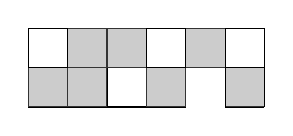
\begin{tikzpicture}
  \begin{scope}[step=5mm, black]
    \draw (0,0) grid (20mm,10mm);
    \draw (20mm,5mm) grid (25mm,10mm);
    \draw (25mm,0) grid (30mm,10mm);
  \end{scope}
  \begin{scope}[gray, opacity=.4]
    \fill (0,0) rectangle (10mm,5mm);
    \fill (15mm,0) rectangle (20mm,5mm);
    \fill (25mm,0) rectangle (30mm,5mm);
    \fill (5mm,5mm) rectangle (15mm,10mm);
    \fill (20mm,5mm) rectangle (25mm,10mm);   
  \end{scope}
  \draw (25mm,0)--(25mm,5mm);
\end{tikzpicture}

\end{center}
Quale frazione rappresenta la parte grigia rispetto all'intera figura? Quale frazione la parte bianca?
\end{esercizio}
\pagebreak
\begin{esercizio}
 \label{ese:3.4}
 Di ciascuna figura colora la parte indicata dalla frazione.
\begin{center}
 % (c) 2012 Dimitrios Vrettos - d.vrettos@gmail.com
% Esercizio 3.4

\begin{tikzpicture}

\draw  (0,0) circle(.8cm);
\draw (1.8cm,-.8cm) rectangle (4.1cm,.8cm);
\node [star, star point height=.5cm, minimum size=1.8cm, rotate=45, draw] at (5.9cm,0) {};

\node (cercio) at (0,1.5cm) {$\displaystyle\frac{3}{5}$};
\node (rettangolo) at (2.95cm,1.5cm) {$\displaystyle\frac{2}{3}$};
\node (cercio) at (5.9cm,1.5cm) {$\displaystyle\frac{1}{2}$};
\end{tikzpicture}

\end{center}
\end{esercizio}

\begin{esercizio}
\label{ese:3.5}
 Indica se le frazioni sono proprie (P), improprie (I) o apparenti (A).
 \begin{multicols}{3}
 \TabPositions{0.6cm}
 \begin{enumeratea}
 \item $\dfrac{3}{4}$ \tab\quad\boxP\quad\boxI\quad\boxA\vspace{1.1ex}
 \item $\dfrac{8}{3}$ \tab\quad\boxP\quad\boxI\quad\boxA
 \item $\dfrac{12}{3}$ \tab\quad\boxP\quad\boxI\quad\boxA\vspace{1.1ex}
 \item $\dfrac{5}{2}$ \tab\quad\boxP\quad\boxI\quad\boxA
 \item $\dfrac{5}{3}$ \tab\quad\boxP\quad\boxI\quad\boxA\vspace{1.1ex}
 \item $\dfrac{3}{2}$ \tab\quad\boxP\quad\boxI\quad\boxA
 \end{enumeratea}
 \end{multicols}
\end{esercizio}

\begin{esercizio}
\label{ese:3.6}
Trova le frazioni equivalenti completando.
 \begin{multicols}{4}
 \begin{enumeratea}
 	\item $\dfrac{3}{4}=\dfrac{\ldots}{12}$;
 	\item $\dfrac{12}{16}=\dfrac{3}{\ldots}$;
 	\item $\dfrac{5}{2}=\dfrac{\ldots}{10}$;
 	\item $\dfrac{21}{35}=\dfrac{\ldots}{5}$.
 \end{enumeratea}
 \end{multicols}
\end{esercizio}

\begin{esercizio}
\label{ese:3.7}
Sottolinea le frazioni equivalenti a~$\dfrac{3}{5}$ tra le seguenti.
\[\frac{6}{10};\qquad\frac{25}{100};\qquad\frac{12}{10};\qquad\frac{5}{25}.\]
\end{esercizio}

\begin{esercizio}
\label{ese:3.8}
Completa le seguenti uguaglianze.
\begin{multicols}{4}
\begin{enumeratea}
\item $\displaystyle{\frac{3}{5}=\frac{\ldots}{10}}$;
\item $\displaystyle{\frac{75}{10}=\frac{\ldots}{100}}$;
\item $\displaystyle{\frac{7}{\ldots}=\frac{1}{2}}$;
\item $\displaystyle{3=\frac{24}{\ldots}}$.
\end{enumeratea}
\end{multicols}
\end{esercizio}

\begin{esercizio}
 \label{ese:3.9}
 Indica almeno tre frazioni equivalenti a ciascuna delle seguenti.
 \begin{multicols}{6}
 \begin{enumeratea}
 	\item $\dfrac{5}{6}$;
 	\item $\dfrac{3}{5}$;
 	\item $\dfrac{12}{60}$;
 	\item $\dfrac{2}{3}$;
 	\item $\dfrac{1}{2}$;
 	\item $\dfrac{5}{2}$.
 \end{enumeratea}
 \end{multicols}
\end{esercizio}

\begin{esercizio}
 \label{ese:3.10}
Nella figura che segue il quadratino colorato rappresenta~$1/4$ del quadrato grande; costruisci una figura
che rappresenti~$8/4$ del quadrato grande accostando opportunamente altri quadrati uguali.
 \begin{center}
 % (c) 2012 Dimitrios Vrettos - d.vrettos@gmail.com
% Quadrato 1/4
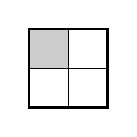
\begin{tikzpicture}
  \begin{scope}[scale=1,every node/.style={minimum size=5mm}]
    \draw[step=5mm, black] (0,0) grid (1,1);
    \fill[gray, opacity=.4] (0,.5) rectangle (.5,1);
    \draw[black,thick] (0,0) rectangle (1,1);
  \end{scope} 
\end{tikzpicture}

 \end{center}
\end{esercizio}

\begin{esercizio}
 \label{ese:3.11}
Riduci ai minimi termini le seguenti frazioni.
 \begin{multicols}{6}
 \begin{enumeratea}
 \item $\dfrac{4}{6}$;\vspace{1.1ex}
 \item $\dfrac{8}{2}$;\vspace{1.1ex}
 \item $\dfrac{2}{10}$;
 \item $\dfrac{18}{16}$;\vspace{1.1ex}
 \item $\dfrac{3}{12}$;\vspace{1.1ex}
 \item $\dfrac{6}{20}$;
 \item $\dfrac{80}{100}$;\vspace{1.1ex}
 \item $\dfrac{8}{12}$;\vspace{1.1ex}
 \item $\dfrac{9}{6}$;
 \item $\dfrac{10}{15}$;\vspace{1.1ex}
 \item $\dfrac{14}{49}$;\vspace{1.1ex}
 \item $\dfrac{15}{21}$.
 \end{enumeratea}
 \end{multicols}
\end{esercizio}

\begin{esercizio}
 \label{ese:3.12}
Riduci ai minimi termini le seguenti frazioni.
 \begin{multicols}{6}
 \begin{enumeratea}
 \item $\dfrac{16}{6}$;\vspace{1.1ex}
 \item $\dfrac{18}{15}$;\vspace{1.1ex}
 \item $\dfrac{20}{12}$;
 \item $\dfrac{21}{9}$;\vspace{1.1ex}
 \item $\dfrac{24}{30}$;\vspace{1.1ex}
 \item $\dfrac{25}{15}$;
 \item $\dfrac{27}{21}$;\vspace{1.1ex}
 \item $\dfrac{28}{14}$;\vspace{1.1ex}
 \item $\dfrac{30}{16}$;
 \item $\dfrac{32}{24}$;\vspace{1.1ex}
 \item $\dfrac{35}{10}$;\vspace{1.1ex}
 \item $\dfrac{36}{81}$;
 \item $\dfrac{40}{6}$;\vspace{1.1ex}
 \item $\dfrac{42}{21}$;\vspace{1.1ex}
 \item $\dfrac{45}{27}$;
 \item $\dfrac{48}{60}$;\vspace{1.1ex}
 \item $\dfrac{12}{30}$;\vspace{1.1ex}
 \item $\dfrac{135}{77}$.
% \item $\dfrac{121}{22}$;\vspace{1.1ex}
% \item $\dfrac{87}{99}$;\vspace{1.1ex}
% \item $\dfrac{15}{360}$;
% \item $\dfrac{110}{30}$;\vspace{1.1ex}
% \item $\dfrac{240}{75}$;\vspace{1.1ex}
% \item $\dfrac{140}{294}$.
 \end{enumeratea}
 \end{multicols}
\end{esercizio}

\begin{figure}[t]
 \begin{minipage}[b]{.45\textwidth}
 \centering% (c) 2012 Dimitrios Vrettos - d.vrettos@gmail.com
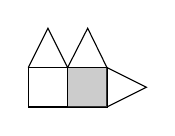
\begin{tikzpicture}
\draw (0,0) rectangle  (10mm,5mm);
\draw (0,5mm) -- (2.5mm,10mm)--(5mm,5mm)--(7.55mm,10mm)--(10mm,5mm);
\draw (10mm,5mm) -- (15mm,2.5mm)--(10mm,0);
\draw (5mm,0) -- (5mm,5mm);

\fill[gray, opacity=.4](5mm,0) rectangle  (10mm,5mm);
\end{tikzpicture}

\caption{}\label{fig:3.4}
 \end{minipage}\hfil
\begin{minipage}[b]{.45\textwidth}
 \centering% (c) 2012 Dimitrios Vrettos - d.vrettos@gmail.com
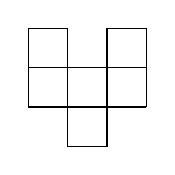
\begin{tikzpicture}
\draw[step=5mm] (0,0) grid  (15mm,5mm);
\draw (0,5mm) rectangle  (5mm,10mm);
\draw (10mm,5mm) rectangle  (15mm,10mm);
\draw (5mm,0) rectangle  (10mm,-5mm);
\end{tikzpicture}

 \caption{}\label{fig:3.5}
 \end{minipage}
\end{figure}

\begin{esercizio}
 \label{ese:3.13}
Si può dire che la parte colorata in grigio della figura \ref{fig:3.4} corrisponde a~$\frac{1}{5}$ della figura stessa?
\end{esercizio}

\begin{esercizio}
 \label{ese:3.14}
Costruisci una figura che corrisponde a~$\frac{11}{6}$ della figura \ref{fig:3.5}.
\end{esercizio}

\begin{esercizio}
 \label{ese:3.15}
Per quali dei seguenti disegni la parte colorata in grigio rappresenta sempre la frazione~$\dfrac{3}{4}$
del quadrato bianco?
 \begin{center}
 % (c) 2012 Dimitrios Vrettos - d.vrettos@gmail.com

\begin{tikzpicture}
  \begin{scope}[x=25mm,y=5mm]
    % Costruzione dei 5 quadrati
    \foreach \x in {0,1,...,4}
      \node[draw, minimum size=20mm](quad) at(\x,0) {};
    %  Nomi
%     \foreach \c [count=\x from 0] in {$A$,$B$,$C$,$D$,$E$} 
%       \node[below=13mm] at (\x,0) {\c};
    %  quadrato B
    \draw(15mm,2)--(1,-2);
    \draw(1,-2)--(35mm,2);
    \draw(1,-2)--(1,2);
    \begin{scope}[fill=gray, fill opacity=.4]
      \fill (15mm,2)--(1,2)--(1,-2);
      \fill (1,-2) rectangle (35mm,2);
    \end{scope}
    % quadrato C
    \draw(40mm,2)--(60mm,-2);
    \draw (40mm,-2) -- (60mm,2);
    \begin{scope}[fill=gray, fill opacity=.4]
      \fill (40mm,2)--(60mm,-2)--(40mm,-2);
      \fill (60mm,2)--(60mm,-2)--(2,0);
    \end{scope}
    % quadrato D
    \draw (65mm,0) -- (85mm,0);
    \draw (3,-2) -- (3,2);
    \begin{scope}[fill=gray, fill opacity=.4]
      \fill (65mm,-2) rectangle (3,2);
      \fill (3,-2) rectangle (85mm,0);
    \end{scope}
    % quadrato E
    \foreach \y in {-1,0,1}
      \draw (90mm,\y) -- (110mm,\y);
    \begin{scope}[fill=gray, fill opacity=.4]
      \fill (90mm,2) rectangle (110mm,0);
      \fill (90mm,-2) rectangle (110mm,-1);
    \end{scope}
  \end{scope}
\end{tikzpicture}

 \end{center}
\end{esercizio}

\begin{figure}[t]
 \begin{minipage}[b]{.20\textwidth}
 \centering% (c) 2012 Dimitrios Vrettos - d.vrettos@gmail.com
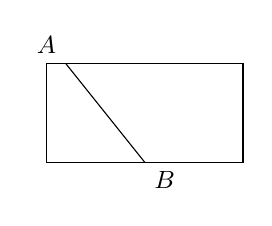
\begin{tikzpicture}[x=5mm,y=5mm,font=\small]
  \draw (0,0) rectangle (5,2.5);
  \draw (.5,2.5)node [above left] () {$A$} -- (2.5,0)node [below right] () {$B$};
\end{tikzpicture}

  \caption{}\label{fig:3.6}
 \end{minipage}\hfil
 \begin{minipage}[b]{.20\textwidth}
 \centering % (c) 2012 Dimitrios Vrettos - d.vrettos@gmail.com
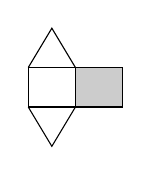
\begin{tikzpicture}[x=6mm,y=5mm]
\fill[gray, opacity=.4](1,0) rectangle (2,1);
\foreach \x in {0,1}
\draw (\x,0) rectangle  (\x+1,1);
\foreach \x in {0}
\foreach \y in {1}{
\draw (\x,\y) -- (\x+.5,\y+1)--(\x+1,\y);
\draw(\x,\y-1)--(\x+.5,-\y)--(\x+1,\y-1);}
\end{tikzpicture}

  \caption{}\label{fig:3.7}
 \end{minipage}\hfil
 \begin{minipage}[b]{.20\textwidth}
 \centering% (c) 2012 Dimitrios Vrettos - d.vrettos@gmail.com
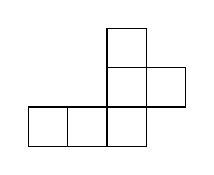
\begin{tikzpicture}[x=5mm,y=5mm]
\foreach \x in {0,1,2}
\draw (\x,0) rectangle (\x+1,1);
\foreach \y in {1,2}
\draw (2,\y) rectangle (3,\y+1);
\draw(3,1) rectangle (4,2);
\end{tikzpicture}

  \caption{}\label{fig:3.8}
 \end{minipage}\hfil
 \begin{minipage}[b]{.23\textwidth}
 \centering% (c) 2012 Dimitrios Vrettos - d.vrettos@gmail.com
\begin{tikzpicture}[x=5mm,y=5mm]
\draw (0,0) rectangle (3,3);
\end{tikzpicture}

  \caption{}\label{fig:3.9}
 \end{minipage}\hfil
\end{figure}

\begin{esercizio}
\label{ese:3.16}
Relativamente alla figura~\ref{fig:3.6}, quale proposizione è vera?

\begin{enumeratea}
\item Il segmento~$AB$ la divide in due parti uguali;
\item il segmento~$AB$ la divide in due quadrilateri.
\end{enumeratea}
\end{esercizio}

 \begin{esercizio}
 \label{ese:3.17}
La parte in grigio rappresenta~$1/4$ della figura~\ref{fig:3.7}?
\end{esercizio}

\begin{esercizio}
\label{ese:3.18}
 Costruisci una figura che sia gli~$11/6$ della figura~\ref{fig:3.8}.
\end{esercizio}

\begin{esercizio}
\label{ese:3.19}
Colora i~$3/4$ della figura~\ref{fig:3.9}.
\end{esercizio}

\begin{esercizio}
 \label{ese:3.20}
Il segmento nel disegno rappresenta i~$3/5$ dell'intero.
 \begin{center}
 % (c) 2012 Dimitrios Vrettos - d.vrettos@gmail.com
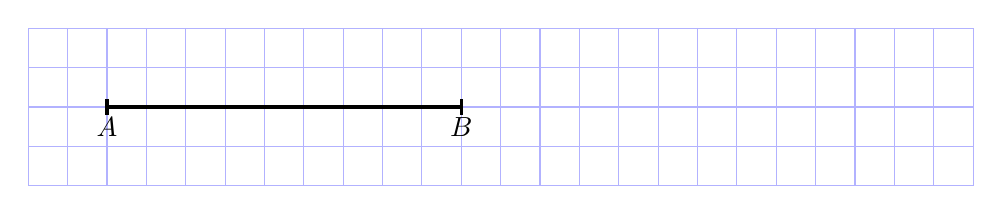
\begin{tikzpicture}
\draw[step=5mm, blue, opacity=.3](0,0) grid (120mm,20mm);
\draw[very thick](10mm,10mm) node [below] {$A$} --(55mm,10mm) node [below] {$B$};
\draw[very thick](10mm,9mm) -- (10mm,11mm);
\draw[very thick](55mm,9mm) -- (55mm,11mm);
\end{tikzpicture}

 \end{center}
Ti basta questa informazione per costruire l'intero? Come procederesti?
\end{esercizio}

\begin{esercizio}
 \label{ese:3.21}
Disegna un segmento come grandezza unitaria e dimostra che la frazione~$3/5$ è equivalente a~$6/10$ ma non a~$9/25$.
% \begin{center}
% % (c) 2012 Dimitrios Vrettos - d.vrettos@gmail.com

\begin{tikzpicture}
\draw[step=5mm, blue, opacity=.3](0,0) grid (140mm,20mm);
\end{tikzpicture}

% \end{center}
\end{esercizio}

%\begin{esercizio}eliminato da Antonio
% \label{ese:3.16}
%Usando una grandezza unitaria arbitraria, stabilisci quale delle seguenti frazioni
%rappresenta l'intero e quale un suo multiplo:
%\[\dfrac{2}{4}\text{,}\qquad\dfrac{6}{3}\text{,}\qquad\dfrac{5}{5}\text{,}\qquad\dfrac{8}{4}\text{,}\qquad
%\dfrac{9}{4}.\]
%\end{esercizio}

%%%%%%%%%%%%%%%%%%%%%%%%%%%%%%%%%%%%%%%%%%%%
%~3.3 Dalle frazioni ai numeri razionali %
%%%%%%%%%%%%%%%%%%%%%%%%%%%%%%%%%%%%%%%%%%%%
\subsubsection*{3.3 - Dalle frazioni ai numeri razionali}

%\begin{esercizio}
% \label{ese:3.17}eliminato da Antonio
%Raggruppa le seguenti frazioni in insiemi di frazioni equivalenti.
%Etichetta l'insieme con un numero razionale, prendendo per ogni gruppo la frazione ridotta ai minimi termini.
%
%\[\frac{1}{3};\,\frac{2}{4};\,-\frac{5}{2};\,\frac{6}{-14};\,\frac{-12}{4};\,\frac{3}{6};\,\frac{-3}{-9};\,
%\frac{10}{-4};\,\frac{10}{20};\,\frac{-18}{42};\,\frac{5}{15};\,-\frac{9}{21};\,-\frac{15}{6};\,\frac{4}{12}.\]
%\end{esercizio}

\begin{esercizio}
 \label{ese:3.22}
 Riscrivi le seguenti frazioni improprie come somma di un numero naturale e una frazione propria.
\[\frac{10}{3};\,\frac{17}{9};\,\frac{11}{2};\,\frac{25}{3};\,\frac{17}{10};\,\frac{15}{6}.\]
\end{esercizio}

\subsubsection*{3.4 - La scrittura dei numeri razionali}

\begin{esercizio}
 \label{ese:3.23}
 Senza eseguire le divisioni indica quali di queste frazioni possono essere scritte come numero decimale
finito (DF), quali come numero decimale periodico (DP)
e quali come numero intero (I):
 \begin{multicols}{2}
 \TabPositions{1cm}
 \begin{enumeratea}
% 	\spazielenx
 \item $-\dfrac{3}{2}$ \tab\qquad\boxDF\qquad\boxDP\quad\:\:\boxI\vspace{1.1ex}
 \item $-\dfrac{6}{5}$ \tab\qquad\boxDF\qquad\boxDP\quad\:\:\boxI\vspace{1.1ex}
 \item $\dfrac{2}{25}$ \tab\qquad\boxDF\qquad\boxDP\quad\:\:\boxI\vspace{1.1ex}
 \item $\dfrac{5}{8}$ \tab\qquad\boxDF\qquad\boxDP\quad\:\:\boxI
 \item $\dfrac{5}{6}$ \tab\qquad\boxDF\qquad\boxDP\quad\:\:\boxI\vspace{1.1ex}
 \item $-\dfrac{5}{12}$ \tab\qquad\boxDF\qquad\boxDP\quad\:\:\boxI\vspace{1.1ex}
 \item $\dfrac{12}{6}$ \tab\qquad\boxDF\qquad\boxDP\quad\:\:\boxI\vspace{1.1ex}
 \item $\dfrac{5}{10}$ \tab\qquad\boxDF\qquad\boxDP\quad\:\:\boxI
 \end{enumeratea}
 \end{multicols}
\end{esercizio}

\begin{esercizio}[\Ast]
\label{ese:3.24}
Trasforma le seguenti frazioni in numeri decimali.
\begin{multicols}{5}
\begin{enumeratea}
\spazielenx
\item $\dfrac{13}{2}$;
\item $\dfrac{11}{3}$;
\item $\dfrac{3}{5}$;
\item $\dfrac{15}{6}$;
\item $\dfrac{17}{7}$;
\item $\dfrac{15}{8}$;
\item $\dfrac{12}{9}$;
\item $\dfrac{127}{10}$;
\item $\dfrac{122}{11}$;
\item $\dfrac{13}{12}$;
\item $\dfrac{35}{121}$;
\item $\dfrac{121}{35}$;
\item $\dfrac{12}{10}$;
\item $\dfrac{127}{100}$;
\item $\dfrac{122}{\np{1100}}$;
\item $\dfrac{13}{100}$;
\item $\dfrac{35}{\np{1000}}$;
\item $\dfrac{121}{\np{10000}}$;
\item $\dfrac{12}{5}$;
\item $\dfrac{13}{7}$;
\item $\dfrac{15}{4}$;
\item $\dfrac{5}{8}$;
\item $\dfrac{32}{9}$;
\item $\dfrac{21}{20}$;
\item $\dfrac{37}{18}$;
%\item $\dfrac{2}{21}$.
\end{enumeratea}
\end{multicols}
\end{esercizio}
\pagebreak
\begin{esercizio}
\label{ese:3.25}
Trasforma le seguenti frazioni in numeri decimali.
\begin{multicols}{4}
\begin{enumeratea}
\spazielenx
\item $\dfrac{4}{12}$;
\item $\dfrac{20}{15}$;
\item $\dfrac{135}{1}$;
\item $\dfrac{28}{49}$;
\item $\dfrac{45}{9}$;
%\item $\dfrac{80}{5}$;
\item $\dfrac{8}{50}$;
\item $\dfrac{36}{1080}$;
\item $\dfrac{55}{6875}$;
\item $\dfrac{54}{648}$;
\item $\dfrac{25}{\np{0,0000002}}$;
%\item $\dfrac{28}{\np{0,00000049}}$;
\item $\dfrac{40}{\np{0,000002}}$;
\item $\dfrac{45}{\np{0,00009}}$;
\item $\dfrac{0,008}{10\times 10^{-3}}$;
\item $\dfrac{800}{5\times 10^{4}}$;
\item $\dfrac{8\times 10^{2}}{\np{50000}}$;
\item $\dfrac{12^{4}}{3^{3} \times 2^{6}}$;
\item $\dfrac{8\times 10^{-3}}{\np{0,005}}$;
\item $\dfrac{2^{3}\times \np{1000}}{500}$;
\item $\dfrac{2^{8}\times 5^{8}}{10^{8}}$;
\item $\dfrac{3^{18}}{9^{9}}$.
\end{enumeratea}
\end{multicols}
\end{esercizio}

\begin{esercizio}[\Ast]
\label{ese:3.26}
Trasforma in frazioni i seguenti numeri decimali.
\begin{multicols}{4}
\begin{enumeratea}
 \item $\np{12,5}$;
 \item $\np{4,2}$;
 \item $\np{6,25}$;
 \item $\np{3,75}$;
 \item $\np{0,1}$;
 \item $\np{2,5}$;
 \item $\np{100,100}$;
 \item $\np{0,12}$;
 \item $\np{1,1030}$;
 \item $\np{0,00100}$;
 \item $\np{100,0010}$;
 \item $\np{0,0001}$;
 \item $\np{1,25}$;
 \item $\np{0,08}$;
 \item $\np{1,002}$;
 \item $\np{15,675}$;
 \item $\np{1,7}$;
 \item $\np{1,46}$;
 \item $\np{0,13}$;
 \item $\np{0,149}$;
 \item $\np{5,015}$;
 \item $\np{3,21}$;
 \item $\np{2,3}$;
 \item $\np{1,086}$.
\end{enumeratea}
\end{multicols}
\end{esercizio}


\begin{esercizio}
 \label{ese:3.27}
Completa la tabella.

 \begin{tabular*}{.9\textwidth}{@{\extracolsep{\fill}}*{6}{lccccc}}
 \toprule
 &\multicolumn{2}{c}{Parte}& & &\\
 Numero decimale & intera & decimale & Periodo & Antiperiodo & Frazione\\
 \midrule
~$1,752\,1$& & &	& &\\
~$3,\overline{75}$& & &	& &\\
~$12,1\overline{24}$& & &	& &\\
~$1,0\overline{5}~$& & &	& &\\
~$0,13\overline{57}~$& & &	& &\\
 \bottomrule
 \end{tabular*}
\end{esercizio}

%\clearpage
\begin{esercizio}[\Ast]
\label{ese:3.28}
 Trasforma i seguenti numeri decimali in frazioni.
\begin{multicols}{4}
\begin{enumeratea}
\item $\np{-1,25}$;
\item $\np{0,03}$;
\item $\np{-2,}\overline{1}$;
\item $\np{0,}\overline{13}$;
\item $\np{5,080}$;
\item $\np{3,7}\overline{52}$;
\item $\np{-0,38}$;
\item $\np{11,}\overline{175}$;
\item $\np{0,01}\overline{0\,2}$
\item $\np{0,12}\overline{3\,45}$;
\item $\np{100,}\overline{100}$;
\item $\np{100,}\overline{001}$;
\item $\np{0,08}$;
\item $\np{0,2}$;
\item $\np{0,1}$;
\item $\np{0,03}$;
\item $\np{23,}\overline{5}$;
\item $\np{22,}\overline{32}$;
\item $\np{0,25}$;
\item $\np{31,}\overline{02}$;
\item $\np{0,}\overline{21}$;
\item $\np{2,3}\overline{4}$;
\item $\np{3,21}\overline{8}$;
\item $\np{0,03}\overline{4}$.
\end{enumeratea}
\end{multicols}
\end{esercizio}
\pagebreak
\begin{esercizio}
\label{ese:3.29}
 Scrivi delle frazioni equivalenti ai seguenti numeri decimali.
\begin{multicols}{4}
\begin{enumeratea}
\item $\np{0,00355}$;
\item $\np{3,7}$;
\item $\np{7,84}$;
\item $\np{0,004}\cdot 10^{5}$;
\item $\np{0,001}^{3}$;
\item $\np{7,42}$;
\item $\np{-0,00}\overline{6}$;
\item $\np{3}\cdot 10^{-4}$.
\end{enumeratea}
\end{multicols}
\end{esercizio}

\begin{esercizio}
\label{ese:3.30}
Scrivi la frazione generatrice di~$\np{12,3}\overline{45}$. Qual è la~614-esima cifra decimale del numero?
\end{esercizio}

\begin{esercizio}
\label{ese:3.31}
Calcola~$\np{0,}\overline{9}-\np{3,}\overline{9}$. Cosa osservi?
\end{esercizio}

\begin{esercizio}
\label{ese:3.32}
Verifica le seguenti uguaglianze trovando la frazione generatrice.
\[\frac{\np{1,}\overline{7}}{\np{1,}\overline{3}}=\np{1,}\overline{3};\qquad%
\frac{\np{2,}\overline{7}}{\np{1,}\overline{6}}=\np{1,}\overline{6};\qquad%
\frac{\np{1,}\overline{16}}{\np{2,}\overline{3}}=\np{0,5};\qquad%
\frac{\np{2,}\overline{3}}{\np{1,}\overline{6}}=\np{1,4}.\]
\end{esercizio}

\subsubsection*{3.5 - I numeri razionali e la retta}

\begin{esercizio}
 \label{ese:3.33}
Rappresenta su una retta orientata, dopo aver scelto una opportuna unità di misura,
i seguenti gruppi di numeri razionali, ciascun gruppo su una retta.
 \begin{enumeratea}
\spazielenx
 \item
 ${\displaystyle\frac{3}{4}\text{,}\quad\frac{3}{8}\text{,}\quad\frac{1}{3}\text{,}\quad\frac{5}{4}\text{,}\quad\frac{2}{5}\text{,}\quad\frac{6}{3}\text{,}\quad\frac{5}{6};\quad%
 \frac{12}{4};\quad\frac{19}{8};\quad\frac{16}{5}}$,
 \item $\displaystyle{\frac{2}{3}\text{,}\quad-\frac{3}{4}\text{,}\quad\frac{5}{2}\text{,}\quad-\frac{7}{12}\text{,}\quad\frac{3}{2}\text{,}\quad%
-\frac{11}{6}\text{,}\quad\frac{9}{4}}$;
 \item $\displaystyle{\frac{0}{4}\text{,}\quad\frac{5}{4}\text{,}\quad\frac{9}{4}\text{,}\quad\frac{1}{2}\text{,}\quad\frac{19}{8}\text{,}\quad\frac{3}{2}%
\text{,}\quad\frac{7}{4}\text{,}\quad\frac{4}{2}}$;
 \item $\displaystyle{\frac{10}{3}\text{,}\quad\frac{5}{3}\text{,}\quad~2\text{,}\quad\frac{0}{3}\text{,}\quad\frac{4}{3}\text{,}\quad\frac{2}{3}%
\text{,}\quad\frac{5}{6}\text{,}\quad\frac{13}{6}}$;
 \item $\displaystyle{\frac{1}{2}\text{,}\quad\frac{3}{4}\text{,}\quad-\frac{5}{4}\text{,}\quad-\frac{1}{2}\text{,}\quad\frac{7}{8}\text{,}%
\quad-\frac{5}{16}}$;
\item $\displaystyle{\frac{8}{5}\text{,}\quad\frac{1}{2}\text{,}\quad\frac{3}{10}\text{,}\quad-\frac{7}{4}\text{,}\quad-\frac{3}{5}%
\text{,}\quad-\frac{11}{10}}$.
 \end{enumeratea}
\end{esercizio}

\begin{esercizio}
 \label{ese:3.34}
 Scrivi i numeri razionali rappresentati dai punti segnati sulla retta nella figura.
\begin{center}
% (c) 2012 Dimitrios Vrettos - d.vrettos@gmail.com
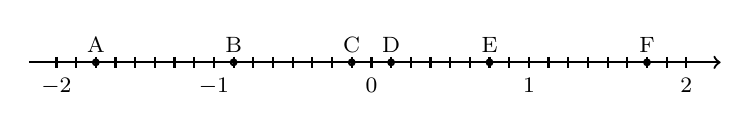
\begin{tikzpicture}
\begin{scope}[thick,font=\footnotesize]
\draw[->] (-10pt,0) -- (240pt,0);
  \foreach \x/\xtext in {%
      0/-2,.25/,.5/,.75/,
1/,1.25/,1.5/,1.75/,2/-1,2.25/,2.5/,2.75/,3/,%
      3.25/,3.5/,3.75/,4/0,4.25/,4.5/,4.75/,%
      5/,5.25/,5.5/,5.75/,6/1,6.25/,6.5/,6.75/,7/,7.25/,7.5/,7.75/,8/2}
    \draw[shift={(\x,0)}] (0pt,2pt) -- (0pt,-2pt) node[below] {$\xtext$};
\foreach \y/\ytext in {.5/$A$,2.25/$B$,3.75/$C$,4.25/$D$,5.5/$E$,7.5/$F$}
	 \draw[shift={(\y,0)}] (0pt,2pt) -- (0pt,-2pt) node[above=2pt] {$\ytext$};
\draw (.5,0) circle (1pt);
\draw (2.25,0) circle (1pt);
\draw (3.75,0) circle (1pt);
\draw (4.25,0) circle (1pt);
\draw (5.5,0) circle (1pt);
\draw (7.5,0) circle (1pt);
\end{scope}
\end{tikzpicture}

\end{center}
$ A=\ldots $,\quad $ B=\ldots $,\quad $ C=\ldots $,\quad $ D=\ldots $,\quad $ E=\ldots $,\quad $ F=\ldots $.
\end{esercizio}

\begin{esercizio}
 \label{ese:3.35}
Disegna su una retta orientata i seguenti numeri decimali, ciascun gruppo su una retta diversa.
\begin{enumeratea}
 \item $\np{0,6}$,$\qquad\np{2,3}$,$\qquad\np{-1,2}$,$\qquad\np{-0,06}$,$\qquad\np{0,3}$,$\qquad\np{0,9}$;
 \item $\np{1,4}$,$\qquad\np{-0,3}$,$\qquad\np{-1,5}$,$\qquad\np{0,2}$,$\qquad\np{-0,9}$,$\qquad\np{0,15}$;
 \item $\np{-0,8}$,$\qquad\np{-1,6}$,$\qquad\np{+4,91}$,$\qquad\np{-1,17}$,$\qquad\np{3,5}$,$\qquad\np{-2,8}$;
 \item $\np{1,55}$,$\qquad\np{2,01}$,$\qquad\np{-3,0}$,$\qquad\np{-2,10}$,$\qquad\np{0,25}$,$\qquad\np{-0,75}$.
\end{enumeratea}
\end{esercizio}
\pagebreak
\subsubsection*{3.6 - Confronto tra numeri razionali}

\begin{esercizio}
 \label{ese:3.36}
Inserisci tra le seguenti coppie di numeri razionali i simboli di maggiore~($>$), minore~($<$) o uguale~($=$).
\begin{multicols}{3}
\begin{enumeratea}
\spazielenx
 \item $\dfrac{4}{5}\,\ldots\,\dfrac{5}{7}$;
 \item $-\dfrac{9}{5}\,\ldots\,-\dfrac{8}{3}$;
 \item $-1\,\ldots\,\dfrac{1}{12}$;
 \item $\dfrac{2}{7}\,\ldots\,\dfrac{6}{21}$;
 \item $-\dfrac{1}{2}\,\ldots\,-\dfrac{3}{4}$;
 \item $\dfrac{3}{5}\,\ldots\,\dfrac{6}{9}$.
\end{enumeratea}
\end{multicols}
\end{esercizio}

\begin{esercizio}
 \label{ese:3.37}
Riscrivi in ordine crescente (dalla più piccola alla più grande) le seguenti frazioni.
\begin{enumeratea}
\item $\dfrac{2}{3}\text{,}\qquad\dfrac{3}{4}\text{,}\qquad\dfrac{5}{8}\text{,}\qquad\dfrac{3}{5}\text{,}\qquad\dfrac{7}{12}$;
\item $-\dfrac{2}{3}\text{,}\qquad-\dfrac{3}{4}\text{,}\qquad-\dfrac{5}{6}\text{,}\qquad-\dfrac{1}{2}\text{,}\qquad-\dfrac{2}{5}$;
\item $-\dfrac{2}{3}\text{,}\qquad\dfrac{3}{4}\text{,}\qquad-\dfrac{5}{6}\text{,}\qquad\dfrac{1}{2}\text{,}\qquad-1\text{,}\qquad-\dfrac{2}{5}\text{,}\qquad0.$
\item $-\dfrac{3}{2}\text{,}\qquad\dfrac{4}{3}\text{,}\qquad-\dfrac{6}{5}\text{,}\qquad\dfrac{2}{5}\text{,}\qquad-1\text{,}\qquad\dfrac{5}{2}\text{,}\qquad0$
\item $\dfrac{3}{4}\text{,}\qquad\dfrac{4}{3}\text{,}\qquad\dfrac{11}{12}\text{,}\qquad\dfrac{5}{3}\text{,}\qquad\dfrac{2}{3}\text{,}\qquad\dfrac{2}{7}\text{,}\qquad\dfrac{3}{2}$.
\end{enumeratea}
\end{esercizio}

\begin{esercizio}
 \label{ese:3.38}
Ordina dal più piccolo al più grande i seguenti valori.
\begin{enumeratea}
\item $\np{10,011}$,$\qquad\np{10,110}$,$\qquad\np{11,001}$,$\qquad\np{11,100}$;
\item $\np{10,01}$,$\qquad\np{11,11}$,$\qquad\np{10,101}$,$\qquad\np{10,001}$;
\item $\np{0,101}$,$\qquad\np{0,011}$,$\qquad\np{0,110}$,$\qquad\np{0,0101}$;
\item $\np{1,0101}$,$\qquad\np{1,1001}$,$\qquad\np{1,0011}$,$\qquad\np{1,0110}$.
\end{enumeratea}
\end{esercizio}

\begin{esercizio}
\label{ese:3.39}
Scrivi una frazione molto vicina a~$-\dfrac{2}{9}.$
\end{esercizio}

\begin{esercizio}
\label{ese:3.40}
Scrivi una frazione compresa tra:
\begin{multicols}{3}
\begin{enumeratea}
\item $\dfrac{3}{5}$ e~$\dfrac{7}{10}$;
\item $\dfrac{5}{3}$ e~$\dfrac{1}{7}$;
\item $\dfrac{1}{2}$ e~$\dfrac{2}{3}$.
\end{enumeratea}
\end{multicols}
\end{esercizio}

\begin{esercizio}
\label{ese:3.41}
Quali disuguaglianze sono vere?
\begin{multicols}{2}
\TabPositions{2.5cm}
\begin{enumeratea}
\spazielenx
 \item $-\dfrac{7}{6}<-\dfrac{6}{7}$;\tab\boxV\qquad\boxF
 \item $-\dfrac{7}{6}>+\dfrac{6}{7}$;\tab\boxV\qquad\boxF
 \item $-\dfrac{7}{6}<+\dfrac{6}{7}$;\tab\boxV\qquad\boxF
 \item $+\dfrac{7}{6}<-\dfrac{6}{7}$;\tab\boxV\qquad\boxF
 \item $+\dfrac{7}{6}<+\dfrac{6}{7}$;\tab\boxV\qquad\boxF
 \item $+\dfrac{7}{6}>-\dfrac{6}{7}$.\tab\boxV\qquad\boxF
 \end{enumeratea}
\end{multicols}
\end{esercizio}

\begin{esercizio}
\label{ese:3.42}
Quale dei seguenti numeri è più vicino a~1?
\[\boxA\quad\np{0,10}\qquad\boxB\quad\np{0,99}\qquad\boxC\quad\np{0,01}\qquad\boxD\quad\np{0,90}\]
\end{esercizio}

 \begin{esercizio}
\label{ese:3.43}
Quale dei seguenti numeri è più vicino alla frazione~$\dfrac{1}{10}$?
\[\boxA\quad\np{0,01}\qquad\boxB\quad\np{0,90}\qquad\boxC\quad\np{1,01}\qquad\boxD\quad\np{0,19}\]
 \end{esercizio}
\pagebreak
\begin{esercizio}
\label{ese:3.44}
Scrivi due numeri compresi tra:
\begin{multicols}{3}
\begin{enumeratea}
 \item $\np{2,3}$ e $\np{3,4}$;
 \item $\np{3,4}$ e $\np{3,6}$;
 \item $\np{2,}\overline{3}$ e~$\np{2,}\overline{4}$;
 \item $\np{1,1}\overline{3}$ e~$\np{1,2}\overline{3}$;
 \item $\np{3,}\overline{4}$ e~$\np{3,}\overline{6}$;
 \item $\np{1,}\overline{35}$ e~$\np{1,}\overline{36}$.
\end{enumeratea}
\end{multicols}
\end{esercizio}

%\begin{esercizio}
% \label{ese:3.43}
%Rappresenta su una opportuna retta numerica le seguenti frazioni e poi riscrivile in ordine
%crescente:
%\[\frac{3}{4}\text{,~~}\frac{3}{8}\text{,~~}\frac{1}{3}\text{,~~}\frac{5}{4}\text{,~~}\frac{2}{5}\text{,~~}\frac{6}{3}\text{,~~}\frac{5}{6}\text{,~~}\frac{12}{4}\text{,~~}\frac{19}{8}\text{,~~}\frac{16}{5}.\]
%\end{esercizio}

%%%%%%%%%%%%%%%%%%%%%%%%%%%%%%%%%%%%%%%%%%%%%%%%%%%%%%%%%%%
\subsubsection*{3.7 - Le operazioni con i numeri razionali}


\begin{esercizio}[\Ast]
 \label{ese:3.45}
Calcola le seguenti somme algebriche tra frazioni.
\begin{multicols}{4}
\begin{enumeratea}
\spazielenx
\item $\dfrac{1}{2} + \dfrac{3}{2}$;
\item $\dfrac{7}{11} + \dfrac{4}{11}$;
\item $\dfrac{3}{2} - \dfrac{5}{2}$;
\item $\dfrac{8}{18} + \dfrac{5}{9}$;
\item $\dfrac{6}{5} + 0$;
\item $-\dfrac{3}{2}+\dfrac{4}{3}$;
\item $-\dfrac{2}{3}+\dfrac{3}{4}$;
\item $\dfrac{4}{3}-\dfrac{6}{5}$;
\item $\dfrac{2}{5}+\dfrac{5}{8}$;
\item $\dfrac{5}{8}+\dfrac{5}{6}$;
\item $\dfrac{5}{6}-\dfrac{5}{12}$;
\item $1-\dfrac{3}{2}$;
\item $\dfrac{11}{5}+5$;
\item $\dfrac{7}{3}-\dfrac{6}{4}$;
\item $3-\dfrac{2}{3}$;
\item $\dfrac{1}{5}-1$;
\item $4+\dfrac{3}{2}-\dfrac{3}{4}$;
\item $\dfrac{4}{3}+3-\dfrac{1}{2}$;
\item $\dfrac{3}{4}+\dfrac{1}{4}-\dfrac{5}{4}$;
\item $1-\dfrac{1}{2}+\dfrac{1}{3}-\dfrac{1}{4}$.
\end{enumeratea}
\end{multicols}
\end{esercizio}

\begin{esercizio}
 \label{ese:3.46}
Calcola le seguenti somme algebriche fra numeri razionali.
\begin{multicols}{3}
\begin{enumeratea}
\spazielenx
\item $\np{1,}\overline{6}+\dfrac{2}{3}$;
\item $\np{5,1}-\np{1,}\overline{5}$;
\item $\np{0,03}+\dfrac{0}{3}$;
\item $\np{0,1}\overline{6}-\np{1,}\overline{45}$;
\item $50\%+\dfrac{1}{2}$;
\item $\dfrac{2}{5}-\np{1,2}+5\%$;
\item $\np{-1,}\overline{2}+25\%+\dfrac{5}{18}$;
\item $\dfrac{3}{2}-13\%+\np{0,15}$;
\item $\np{1,}\overline{2}+\np{1,2}+\dfrac{1}{2}+\np{1,2}\%~$;
\item $\np{7,9892}+\np{3,1218}$;
\item $\np{3,999}+ \text{un centesimo}$.
\end{enumeratea}
\end{multicols}
\end{esercizio}

\begin{esercizio}
Completa:
 \label{ese:3.47}
\[\frac{3}{4}+\ldots=1;\qquad1-\ldots=\frac{4}{13};\qquad\frac{11}{12}\cdot\ldots=\frac{8}{55};%
\qquad\ldots:\frac{5}{3}=\frac{3}{5}.\]
\end{esercizio}

\begin{esercizio}
 \label{ese:3.48}
Completa la seguente tabella.

 \begin{tabular*}{.9\textwidth}{@{\extracolsep{\fill}}*{8}{c}}
 \toprule
~$a$ &~$-\dfrac{2}{3}$ &~$+\dfrac{3}{4}$ &~$-1$ &~0 &~$\np{-1,}\overline{6}$ &$-5$ &$\np{-0,21}$\vspace{1.05ex}\\
~$b$ &~$+\dfrac{7}{3}$ &~$-\dfrac{5}{8}$ &~$+\dfrac{2}{5}$ &~15\% &%
~$\np{+2,}\overline{3}$ &$+\dfrac{17}{3}$ &$+\dfrac{3}{5}$\\
\midrule
~$a+b$& & &	& & & &\\
~$a-b$& & &	& & & &\\
~$b-a$& & &	& & & &\\
~$-a-b$& & &	& & & &\\
~$-a+b$& & &	& & & &\\
 \bottomrule
 \end{tabular*}
\end{esercizio}
\pagebreak
\begin{esercizio}
 \label{ese:3.49}
Completa la seguente tabella.
\begin{center}
 % (c) 2012 Dimitrios Vrettos - d.vrettos@gmail.com
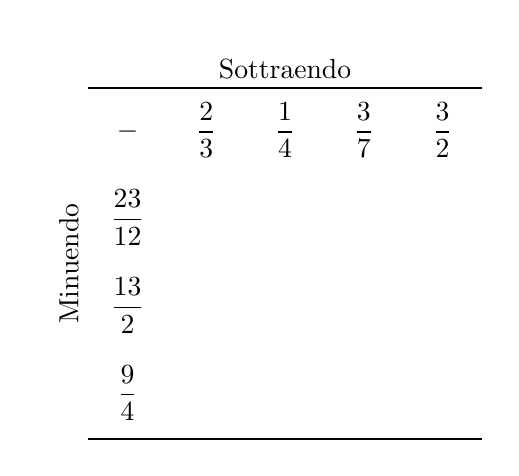
\begin{tikzpicture}[x=8mm, y=8mm, every node/.style={anchor=base,text height=1.5em,text depth=1em,minimum size=10mm}]

\matrix (a) [matrix of nodes]{
$-$ &$\displaystyle{\frac{2}{3}}$ &$\displaystyle{\frac{1}{4}}$ &$\displaystyle{\frac{3}{7}}$ &$\displaystyle{\frac{3}{2}}$\\
$\displaystyle\frac{23}{12}$ & & & &\\
$\displaystyle\frac{13}{2}$ & & & &\\
$\displaystyle\frac{9}{4}$ & & & &{}\\
};

\node[] at (a.north) {Sottraendo};
\node[rotate=90] at (a.west) {Minuendo};
\draw[thick] (a-1-1.north west)--(a-1-5.north east);
\draw[thick] (a-4-1.south west)--(a-4-5.south east);
\end{tikzpicture}

\end{center}
\end{esercizio}

\begin{esercizio}
 \label{ese:3.50}
Calcola a mente:
\begin{multicols}{3}
\begin{enumeratea}
\item $\np{0,1}+\np{0,1}$;
\item $\np{0,2}+\np{0,8}$;
\item $\np{0,01}+\np{0,9}$
\item $\np{0,91}+\np{0,19}$;
\item $\np{1,10}+\np{1,01}$;
\item $\np{0,999}+\np{0,10}$;
\item $\np{1,1}-\np{0,9}$;
\item $\np{100}-\np{0,99}$;
\item $2-\np{0,1}$;
\item $3-\np{1,1}$;
\item $4-\np{1,4}$;
\item $10-\np{0,10}$.
\end{enumeratea}
\end{multicols}
\end{esercizio}

%%%%%%%%%%%%%%%%%%%%%%%%%%%%%%%%%
% Moltiplicazione

\begin{esercizio}
 \label{ese:3.51}
Calcola i seguenti prodotti fra frazioni.
\begin{multicols}{3}
\begin{enumeratea}
\spazielenx
 \item $\dfrac{3}{2}\cdot\dfrac{4}{3}$;
 \item $6\cdot\dfrac{5}{2}$;
 \item $-\dfrac{6}{5}\cdot\Bigg(-\dfrac{4}{3}\Bigg)$;
 \item $\dfrac{2}{3}\cdot\dfrac{2}{9}$;
 \item $\dfrac{5}{5}\cdot\dfrac{5}{8}\cdot\Bigg(-\dfrac{5}{6}\Bigg)$;
 \item $\dfrac{3}{2}\cdot\Bigg(-\dfrac{8}{9}\Bigg)\cdot\dfrac{5}{6}$;
\end{enumeratea}
\end{multicols}
\end{esercizio}

\begin{esercizio}
 \label{ese:3.52}
Calcola i seguenti prodotti fra numeri razionali.
\[\np{-1,}\overline{1}\cdot\frac{18}{5};\qquad2\%\cdot5\%;\qquad-\frac{3}{4}\cdot(-120\%).\]
\end{esercizio}

\begin{esercizio}
 \label{ese:3.53}
Completa la seguente tabella.

 \begin{tabular*}{.9\textwidth}{@{\extracolsep{\fill}}*{8}{c}}
 \toprule
~$a$ &~$-\dfrac{2}{3}$ &~$+\dfrac{3}{4}$ &~$-\dfrac{5}{8}$ &~15\% %
&~$\np{-1,}\overline{6}$ &$+\dfrac{17}{3}$ &$\np{-0,21}$\vspace{1.05ex}\\
~$b$ &~$+\dfrac{7}{3}$ & &~$-\dfrac{5}{2}$ & &%
~$\np{+2,}\overline{3}$ & &$+\dfrac{5}{3}$\\
\midrule
~$a\cdot b$& &~1 &	&$-1$ & &0 &\\
 \bottomrule
 \end{tabular*}
\end{esercizio}
\pagebreak
\begin{esercizio}
 \label{ese:3.54}
 Completa la seguente tabella.
\begin{center}
 % (c) 2012 Dimitrios Vrettos - d.vrettos@gmail.com
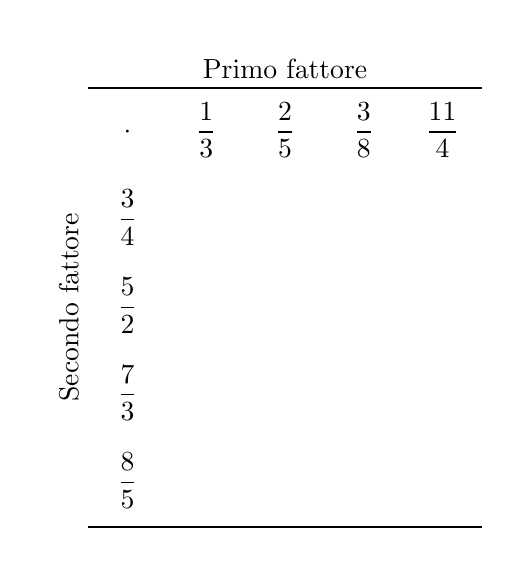
\begin{tikzpicture}[x=8mm, y=8mm, every node/.style={anchor=base,
    text height=1.5em,text depth=1em,minimum size=10mm}]

\matrix (a) [matrix of nodes]{
$\cdot$ &$\displaystyle{\frac{1}{3}}$ &$\displaystyle{\frac{2}{5}}$ &$\displaystyle{\frac{3}{8}}$ &$\displaystyle{\frac{11}{4}}$\\
$\displaystyle\frac{3}{4}$ & & & &\\
$\displaystyle\frac{5}{2}$ & & & &\\
$\displaystyle\frac{7}{3}$ & & & &{}\\
$\displaystyle\frac{8}{5}$ & & & &{}\\
};

\node[] at (a.north) {Primo fattore};
\node[rotate=90] at (a.west) {Secondo fattore};
\draw[thick] (a-1-1.north west)--(a-1-5.north east);
\draw[thick] (a-5-1.south west)--(a-5-5.south east);
\end{tikzpicture}
\end{center}
\end{esercizio}

\begin{esercizio}
 \label{ese:3.55}
Calcola a mente:
\begin{multicols}{4}
 \begin{enumeratea}
 \spazielenx
\item $\np{0,1}\cdot \np{0,1}$;
\item $\dfrac{1}{10}\cdot\dfrac{1}{10}$;
\item $\np{0,1}\cdot 100$;
\item $1\cdot \np{0,1}$;
\item $2\cdot \np{0,1}$;
\item $20\cdot \np{0,02}$;
\item $\np{0,01}\cdot 10$;
\item $\dfrac{1}{100}\cdot 10$;
\item $\np{0,1}\cdot \np{0,2}$;
\item $\dfrac{3}{10}\cdot 30$;
\item $\np{0,01}\cdot \np{0,1}$;
\item $\np{1000}\cdot \np{0,0001}$.
 \end{enumeratea}
\end{multicols}
\end{esercizio}

%%%%%%%%%%%%%%%%%%%%%%%%%%%%%%%%%%%%%%
% Divisione

\begin{esercizio}
 \label{ese:3.56}
Calcola i seguenti quozienti fra frazioni.
\begin{multicols}{4}
\begin{enumeratea}
\item $\dfrac{3}{2}:\dfrac{4}{3}$;
\item $-\dfrac{6}{5}:\bigg(-\dfrac{2}{3}\bigg)$;
\item $\dfrac{+3}{2}:\bigg(\dfrac{-3}{2}\bigg)$;
\item $\dfrac{2}{5}:\dfrac{5}{8}:\bigg(-\dfrac{5}{6}\bigg)$.
\end{enumeratea}
\end{multicols}
\end{esercizio}

\begin{esercizio}
 \label{ese:3.57}
Calcola i seguenti quozienti fra numeri razionali.
\begin{multicols}{2}
\begin{enumeratea}
\spazielenx
\item $\np{-1,}\overline{1}:\dfrac{18}{5}$;
\item $2\%:5\%$;
\item $\dfrac{1}{2}:0,5$;
\item $-\dfrac{3}{4}:\np{1,4}:(-120\%)$.
\end{enumeratea}
\end{multicols}
\end{esercizio}

\pagebreak

\begin{esercizio}
 \label{ese:3.58}
Completa la seguente tabella.

 \begin{tabular*}{.9\textwidth}{@{\extracolsep{\fill}}*{8}{c}}
 \toprule
~$a$ &~$-\dfrac{2}{3}$ &~$+\dfrac{3}{4}$ &~$-1$ &~0 %
&~$\np{-1,}\overline{6}$ &$-5$ &$\np{-0,21}$\vspace{1.05ex}\\
~$b$ &~$+\dfrac{7}{3}$ &~$-\dfrac{5}{8}$ &~$+\dfrac{2}{5}$ &~15\%&%
~$\np{+2,}\overline{3}$ &$+\dfrac{17}{3}$ &~$+\dfrac{3}{5}$\\
\midrule
~$a:b$& & &	& & & &\\
~$b:a$& & &	& & & &\\
\bottomrule
 \end{tabular*}
\end{esercizio}

\begin{esercizio}
 \label{ese:3.59}
Calcola a mente:
\begin{multicols}{4}
 \begin{enumeratea}
 \spazielenx
\item $\np{0,30}\cdot\np{0,40}$;
\item $\np{0,5}:\np{0,1}$;
\item $\np{0,5}\cdot\np{0,2}$;
\item $\np{0,1}\cdot\np{0,1}$;
\item $\np{0,4}\cdot 3$;
\item $\np{0,1}:\np{0,1}$;
\item $\np{0,5}\cdot 20$;
\item $\np{0,1}\cdot\np{0,010}$.
 \end{enumeratea}
\end{multicols}
\end{esercizio}

\begin{esercizio}
 \label{ese:3.60}
Esegui le seguenti operazioni con le frazioni, quando è possibile.
\begin{multicols}{3}
\begin{enumeratea}
\spazielenx
\item $\displaystyle{\frac{2}{3}\cdot0}$;
\item $\displaystyle{\frac{1}{2}-\frac{1}{2}}$;
\item $\displaystyle{\frac{1}{2}\cdot\frac{2}{0}}$;
\item $\displaystyle{\frac{1}{2}}\cdot\frac{0}{2}$;
\item $\displaystyle{\frac{1}{2}\cdot\frac{1}{2}}$;
\item $\displaystyle{\frac{2}{3}:0}$;
\item $\displaystyle{\frac{2}{3}-0}$;
\item $\displaystyle{1:\frac{2}{3}}$;
\item $\displaystyle{\frac{1}{4}\cdot4}$;
\item $\displaystyle{\frac{1}{4}:4}$;
\item $\np{0,3}:3$;
\item $\displaystyle{\np{1,5}:\np{1,}\overline{5}}$;
\item $\np{1,5}:\np{1,5}$;
\item $\np{1,5}^0$;
\item $(1-1)^0$;
\item $(-1)^{-1}$;
\item $3^0:2^0$;
\item $(-2)^{-2}:(-1)^{-1}$.
\end{enumeratea}
\end{multicols}
\end{esercizio}

\subsubsection*{3.8 - Potenza di una frazione}

\begin{esercizio}
 \label{ese:3.61}
Calcola il valore delle seguenti potenze.
\begin{multicols}{4}
\begin{enumeratea}
\spazielenx
 \item $\bigg(-\dfrac{2}{3}\bigg)^2$;
 \item $\bigg(-\dfrac{1}{2}\bigg)^3$;
 \item $\bigg(-\dfrac{3}{2}\bigg)^2$;
 \item $\bigg(\dfrac{1}{2}-1\bigg)^3$;
 \item $\bigg(-\dfrac{3}{5}\bigg)^0$;
 \item $\bigg(-\dfrac{3}{5}\bigg)^1$;
 \item $-2^4$;
 \item $(-2)^4$;
 \item $\bigg(-\dfrac{2}{3}\bigg)^{-2}$;
 \item $\bigg(-\dfrac{1}{2}\bigg)^{-3}$;
 \item $-\bigg(\dfrac{3}{2}\bigg)^{-2}$;
 \item $-2^{-4}$;
 \item $(-2)^{-4}$;
 \item $-\bigg(\dfrac{5}{6}\bigg)^{-1}$.
\end{enumeratea}
\end{multicols}
\end{esercizio}

\begin{esercizio}
 \label{ese:3.62}
Indica quali proprietà delle potenze sono state applicate nelle seguenti uguaglianze.
\begin{enumeratea}
\spazielenx
 \item $\displaystyle{\bigg(-\frac{3}{2}\bigg)^2\cdot\bigg(-\frac{3}{2}\bigg)^{3}=%
\bigg(-\frac{3}{2}\bigg)^{5}=-\frac{3^5}{2^5}}$;\quad proprietà \dotfill
 \item $\displaystyle{\bigg(-\frac{3}{2}\bigg)^2:\bigg(-\frac{3}{2}\bigg)^{3}=\bigg(-\frac{3}{2}\bigg)^{-1}=%
-\frac{2}{3}}$;\quad proprietà \dotfill
 \item $\displaystyle{\Bigg(\bigg(-\frac{3}{2}\bigg)^2\Bigg)^3=\bigg(-\frac{3}{2}\bigg)^{6}=%
+\frac{3^6}{2^6}}$;\quad proprietà \dotfill
 \item $\displaystyle{\bigg(\frac{5}{2}\bigg)^2:\bigg(\frac{25}{10}\bigg)^2=\bigg(\frac{5}{2}:\frac{5}{2}\bigg)^2=%
\bigg(\frac{5}{2}\cdot\frac{2}{5}\bigg)^2=1^2}$;\quad proprietà \dotfill
 \item $\displaystyle{\bigg(-\frac{5}{2}\bigg)^{2}\cdot\bigg(\frac{6}{25}\bigg)^{2}=\bigg(-\frac{5}{2}\cdot%
\frac{6}{25}\bigg)^{2}=\bigg(-\frac{3}{5}\bigg)^2=+\frac{3^2}{5^2}}$;\quad proprietà \dotfill
\end{enumeratea}
\end{esercizio}

\begin{esercizio}
 \label{ese:3.63}
Completa la seguente tabella.

 \begin{tabular*}{.9\textwidth}{@{\extracolsep{\fill}}*{8}{c}}
 \toprule
~$a$ &~$a^2$ &~$a^{-2}$ &~$-a^2$ &~$(-a)^3$ &~$a^{-1}$ &~$a^0$ &$a^3$\\
\midrule
~$\displaystyle{-\frac{2}{3}}$& & &	& & & &\vspace{1.05ex}\\
~$\np{-1,}\overline{6}$& & &	& & & &\\
 $\np{-0,1}$& & &	& & & &\\
~$\dfrac{3}{10}$& & &	& & & &\vspace{1.05ex}\\
\bottomrule
 \end{tabular*}
\end{esercizio}

\begin{esercizio}
 \label{ese:3.64}
Calcola a mente.
\begin{multicols}{4}
\begin{enumeratea}
 \item $\np{3,4}\cdot10^2$;
 \item $\np{3,4}:10^2$;
 \item $\np{0,34}\cdot10^4$;
 \item $\np{34,4}:10^2$;
 \item $\np{0,34}\cdot10^3$;
 \item $\np{34,10}\cdot10^3$;
 \item $\np{3,04}\cdot10$;
 \item $\np{0,34}:10^2$.
\end{enumeratea}
\end{multicols}
\end{esercizio}

\begin{esercizio}
 \label{ese:3.65}
Calcola le seguenti potenze prestando particolare attenzione ai segni.
\begin{multicols}{3}
\begin{enumeratea}
 \spazielenx
 \item $-(-2)^2$;
 \item $[-(-1)^{2}]^3$;
 \item $-(-2)^{-4}$;
 \item $-[-(-1)^{-1}]^{-2}$;
 \item $\dfrac{2^{-1}+3^{-2}}{2^{-2}+3^{-1}}$;
 \item $\dfrac{2^{-2}-3^{-1}}{2^{-2}+3^{-1}}$;
 \item $(-3)^3\cdot\dfrac{2^{-2}-5^{-1}}{2^{-2}+5^2}$.
\end{enumeratea}
\end{multicols}
\end{esercizio}

\subsubsection*{3.10 - Notazione scientifica e ordine di grandezza}

\begin{esercizio}
 \label{ese:3.66}
Esprimere in notazione scientifica i seguenti numeri.
\begin{multicols}{2}
\begin{enumeratea}
\item $\np{780000000000000}=\np{7,8}\cdot10^{\ldots}$;
\item $\np{423000000000}=\np{4,23}\cdot10^{\ldots}$;
\item $\np{76000000000000}= \ldots \cdot 10^{\ldots}$;
\item $\np{0,00000000098}=\np{9,8}\cdot10^{\ldots}$;
\item $\np{0,0000045}=\np{4,5}\cdot10^{\ldots}$;
\item $\np{0,000000987}= \ldots \cdot 10^{\ldots}$.
\end{enumeratea}
\end{multicols}
\end{esercizio}

\begin{esercizio}
 \label{ese:3.67}
Quale tra i seguenti numeri non è scritto in notazione scientifica?

\boxA\quad$\np{5,67e-12}$\qquad
\boxB\quad$\np{4,28e8}$\qquad
\boxC\quad$\np{10,3e-2}$\qquad
\boxD\quad$\np{9,8e7}$\qquad
\end{esercizio}

\begin{esercizio}
 \label{ese:3.68}
Determina in notazione scientifica l'area di una lamina di ferro quadrata
avente il lato di misura~$\np[m]{0,00000000021}$.
\end{esercizio}

\begin{esercizio}
 \label{ese:3.69}
Scrivi in notazione scientifica i seguenti numeri.
\[\np{34000};\qquad\np{0,000054};\qquad\np{26};\qquad\np{0,54000};\qquad\np{5};\qquad\np{0,00001};\qquad\np{990000};\qquad\np{222}.\]
\end{esercizio}
\pagebreak
\begin{esercizio}
 \label{ese:3.70}
Trasforma i numeri in notazione scientifica e scrivi nella stessa forma il risultato.
\begin{multicols}{2}
\begin{enumeratea}
\item $\np{0,00036}\cdot\np{20000000}=\ldots$;
\item $\np{8400}:42=\ldots$;
\item $\np{900000000}:\np{0,0003}=\ldots$;
\item $3:\np{10000000}=\ldots$
\end{enumeratea}
\end{multicols}
\end{esercizio}

\begin{esercizio}
 \label{ese:3.71}
Calcola ed esprimi il risultato in notazione scientifica.
\begin{multicols}{2}
\begin{enumeratea}
\item $\np{3e24}+\np{4e24}$;
\item $\np{0,3e104}+\np{4e103}$;
\item $\np{6e101}\cdot\np{0,15e101}$;
\item $\np{12e2000}:\np{6e200}$.
\end{enumeratea}
\end{multicols}
\end{esercizio}

\begin{esercizio}[\Ast]
 \label{ese:3.72}
Trasforma i numeri in notazione scientifica e scrivi nella stessa forma il risultato.
\begin{multicols}{2}
\begin{enumeratea}
\item $\dfrac{(\np{0,00002})^2:\np{30000000} \cdot (\np{0,1})^5}{\np{4000} \cdot \np{0,02}:\np{0,000003}}$;\vspace{1.1ex}
\item $\dfrac{\np{95000000}\cdot\np{0,000072}}{(\np{250000})^{3} :(\np{0,000035})^{2}}$;\vspace{1.1ex}
\item $\dfrac{(\np{3000})^2:\np{0,000003}:\np{20000000}}{\np{0,00002}:\np{0,00000004}}$;
\item $\dfrac{(6,3\cdot10^{6})^{2}\cdot \np{0,0000031}}{(\np{40000000})^4 : (8\cdot 10^{-18})^{4}}$;\vspace{1.1ex}
\item $\dfrac{(\np{2000})^3 \cdot (\np{0,000001})^5:20}{(\np{0,0003})^2:\np{3000000}}$;\vspace{1.1ex}
\item $\dfrac{\np{4000}^2\cdot \np{0,000012}}{\np{3e9}\cdot \np{2000}^3}$.
\end{enumeratea}
\end{multicols}
\end{esercizio}

\begin{esercizio}
 \label{ese:3.73}
Disponi in ordine di distanza dal Sole i seguenti pianeti, in base alla distanza media in km riportata
tra parentesi: Mercurio~($\np{5,8e7}$), Nettuno~($\np{4,5e9}$), Giove~($\np{7,8e8}$),
Plutone~($\np{6,1e9}$), Urano~($\np{2,7e9}$), Terra~($\np{1,5e8}$), Marte~($\np{2,3e8}$).
\end{esercizio}

%%%%%%%%%%%%%%%%%%%%%%%%%%%%%%%%%%
% Ordine di grandezza

\begin{esercizio}
 \label{ese:3.74}
Determina l'ordine di grandezza dei seguenti numeri.
\begin{multicols}{4}
\begin{enumeratea}
\item $\np{126000000}$;
\item $\np{0,0000098}$;
\item $\np{7000000}$;
\item $\np{0,0000000027}$.
\end{enumeratea}
\end{multicols}
\end{esercizio}

\begin{esercizio}
 \label{ese:3.75}
Completa la seguente tabella.

 \begin{tabular*}{.9\textwidth}{@{\extracolsep{\fill}}*{5}{c}}
 \toprule
 Numero &~$\np{26000000}$ &~$\np{0,000083}$ &~$\np{490000}$ &~$\np{0,0000081}$\\
\midrule
 Notazione scientifica& & &	&\\
 o.d.g.& & &	&\\
\bottomrule
 \end{tabular*}
\end{esercizio}

\begin{esercizio}
 \label{ese:3.76}
Determina l'ordine di grandezza del risultato dei seguenti calcoli.
\begin{multicols}{2}
\begin{enumeratea}
\item $\np{5,3e5}\cdot\np{1,2e3}-\np{2,5e6}$;
\item $(\np{5e2}\cdot\np{4e3})^3$.
\end{enumeratea}
\end{multicols}
\end{esercizio}

\subsubsection*{3.11 - Problemi con le frazioni}

\begin{esercizio}[\Ast]
 \label{ese:3.77}
La distanza Roma - Bari è di~$450\unit{km}$. Se ho percorso i~$2/5$ del tragitto quanti chilometri
mancano ancora da percorrere?
\end{esercizio}

\begin{esercizio}[\Ast]
 \label{ese:3.78}
Lucia ha letto~$3/5$ di un libro e le rimangono da leggere~$120$ pagine. Di quante pagine è composto il libro?
\end{esercizio}

\begin{esercizio}[\Ast]
 \label{ese:3.79}
Una persona possiede \officialeuro~$525$. Se spende i~$3/5$ della somma e poi i~$2/3$ della rimanente,
quale somma di denaro le rimane?
\end{esercizio}

\begin{esercizio}
 \label{ese:3.80}
Luigi ha~$18$ anni, cioè i~$3/7$ dell'età di sua madre, che a sua volta ha i~$4/5$ dell'età
del padre. Quali sono le età del padre e della madre di Luigi?
\end{esercizio}

\subsubsection*{3.12 - Le percentuali}

\begin{esercizio}
 \label{ese:3.81}
Trasforma i seguenti numeri percentuali in numeri decimali.
\[12\%;\quad \np{0,03}\%;\quad \np{4,3}\%;\quad 80\%;\quad \np{3,5}\%;\quad\np{-0,2}\%;\quad 15\%;\quad\np{-0,38}\%.\]
\end{esercizio}

\begin{esercizio}
 \label{ese:3.82}
Trasforma i seguenti numeri decimali in percentuali.
\[\np{-1,25};\quad \np{0,03};\quad \np{-2,}\overline{1};\quad \np{0,}\overline{13};\quad \np{5,080};\quad \np{3,7}\overline{52};\quad \np{-0,38}.\]
\end{esercizio}

\begin{esercizio}
 \label{ese:3.83}
Trasforma i seguenti numeri percentuali in frazioni ridotte ai minimi termini.
\[12\%;\quad \np{0,03}\%;\quad \np{4,3}\%;\quad 80\%;\quad \np{3,5}\%;\quad \np{-0,2}\%;\quad 15\%;\quad\np{-0,38}\%.\]
\end{esercizio}

\begin{esercizio}
\label{ese:3.84}
Trasforma le seguenti frazioni in numeri percentuali.
\[-\frac{3}{2};\quad\frac{4}{3};\quad-\frac{6}{5};\quad\frac{2}{25};\quad\frac{5}{8};
\quad\frac{5}{6};\quad-\frac{5}{12}.\]
\end{esercizio}

% Problemi con gli sconti
\begin{esercizio}
 \label{ese:3.85}
A una scuola di ballo si sono iscritte~$120$ persone delle quali il~$20\%$ frequenta i corsi di ballo liscio.
In quanti frequentano i corsi di liscio?
\end{esercizio}

\begin{esercizio}
 \label{ese:3.86}
Una scuola attiva dei corsi di lingue. $32$~studenti si iscrivono al corso di inglese, 24 al
corso di francese e 16 al corso di tedesco.
Qual è la percentuale degli alunni iscritti al corso di inglese, rispetto al totale degli iscritti?
\end{esercizio}

\begin{esercizio}
 \label{ese:3.87}
A una scuola di ballo sono iscritte~$120$ persone e di queste il~$68\%$ sono donne. Quanti sono gli uomini?
\end{esercizio}

\begin{esercizio}
 \label{ese:3.88}
 Il prezzo di listino di una bici è di \officialeuro~$175$. Se viene venduta con uno sconto del~$10\%$ quanto viene a costare?
\end{esercizio}

\begin{esercizio}[\Ast]
 \label{ese:3.89}
Una canna da pesca da \officialeuro~$125$ è in vendita promozionale a \officialeuro~$70$.
Qual è la percentuale di sconto applicata?
\end{esercizio}

\begin{esercizio}[\Ast]
 \label{ese:3.90}
Per l'acquisto di un armadio, Maria è riuscita a spuntare, dopo lunghe discussioni con il venditore, uno sconto del~$25\%$, risparmiando ben \officialeuro~$120$. Qual era il prezzo dell'armadio prima dello sconto?
\end{esercizio}

\begin{esercizio}
\label{ese:3.91}
Completa la seguente tabella.

\begin{tabular*}{.9\textwidth}{@{\extracolsep{\fill}}*{4}{c}}
\toprule
Prezzo di listino (\officialeuro)&	Sconto (\officialeuro)& sconto ($\%$)	&Prezzo scontato (\officialeuro)\\
\midrule
120 & 12 & 10 & 108\\
250&10&&\\
125&5&&\\
170&&10&\\
\np{1100}&&15&\\
220&&&20\\ 	
\np{12000}&&&700\\
&15&15&\\
&30&&50\\
&&25&140\\	
&120&30&\\
\bottomrule
\end{tabular*}
\end{esercizio}
\pagebreak
\begin{esercizio}
\label{ese:3.92}
Calcola:
\begin{multicols}{3}
\begin{enumeratea}
\item il~$10\%$ di~$100$;
\item il~$30\%$ di~$700$;
\item il~$20\%$ di~$500$;
\item il~$15\%$ di~$150$;
\item il~$25\%$ di~$\np{1250}$;
\item il~$16\%$ di~$120$.
\end{enumeratea}
\end{multicols}
\end{esercizio}

\begin{esercizio}
 \label{ese:3.93}
Quale percentuale è:
\begin{enumeratea}
 \item $10$ bocciati su~$120$ alunni: la percentuale di bocciati è circa $8,3\%$;
 \item $15$ alunni su~$45$ giocano a calcio: la percentuale di alunni che giocano a calcio è \ldots\ldots;
 \item $10$ alunni su~$28$ suonano il piano: la percentuale di alunni che suonano il piano è \ldots\ldots;
 \item $20$ alunni su~$120$ frequentano il corso di teatro: la percentuale di alunni che fanno teatro è \ldots\ldots
\end{enumeratea}
\end{esercizio}

\begin{esercizio}
 \label{ese:3.94}
Se il prezzo aumenta:
\begin{enumeratea}
 \item un chilo di pane lo scorso anno costava \officialeuro~$\np{1,20}$ e quest'anno è aumentato del~$3\%$, allora costa
\ldots\ldots;
 \item un litro di benzina lo scorso anno costava \officialeuro~$\np{1,514}$, mentre quest'anno costa \officialeuro~$\np{1,629}$, quindi è aumentata del \ldots\ldots\%;
 \item un litro di latte lo scorso anno costava \officialeuro~$\np{1,25}$ e quest'anno è aumentato di~$\np{0,05}\%$,
quindi costa \officialeuro~\ldots\ldots;
 \item un chilo di formaggio parmigiano lo scorso anno costava \officialeuro~$\np{23,50}$ e quest'anno costa \officialeuro~$\np{25,80}$ pertanto è aumentato del \ldots\ldots\%.
\end{enumeratea}
\end{esercizio}

\begin{esercizio}
 \label{ese:3.95}
Se il prezzo diminuisce:
\begin{enumeratea}
 \item un chilo di pomodori lo scorso anno costava \officialeuro~$\np{1,20}$ e quest'anno è diminuito del~$5\%$,
allora costa \officialeuro~\ldots\ldots;
 \item un chilo di peperoni lo scorso anno costava \officialeuro~$\np{2,10}$, mentre quest'anno costa \officialeuro~$\np{1,80}$ quindi è diminuito del \ldots\ldots\%;
 \item un chilo di cicoria lo scorso anno costava \officialeuro~$\np{0,80}$ e quest'anno due chili costano \officialeuro~$\np{1,20}$, pertanto la cicoria è diminuita del \ldots\ldots\%;
 \item un chilo di arance lo scorso anno costava \officialeuro~$\np{1,40}$, quest'anno le arance sono diminuite del~$15\%$,
quindi al chilo costano \officialeuro~\ldots\ldots
\end{enumeratea}
\end{esercizio}

\begin{esercizio}
 \label{ese:3.96}
Dato il costo di un oggetto IVA esclusa, calcola il prezzo IVA inclusa.

\begin{tabular*}{.9\textwidth}{@{\extracolsep{\fill}}*{3}{c}}
\toprule
Costo IVA esclusa (\officialeuro)&	IVA (\%)& Costo IVA inclusa (\officialeuro)\\
\midrule
130 & 22 & \\
\np{1250}&22&\\
$\np{17,40}$&4&\\
&10&170\\
&22&\np{12240}\\
$\np{101,00}$&&$\np{105,60}$\\
\bottomrule
\end{tabular*}
\end{esercizio}

\pagebreak

\begin{esercizio}
 \label{ese:3.97}
Dati imponibile (costo senza IVA) e IVA, determina il costo comprensivo di IVA e viceversa.

\begin{tabular*}{.9\textwidth}{@{\extracolsep{\fill}}*{4}{c}}
\toprule
Imponibile (\officialeuro)&	IVA (\%)& IVA (\officialeuro) & Totale\\
\midrule
100	& 21		& 21		&121\\
\np{1100}	&21		&	&\\
l&23		&	&\np{1100}\\
\np{1000}	&	&	&\np{1100}\\
&21		&141		&\\
\np{1100}	&	&100		&\\
\bottomrule
\end{tabular*}
\end{esercizio}

\begin{esercizio}
 \label{ese:3.98}
 La seguente tabella riporta i dati relativi alla provenienza degli alunni di una prima classe di una scuola secondaria.

\begin{tabular*}{.7\textwidth}{@{\extracolsep{\fill}}*{5}{c}}
 \toprule
&\multicolumn{4}{c}{Scuola di provenienza}\\
Sesso & Scuola A & Scuola B & Scuola C & Altre scuole\\
\midrule
M& 6& 4& 4& 2\\
F& 5& 3& 4& 2\\
\bottomrule
\end{tabular*}

\begin{enumeratea}
 \item Qual è la percentuale di alunni provenienti dalla Scuola A?
 \item Qual è la percentuale di maschi provenienti dalla Scuola C?
 \item Qual è la percentuale di alunni che non provengono dalle scuole A o B o C?
 \item Qual è la percentuale di alunni che provengono dalle scuola A o C?
\end{enumeratea}
\end{esercizio}

\begin{esercizio}[\Ast]
 \label{ese:3.99}
 Agli esami di stato, un gruppo di allievi (A) ha riportato i seguenti punteggi (P) in centesimi.

{\small\selectfont
\begin{tabular*}{.95\textwidth}{@{\extracolsep{\fill}}*{18}{c}}
\toprule
P& 60& 68& 70& 74& 75& 80& 83& 84& 85& 86& 87& 88& 89& 90& 94& 98& 100\\
A& 2& 1& 3& 4& 2& 3& 2& 3& 4& 1& 3& 2& 1& 3& 4& 6& 8\\
\bottomrule
\end{tabular*}}
\vspace{1.05ex}

Per poter partecipare a un concorso occorre aver conseguito il diploma con un
 punteggio superiore a~75. Quale percentuale di diplomati
potrà partecipare al concorso? Se solo il~$10\%$ di quelli che si sono presentati al concorso lo hanno
superato, quanti degli allievi hanno superato il concorso?
\end{esercizio}


\begin{esercizio}
 \label{ese:3.100}
Tra i dipendenti di un'azienda si effettua un sondaggio per decidere se è
opportuno introdurre un nuovo tipo di turno di lavoro. Nella tabella sono riportati i risultati del sondaggio.
\begin{center}
\begin{tabular*}{.5\textwidth}{@{\extracolsep{\fill}}*{3}{c}}
\toprule
 lavoratori &favorevoli &contrari\\
\midrule
uomini &75 &49\\
donne &81 & 16\\
\bottomrule
\end{tabular*}
\end{center}

\begin{enumeratea}
 \item Tra le donne, qual è la percentuale di lavoratrici favorevoli al nuovo turno?
 \item qual è la percentuale di lavoratori (uomini e donne) che non sono favorevoli al nuovo turno?
\end{enumeratea}
\end{esercizio}
\pagebreak
\begin{multicols}{2}
 \begin{esercizio}
 \label{ese:3.101}
Sapendo che~$\overline{AB}=12\unit{cm}$ e che~$\overline{BC}=\frac{3}{4}\overline{AB}$,
calcola la lunghezza di~$\overline{BC}$.
\end{esercizio}

\begin{esercizio}
 \label{ese:3.102}
Sapendo che~$\overline{AB}=36\unit{cm}$ e che~$\overline{AB}=\frac{6}{5}\overline{BC}$,
calcola la lunghezza di~$\overline{BC}$.
\end{esercizio}

\begin{esercizio}
 \label{ese:3.103}
Sapendo che~$\overline{AB}+\overline{BC}=15\unit{cm}$ e che~$\overline{AB}=\frac{2}{3}\overline{BC}$,
calcola le lunghezze di~$\overline{AB}$ e~$\overline{BC}$.
\end{esercizio}

\begin{esercizio}
 \label{ese:3.104}
Sapendo che~$\overline{AB}-\overline{BC}=4\unit{cm}$ e che~$\overline{AB}=\frac{4}{3}\overline{BC}$,
calcola le lunghezze di~$\overline{AB}$ e~$\overline{BC}$.
\end{esercizio}

\begin{esercizio}
 \label{ese:3.105}
Determina le ampiezze di due angoli complementari sapendo che uno è la metà dell'altro.
\end{esercizio}

\begin{esercizio}
 \label{ese:3.106}
Determina le ampiezze di due angoli supplementari sapendo che uno è i~$2/3$ dell'altro.
\end{esercizio}

\begin{esercizio}
 \label{ese:3.107}
Determina le misure dei due lati di un rettangolo sapendo che ha perimetro di
$128\unit{cm}$ e che l'altezza è~$3/2$ della base.
\end{esercizio}

\begin{esercizio}
 \label{ese:3.108}
La superficie della Toscana è divisa tra le seguenti provincie delle quali è fornita tra parentesi l'estensione in $\unit{km^2}$, calcola per ciascuna di esse
la percentuale del territorio posseduta: Arezzo ($\np{3235}$), Firenze ($\np{3514}$),
Grosseto ($\np{4504}$), Livorno ($\np{1211}$), Lucca ($\np{1773}$),
Massa e Carrara ($\np{1156}$), Pisa ($\np{2444}$), Pistoia ($\np{965}$),
Prato ($\np{365}$), Siena ($\np{3821}$).
\end{esercizio}

\begin{esercizio}[\Ast]
 \label{ese:3.109}
La superficie della Terra è per il~70\% ricoperta di acqua e per il~30\% di terraferma.
Per~$1/5$ la terraferma è coperta da ghiaccio e deserto, per~$2/3$ da foreste e montagna.
La parte rimanente è terreno coltivato. Qual è in percentuale la parte della superficie terrestre coltivata?
\end{esercizio}

\begin{esercizio}[\Ast]
 \label{ese:3.110}
In~$30\unit{kg}$ di sapone concentrato al~30\% quanta acqua e quanto sapone ci sono?
\end{esercizio}

\begin{esercizio}
 \label{ese:3.111}
Una succo di frutta di~$6\unit{kg}$ contiene il~45\% di frutta. Quanta frutta devo aggiungere per avere una nuova soluzione di succo di frutta al~60\%.
\end{esercizio}

\begin{esercizio}
 \label{ese:3.112}
Quanta acqua bisogna aggiungere a una soluzione di~$2\unit{kg}$
concentrata al~12\% per ottenere una nuova soluzione concentrata al~10\%?
\end{esercizio}

\begin{esercizio}
 \label{ese:3.113}
Si hanno due soluzioni delle stesse sostanze, una concentrata al~10\% e l'altra al~30\%.
In quale proporzione occorre miscelare le due soluzioni in modo da ottenere~$6\unit{kg}$
di soluzione concentrata al~15\%?
\end{esercizio}

\begin{esercizio}
 \label{ese:3.114}
Una società ha acquistato dei PC nuovi per i propri dipendenti. Pagandoli in contanti ha ottenuto uno sconto dell'8\%,
versando di conseguenza l'importo di \officialeuro~$\np{24500}$. Qual era il valore iniziale della merce acquistata?
\end{esercizio}

\begin{esercizio}
 \label{ese:3.115}
Una persona paga un tappeto \officialeuro~$\np{1200}$, lo stesso tappeto l'anno precedente costava \officialeuro~$900$.
Quanto è stato l'aumento percentuale da un anno all'altro?
\end{esercizio}

\begin{esercizio}
 \label{ese:3.116}
Quanto vale il~$\np{2012}\%$ di~$\np{2012}$?
\end{esercizio}
\end{multicols}

\subsubsection*{3.13 - Proporzioni}

\begin{esercizio}
 \label{ese:3.117}
 Verifica quale delle seguenti scritture formano una proporzione.
\begin{multicols}{3}
% \TabPositions{4cm}
 \begin{enumeratea}
% \item $\dfrac{1}{5}:\dfrac{3}{5}=\dfrac{1}{2}:\dfrac{3}{2}$
 \item $10:11=12:13$ % \tab\quad\boxSi\quad\boxNo
 \item $7:14=21:42$ % \tab\quad\boxSi\quad\boxNo
% \item $\dfrac{3}{5}:\dfrac{2}{3}=\dfrac{3}{4}:\dfrac{5}{6}$
 \item $64:48=8:6$ % \tab\quad\boxSi\quad\boxNo
 \item $18:15=12:10$ % \tab\quad\boxSi\quad\boxNo
% \item $\dfrac{1}{5}:\dfrac{4}{3}=\dfrac{4}{27}:\dfrac{8}{9}$
 \item $10:6=5:3$ % \tab\quad\boxSi\quad\boxNo
 \item $\np{1,2}:\np{1,4}=\np{3,6}:\np{4,2}$ % \tab\quad\boxSi\quad\boxNo
 \end{enumeratea}
 \end{multicols}
\end{esercizio}

\begin{esercizio}
 \label{ese:3.118}
Disponi opportunamente i numeri in modo che formino una proporzione.
\begin{multicols}{3}
\begin{enumeratea}
\item 7\quad 5\quad 20\quad 28;
\item 8\quad 3\quad 2\quad 12;
\item 5\quad 6\quad 2\quad 15;
\item 3\quad 5\quad 9\quad 15;
\item 6\quad 7\quad 2\quad 21;
\item 3\quad 8\quad 6\quad 16.
\end{enumeratea}
 \end{multicols}
\end{esercizio}

\begin{esercizio}
 \label{ese:3.119}
Completa la seguente tabella.

 \begin{tabular*}{.95\textwidth}{@{\extracolsep{\fill}}*{6}{c}}
 \toprule
1° termine &~2° termine & Antecedente & Conseguente & Rapporto & Rapp. inverso\\
 \midrule
32&~8 &~32 &~8	&~$32:8=4$ &$\displaystyle{\frac{8}{32}=\frac{1}{4}}$\\
 12& 13 & &	& &\\
$\displaystyle{\frac{3}{5}}$&~3 & &	& &\\
 & & &	&~$\displaystyle{\frac{1}{4}:\frac{3}{2}=\frac{1}{6}}$ &\\
 & & &	& &$\displaystyle{\frac{7}{10}=\frac{21}{30}}$\\
 \bottomrule
 \end{tabular*}
\end{esercizio}

\begin{esercizio}
 \label{ese:3.120}
Completa la seguente tabella.

 \begin{tabular*}{.92\textwidth}{@{\extracolsep{\fill}}*{6}{c}}
\toprule
Proporzione& Antecedenti& Conseguenti& Medi& Estremi& Valore rapporto\\
\midrule
$3:5 =21:35$ &~3 e~21 &5 e~35 &~5 e~21 &~3 e~35&~$\np{0,6}$\\
$54:12 =36:8$& & & & &\\
$7:21 =9:27$& & & & &\\
$\displaystyle{\frac{5}{4}:\frac{15}{8}=4:6}$& & & & &\\
\bottomrule
\end{tabular*}
\end{esercizio}

\begin{esercizio}
 \label{ese:3.121}
Calcola il termine incognito delle seguenti proporzioni.
\begin{enumeratea}
\spazielenx
\item $\np{2692}:24=3:x$;
\item $x:\np{0,}\overline6=\np{0,8}:\np{1,}\overline3$;
\item $\displaystyle{\frac{7}{3}:x=\frac{4}{3}:\frac{8}{35}}$;
\item $\displaystyle{\bigg(1-\frac{5}{12}\bigg):\bigg(\frac{5}{6}+\frac{1}{3}\bigg)=x:\bigg(\frac{9}{8}-\frac{5}{8}\bigg)}$.
\end{enumeratea}
\end{esercizio}

 \begin{esercizio}
 \label{ese:3.122}
Calcola il termine incognito delle seguenti proporzioni.
\begin{enumeratea}
\spazielenx
\item $\displaystyle{\bigg(\frac{3}{20}+\frac{3}{8}\bigg):x=\bigg(1-\frac{1}{3}\bigg):%
\bigg(\frac{11}{3}+\frac{1}{7}\bigg)}$;
\item $\displaystyle{\bigg(1+\frac{1}{4}-\frac{1}{8}\bigg):\bigg(\frac{5}{8}+\frac{1}{4}\bigg)=\bigg(\frac{5}{8}%
+\frac{1}{2}\bigg):x}$;
\item $\displaystyle{\bigg(\frac{4}{5}+1\bigg):\bigg(3-\frac{1}{5}\bigg)=x:\bigg(2+\frac{1}{3}\bigg)}$.
\end{enumeratea}
\end{esercizio}

\begin{esercizio}[\Ast]
 \label{ese:3.123}
Calcola il termine incognito delle seguenti proporzioni.
\begin{enumeratea}
\spazielenx
\item $\displaystyle{\bigg(\frac{5}{3}+\frac{8}{3}-3\bigg):x = x:\bigg(1 + \frac{5}{16}+\frac{3}{8}\bigg)}$;
\item $\displaystyle{\bigg\lbrace\frac{5}{2}:\bigg[\frac{1}{2}\cdot\bigg(3+\frac{1}{3}:\frac{5}{3}-%
\frac{14}{5}\bigg)\bigg]\bigg\rbrace%
:x=x:\bigg\lbrace\frac{3}{11}\bigg[\bigg(5-\frac{3}{2}\bigg)\cdot\frac{2}{21}+\frac{3}{2}\bigg]\bigg\rbrace}$;
\item $(70-x):6=x:8$;
\item $\displaystyle{\bigg(\frac{5}{6}-x\bigg):\bigg(1- \frac{1}{2}\bigg)=x: \bigg(\frac{1}{6}+ \frac{2}{3}\bigg)}$.
\end{enumeratea}
\end{esercizio}


\begin{esercizio}[\Ast]
 \label{ese:3.124}
Calcola il termine incognito delle seguenti proporzioni.
\begin{enumeratea}
\spazielenx
\item $x: y =5:3$,~~con~$x+y =24$;
\item $\displaystyle{\bigg(6+\frac{3}{5}\bigg):y=\bigg(\frac{4}{3}-\frac{2}{15}\bigg):x}$,~~%
con~$x+y=\dfrac{13}{4}$;
\item $\displaystyle{\bigg(\frac{1}{2}+\frac{5}{6}\bigg):\bigg(\frac{3}{4}+\frac{1}{20}\bigg)=x:y}$,~~%
con~$\displaystyle{x-y=\frac{1}{3}}$;
\item $\displaystyle{x:\frac{2}{7}=y:\frac{1}{2}=z:\frac{3}{14}}$,~~con~$\displaystyle{x+y+z=\frac{1}{2}}$.
\end{enumeratea}
\end{esercizio}

\begin{esercizio}
 \label{ese:3.125}
Per ciascuna funzione costruisci la tabella dei valori (almeno~5) e stabilisci se sono
riferite a grandezze direttamente proporzionali, inversamente proporzionali o nessuno dei due casi.
\begin{multicols}{3}
\begin{enumeratea}
\spazielenx
\item $y=5x$;
\item $y=\dfrac{1}{2x}$;
\item $y=\dfrac{2}{3}x$;
\item $y=\dfrac{1}{x}+3$;
\item $y=6x+1$;
\item $y=\dfrac{24}{x}$;
\item $y=4x$;
\item $y=\dfrac{18}{x}$;
\item $y=\dfrac{1}{2}x$;
\item $y=\dfrac{6}{x}$;
\item $y=5+x$;
\item $y=3x+2$;
\item $y=\dfrac{2}{x}$;
\item $y=2x$;
\item $y=2x-1$;
\item $y=\dfrac{1}{2x}+1$;
\item $y=2x-2$.
\end{enumeratea}
\end{multicols}
\end{esercizio}
%\pagebreak
\begin{esercizio}
 \label{ese:3.126}
Osserva i grafici e rispondi alle domande:
\begin{center}
 % (c) 2012 Dimitrios Vrettos - d.vrettos@gmail.com
\begin{tikzpicture}
  \begin{scope}[domain=0:3,x=10mm,y=10mm]
    \draw[->] (0,0) -- coordinate (x axis mid) (4,0) node [below] () {$x$}; %asse x
    \draw[->] (0,0) -- coordinate (y axis mid) (0,5) node [left] () {$y$}; % asse y
    \foreach \x in {0,1,...,3}
      \draw (\x,3pt) -- (\x,-3pt) node[anchor=north] {\x};
    \foreach \y in {1.5,3,4.5}
      \draw (3pt,\y) -- (-3pt,\y) node[anchor=east] {$\np{\y}$}; 
    \draw (3pt,0) -- (-3pt,0); 
    \draw[color=blue] plot  (\x,{1.5*\x});
    \begin{scope}[dotted]
    \foreach \x in {1,2,3}{
      \draw (\x,0) -- (\x,1.5*\x);
      \draw (0,1.5*\x) -- (\x,1.5*\x);
    }
    \end{scope}
  \end{scope}
  \begin{scope}[xshift=55mm,x=5mm,y=5mm,domain=1.9:9.2]
    \draw[->] (0,0) -- coordinate (x axis mid) (10,0) node [below] () {$x$};
    \draw[->] (0,0) -- coordinate (y axis mid) (0,10) node [left] () {$y$};
    \foreach \x in {0,2,3,6,9}
      \draw (\x,3pt) -- (\x,-3pt) node[anchor=north] {\x};
    \foreach \y in {2,3,6,9}
      \draw (3pt,\y) -- (-3pt,\y) node[anchor=east] {\y};
    \draw (3pt,0) -- (-3pt,0);
    \draw [color=blue] plot  (\x,{18/\x});
    \begin{scope}[dotted]
      \foreach \x in {2,3,6,9}{
	\draw (\x,0) -- (\x,18/\x);
	\draw (0,18/\x) -- (\x,18/\x);
      }
    \end{scope}
  \end{scope}
\end{tikzpicture}

\end{center}
\begin{enumeratea}
\item quale grafico rappresenta una funzione di proporzionalità diretta e quale di proporzionalità inversa?
\item qual è il coefficiente di proporzionalità? Del primo grafico è \ldots\ldots del secondo è \ldots\ldots
\item qual è la funzione? Del primo grafico è \ldots\ldots\ldots del secondo grafico è \ldots\ldots\ldots	
\end{enumeratea}
\end{esercizio}

\begin{esercizio}
 \label{ese:3.127}
La tabella seguente riporta alcuni valori che esprimono il variare della grandezza~$y$ al variare di~$x$:

\begin{tabular*}{.9\textwidth}{@{\extracolsep{\fill}}*{9}{c}}
\toprule
$x$& 1& 2& 3& 4& 6& 8& 12& 24\\
$y$& & & 8& & 4& & 2& 1\\
\bottomrule
\end{tabular*}
\begin{enumeratea}
\item Completa la tabella sulla base dei valori noti;
\item si tratta di grandezze direttamente o inversamente proporzionali?
\item qual è la legge che lega~$y$ a~$x$?
\item rappresenta su un piano cartesiano questa relazione.
\end{enumeratea}
\end{esercizio}

\begin{esercizio}
 \label{ese:3.128}
La tabella seguente riporta alcuni valori che esprimono il variare dello spostamento~$s$
(espresso in km) in funzione del tempo~$t$ (espresso in ore) relativo a un corpo che si
muove con velocità costante.

\begin{tabular*}{.9\textwidth}{@{\extracolsep{\fill}}*{9}{c}}
\toprule
$t$& 1& 2& 3& 4& 5& 6& 7& 8\\
$s$& 7& & 21& & 35& & 49& 56\\
\bottomrule
\end{tabular*}
\begin{enumeratea}
\item Completa la tabella sulla base dei valori noti;
\item si tratta di grandezze direttamente o inversamente proporzionali?
\item qual è la legge che lega~$s$ a~$t$?
\item rappresenta su un piano cartesiano questa relazione.
\end{enumeratea}
\end{esercizio}
%\pagebreak
\subsubsection*{3.14 - Espressioni con le frazioni}

\begin{esercizio}[\Ast]
 \label{ese:3.129}
 Calcola il valore delle seguenti espressioni con addizioni e sottrazioni.
\begin{multicols}{2}
\begin{enumeratea}
\spazielenx
\item $\displaystyle{\frac{7}{12}-\bigg(\frac{1}{4}+\frac{1}{12}\bigg)}$;
\item $\displaystyle{\frac{5}{16}-\bigg(\frac{1}{8}-\frac{1}{16}\bigg)}$;
\item $\displaystyle{\frac{4}{3}-\bigg(\frac{1}{5}-\frac{5}{6}\bigg)}$;
\item $\displaystyle{\frac{6}{7}+\bigg(\frac{4}{7}-\frac{1}{14}\bigg)}$;
\item $\displaystyle{\bigg(\frac{3}{4}+\frac{5}{6}\bigg)-\frac{1}{4}}$;
\item $\displaystyle{\frac{7}{4}-\bigg(\frac{3}{8}+\frac{1}{4}\bigg)}$.
\end{enumeratea}
\end{multicols}
\end{esercizio}

\begin{esercizio}[\Ast]
 \label{ese:3.130}
 Calcola il valore delle seguenti espressioni con addizioni e sottrazioni.
\begin{enumeratea}
\spazielenx
\item $\displaystyle{\frac{7}{15}+\bigg(\frac{1}{4}-\frac{13}{5}\bigg)+\bigg(2-\frac{1}{3}\bigg)+\bigg(\frac{5}{3}-\frac{13}{12}\bigg)}$;
\item $\displaystyle{\frac{4}{5}-\bigg[\frac{3}{5}-\bigg(\frac{1}{3}+\frac{1}{6}\bigg)\bigg]-\bigg(\frac{8}{20}+\frac{1}{5}\bigg)}$;
\item $ \dfrac{3}{2}-1+\left\lbrace 2+\left[\dfrac{1}{2}+5-\left(\dfrac{4}{3}+1 \right)  \right]+\dfrac{1}{10} \right\rbrace+1+\dfrac{7}{2}$;
\item $\displaystyle{\bigg(\frac{4}{3}+\frac{4}{5}+\frac{2}{3}\bigg)-\bigg(\frac{21}{9}-\frac{8}{6}\bigg)+\bigg(\frac{9}{5}-\frac{10}{15}\bigg)-\bigg(\frac{9}{5}-\frac{10}{6}\bigg)-\frac{4}{5}}$;
\item $\displaystyle{\frac{1}{2}+\bigg[\bigg(7-\frac{3}{2}\bigg)+\bigg(\frac{5}{3}-\frac{5}{2}\bigg)+\bigg(\frac{3}{4}-\frac{1}{3}-\frac{5}{6}-\frac{1}{2}\bigg)+\frac{9}{4}\bigg]-\frac{1}{4}}$.
\end{enumeratea}
\end{esercizio}
\pagebreak
\begin{esercizio}[\Ast]
 \label{ese:3.131}
 Calcola il valore delle seguenti espressioni con addizioni e sottrazioni.
\begin{enumeratea}
\spazielenx
\item $\displaystyle{\frac{2}{3}-\bigg[\frac{1}{2}-\bigg(-\frac{1}{6}+\frac{1}{4}\bigg)\bigg]-2-\bigg\{-\frac{5}{2}-\bigg[\frac{1}{2}+\bigg(\frac{5}{3}-1\bigg)-2\bigg]\bigg\}}$;
\item $\displaystyle{\bigg[\bigg(\frac{1}{2}-\frac{7}{6}+\frac{1}{5}\bigg)+\frac{121}{60}\bigg]-\bigg[\frac{179}{40}-\bigg(\frac{7}{6}-\frac{3}{8}+1\bigg)\bigg]+\frac{16}{10}-\bigg(\frac{5}{12}-\frac{1}{6}\bigg)}$.
\item $-\dfrac{5}{2}+\left\lbrace -\dfrac{3}{2}+\left[\dfrac{7}{5}+\dfrac{13}{90}+\left(\dfrac{1}{2}+\dfrac{2}{5}-\dfrac{1}{15}\right)+\left(4-\dfrac{10}{9}\right)\right]\right\rbrace $;
\item $\left[\dfrac{5}{2}+\left(\dfrac{3}{4}+\dfrac{6}{5}\right)\right]-\left(6-\dfrac{7}{20} \right)+\left\lbrace3+\left[\dfrac{7}{20}+\left(\dfrac{9}{20}+5\right)\right]\right\rbrace$;
\item $\left[\left(\dfrac{1}{3}-\dfrac{11}{4}+3\right)-\dfrac{5}{12}\right]+\left\lbrace\left(\dfrac{1}{15}-\dfrac{9}{10}+\dfrac{1}{2} \right)+\left[\dfrac{5}{2}-\left(\dfrac{5}{6}-\dfrac{3}{8}\right)-2\right]\right\rbrace$.
\end{enumeratea}
\end{esercizio}

\begin{esercizio}[\Ast]
 \label{ese:3.132}
 Calcola il valore delle seguenti espressioni.
\begin{enumeratea}
\spazielenx
\item $\displaystyle{\bigg(-1+\frac{1}{2}\bigg):\bigg(\frac{3}{2}+\frac{5}{4}\bigg)}$;
\item $\displaystyle{\bigg(-{\frac{2}{3}}+\frac{1}{2}\bigg)\cdot\bigg(\frac{1}{2}-\frac{3}{4}\bigg)}$;
\item $\displaystyle{\frac{1}{2}\cdot\bigg(-{\frac{1}{4}}+\frac{3}{2}\bigg):\bigg(\frac{3}{2}-\frac{3}{4}\bigg)}$;
\item $\displaystyle{\frac{1}{3}-\bigg(\frac{2}{3}-\frac{5}{6}\bigg)+\frac{3}{2}-\bigg[\frac{3}{4}-\bigg(\frac{7}{30}%
-\frac{4}{5}\bigg)+\frac{5}{6}\bigg]}$.
\end{enumeratea}
\end{esercizio}

\begin{esercizio}[\Ast]
 \label{ese:3.133}
 Calcola il valore delle seguenti espressioni.
\begin{enumeratea}
\spazielenx
\item $\left[\dfrac{4}{5}:\left(-\dfrac{1}{5}\right)\right]\cdot\left[\dfrac{5}{12}:\left(-\dfrac{4}{3}\right)\right]$;
\item $\left[\left(-\dfrac{3}{4}-\dfrac{13}{8}\right)\left(1-\dfrac{9}{23}\right)+\left(-\dfrac{7}{2}-1\right)\left(-1-\dfrac{1}{23}\right)\right]\left(-3+\dfrac{5}{2}\right)$;
\item $\left[\dfrac{2}{5}\left(3-\dfrac{2}{3}\cdot\dfrac{15}{4}\right)\right]\cdot\left[\left(5-\dfrac{3}{4}\right):\dfrac{17}{15}-\dfrac{2}{3}+\left(\dfrac{2}{3}-\dfrac{1}{5}\right):\dfrac{14}{5}\right]$;
\item $\left[\left(\dfrac{3}{16}+\dfrac{1}{24}\right)\cdot 2-\left(1-\dfrac{3}{8}\right):3\right]:\left[\left(\dfrac{4}{5}-\dfrac{1}{3}\right)\cdot 3+\dfrac{12}{5}:4\right]$.
\end{enumeratea}
\end{esercizio}

\begin{esercizio}[\Ast]
 \label{ese:3.134}
 Calcola il valore delle seguenti espressioni.
\begin{enumeratea}
\spazielenx
\item $\displaystyle{\frac{5}{6}-\frac{2}{3}\cdot\frac{12}{5}+\frac{3}{2}\cdot\bigg[\frac{3}{4}\cdot%
\bigg(\frac{12}{7}-\frac{5}{2}\bigg)+\frac{5}{6}\bigg]}$;
\item $\displaystyle{\frac{5}{6}\cdot{\frac{2}{3}}\cdot\frac{12}{5}-\frac{3}{4}:\bigg[%
\np{0,75}-\frac{5}{6}\bigg]}$;
\item $\displaystyle{\frac{1}{3}:\bigg(\frac{3}{2}-\frac{2}{3}\bigg)+\frac{1}{6}-\frac{1}{15}}$;
\item $\displaystyle{-\bigg(\frac{3}{4}+\np{1,4}\bigg)\cdot\bigg(\frac{2}{3}-\frac{3}{8}\bigg)+\frac{6}{5}}$.
\end{enumeratea}
\end{esercizio}

\begin{esercizio}[\Ast]
 \label{ese:3.135}
 Calcola il valore delle seguenti espressioni.
\begin{enumeratea}
\spazielenx
\item $\displaystyle{\bigg(\frac{2}{3}-\frac{7}{6}\bigg)-\bigg(1+\frac{5}{6}\bigg):\bigg(2-\frac{1}{3}\bigg)}$;
\item $\displaystyle{\bigg(\frac{5}{3}-\frac{7}{2}\bigg)\cdot\frac{4}{5}+\bigg[\bigg(\frac{1}{3}-\frac{1}{15}\bigg)%
\cdot\frac{5}{2}\bigg]^{2}}$;
\item $\displaystyle{\frac{63}{55}\cdot\frac{44}{45}+\frac{14}{75}\cdot\frac{15}{35}+\frac{2}{25}\cdot%
10-\frac{16}{25}:\frac{3}{5}+\frac{1}{15}}$;
\item $\displaystyle{\bigg\{\bigg[\bigg(\frac{1}{2}-\frac{2}{3}\bigg):\bigg(\frac{5}{6}-\frac{5}{12}\bigg)\cdot%
\frac{1}{2}+\frac{3}{4}\bigg]:\frac{1}{4}\bigg\}-\frac{2}{3}\cdot(\np{-0,6})}$.
\end{enumeratea}
\end{esercizio}

\begin{esercizio}[\Ast]
 \label{ese:3.136}
 Calcola il valore delle seguenti espressioni.
\begin{multicols}{2}
\begin{enumeratea}
\spazielenx
\item $\displaystyle{\bigg(\frac{3}{2}-2-\frac{1}{4}\bigg)-\bigg(\frac{1}{2}-\frac{5}{4}\bigg)}$;
\item $\displaystyle{\bigg(\frac{1}{3}-3\bigg)-\bigg[\bigg(-\frac{1}{2}+2\bigg)+\bigg(\frac{9}{2}-1\bigg)\bigg]}$;
\item $\displaystyle{\bigg(\frac{5}{6}-\frac{3}{4}\bigg)\bigg(-\frac{1}{20}-\frac{1}{10}\bigg)}$;
\item $\displaystyle{\frac{1}{2}\bigg(-\frac{3}{8}\bigg)\frac{4}{3}+\frac{1}{4}}$.
\end{enumeratea}
\end{multicols}
\end{esercizio}
%\pagebreak
\begin{esercizio}[\Ast]
 \label{ese:3.137}
 Calcola il valore delle seguenti espressioni.
\begin{multicols}{2}
\begin{enumeratea}
\spazielenx
\item $\displaystyle{\bigg[\bigg(3-\frac{1}{2}\bigg)-\bigg(\frac{1}{5}-\frac{1}{2}\bigg)\bigg]\bigg[\bigg(1+\frac{2}{3}\bigg)-\frac{1}{2}\bigg]}$;
\item $\displaystyle{\bigg(\frac{1}{3}+\frac{1}{6}-\frac{1}{2}\bigg):\bigg(\frac{3}{4}-\frac{1}{2}\bigg)}$;
\item $\displaystyle{\bigg(6-\frac{2}{3}+\frac{1}{5}\bigg):\bigg(\frac{2}{3}-1-\frac{1}{5}\bigg)}$;
\item $\displaystyle{\bigg[\bigg(\frac{2}{3}-\frac{1}{5}+1\bigg)\bigg(\frac{3}{4}-\frac{1}{2}\bigg)\bigg]:\bigg(\frac{4}{3}-1\bigg)}$.
\end{enumeratea}
\end{multicols}
\end{esercizio}

\begin{esercizio}[\Ast]
 \label{ese:3.138}
Calcola il valore delle seguenti espressioni.
\begin{enumeratea}
\spazielenx
\item $\displaystyle{\frac{4}{5}-\frac{27}{7}\cdot{\frac{1}{12}}+\frac{8}{21}:\frac{8}{6}+\frac{13}{2}\cdot
\frac{1}{7}-\frac{9}{14}+\frac{1}{7}-\frac{12}{25}:\frac{3}{5}}$;
\item $\displaystyle{\bigg[\bigg(\frac{1}{3}-\frac{1}{7}\bigg)\cdot
{\frac{7}{2}}-\bigg(\frac{10}{18}-\frac{7}{15}\bigg):\frac{2}{9}\bigg]:\frac{14}{15}\cdot
{\frac{1}{4}}+1}$;
\item $\displaystyle{\bigg[\bigg(\frac{4}{3}-\frac{1}{10}\bigg):\frac{37}{5}+\bigg(\frac{1}{2}\bigg)^{2}-\frac{1}{3}%
\bigg]^{2}:\bigg[\bigg(\frac{1}{2}\bigg)^{2}-\bigg(\frac{1}{3}\bigg)^{2}+\bigg(\frac{1}{4}\bigg)^{2}-%
\bigg(\frac{1}{6}\bigg)^{2}+\bigg(\frac{5}{12}\bigg)^{2}\bigg]}$;
\item $\displaystyle{\bigg(\frac{3}{5}-\frac{1}{4}\bigg)\cdot\bigg(\frac{7}{5}+\frac{3}{4}\bigg)-\bigg(\frac{2}{3}-%
\frac{5}{4}\cdot\frac{3}{7}\bigg):\frac{2}{14}-\frac{1}{400}}$.
\end{enumeratea}
\end{esercizio}

\begin{esercizio}[\Ast]
 \label{ese:3.139}
 Calcola il valore delle seguenti espressioni.
\begin{enumeratea}
\spazielenx
\item $\displaystyle{\bigg(3-\frac{18}{5}-\frac{5}{6}\bigg)\cdot%
\bigg(-{\frac{9}{4}}+\frac{3}{4}\bigg)-\frac{2^{2}}{3}+\frac{1}{60}}$;
\item $\displaystyle{\bigg(\frac{3}{5}-1\bigg)-\bigg(\frac{1}{8}+\frac{7}{5}-\frac{17}{20}\bigg)+%
\bigg(\frac{7}{6}-\frac{2}{5}\bigg):\frac{4}{15}-\bigg(\frac{3}{2}-\frac{5}{2}:\frac{1}{5}\bigg):\frac{22}{17}-%
\frac{3}{10}}$;
\item $\displaystyle{\frac{19}{3}\cdot\bigg(\frac{3}{5}+\frac{3}{2}-2\bigg):\bigg(\frac{3}{10}-\np{1,25}\bigg)-%
\bigg(\frac{1}{2}-\frac{1}{5}-1\bigg)+\frac{3}{2}\cdot\bigg(-{\frac{3}{10}}+\frac{1}{2}\bigg)\cdot%
\bigg(-{\frac{5}{3}}\bigg)^{2}}$;
\item $\displaystyle{\bigg[\bigg(1+\frac{1}{2}\bigg):3-\bigg(2+\frac{3}{2}\bigg)+1\bigg]+\bigg(3-\frac{3}{4}\bigg)%
+\bigg(\frac{1}{3}+\frac{3}{2}\bigg)-1\bigg(-2+\frac{3}{2}\bigg)^{2}}$.
\end{enumeratea}
\end{esercizio}

\begin{esercizio}[\Ast]
 \label{ese:3.140}
 Calcola il valore delle seguenti espressioni.
\begin{enumeratea}
\spazielenx
\item $\displaystyle{\bigg[\frac{2}{3}-\bigg(-\frac{1}{4}+\frac{2}{5}\bigg)\bigg]-\bigg[\frac{3}{5}-%
\bigg(\frac{3}{4}-\frac{1}{3}\bigg)\bigg]}$;
\item $\displaystyle{2-\bigg[3+1-\bigg(2-\frac{1}{2}\bigg)\bigg]-\bigg(-2-\frac{1}{2}\bigg)\cdot%
\bigg(\frac{1}{2}-\frac{3}{4}+\frac{1}{6}\bigg):\bigg(-{\frac{1}{2}}\bigg)}$;
\item $\displaystyle{\bigg(\frac{8}{3}-\frac{1}{6}\bigg)^{-1}-\bigg(\frac{1}{2}-\frac{3}{8}\bigg)+\frac{10}{8}\cdot%
\bigg(\frac{5}{7}\bigg)^{-2}+\bigg(\frac{1}{3}\bigg)^{-3}\cdot\frac{1}{6^{2}}}$;
\item $\displaystyle{\bigg\{\bigg(\frac{2}{5}\bigg)^{4}\cdot\bigg[\bigg(\frac{2}{5}\bigg)^{8}:%
\bigg(\frac{2}{5}\bigg)^{3}\bigg]^{2}\bigg\}^{2}:\bigg[\bigg(\frac{2}{5}\bigg)^{3}\cdot{\frac{2}{5}}\cdot%
\bigg(\frac{2}{5}\bigg)^{3}\bigg]^{4}}$.
\end{enumeratea}
\end{esercizio}

\subsection{Esercizi riepilogativi}

\begin{esercizio}[\Ast]%141
 Calcola il valore delle seguenti espressioni.
\begin{enumeratea}
\spazielenx
\item $\left(\dfrac{4}{5}:\dfrac{2}{3}+\dfrac{1}{5}\right)\cdot \dfrac{3}{2}+\dfrac{3}{4}:\left[\dfrac{5}{8}+\dfrac{1}{3}:\left(\dfrac{3}{5}-\dfrac{1}{3}\right)\right]-\dfrac{1}{4}:\dfrac{1}{2}$;
\item $\left(\dfrac{5}{2}+\dfrac{1}{15}\right):\left(2+\dfrac{1}{5}\right)+\left(1-\dfrac{7}{36}\right):\left(2-\dfrac{7}{18}\right)+\left[1-\dfrac{1}{3}-\left(1-\dfrac{9}{14}\right):\dfrac{10}{7}\right]:\dfrac{5}{2}$;
\item $\left(\dfrac{3}{5}-\dfrac{1}{4}\right)\dfrac{5}{14}-\left(\dfrac{4}{5}-\dfrac{1}{3}\right):\dfrac{4}{5}-\dfrac{1}{8}+\left(\dfrac{2}{3}+\dfrac{3}{4}\right)\dfrac{5}{18}$;
\item $\left\lbrace-\dfrac{2}{3}\left[-\dfrac{4}{5}\left(-1-\dfrac{1}{4}\right)\right]\right\rbrace-\left(-2+\dfrac{1}{2}\right)\cdot\left\lbrace-\dfrac{2}{3}\left[-\dfrac{5}{4}\left(-1+\dfrac{1}{5}\right)\right]\right\rbrace\left(1+\dfrac{1}{2}\right)$.
\end{enumeratea}
\end{esercizio}

\begin{esercizio}[\Ast]%142
 Calcola il valore delle seguenti espressioni.
\begin{enumeratea}
\spazielenx
\item $\left(-2+\dfrac{3}{7}+8\right)\left[3-\left(6+\dfrac{1}{2}\right)\right]\cdot\dfrac{1}{9}-\left(-1+\dfrac{1}{3}\right)\left(1+\dfrac{1}{2}\right)\left(-\dfrac{3}{7}+3\right)\left(-\dfrac{1}{4}\right)$;
\item $\left[\left(\dfrac{3}{8}+\dfrac{3}{5}\right)\left(-1+\dfrac{8}{13}\right)+\dfrac{1}{8}-\dfrac{1}{4}\right]\left(1-\dfrac{1}{3}+\dfrac{1}{6}\right)$;
\item $\left\lbrace\dfrac{5}{6}-\left[\dfrac{3}{4}+\left(\dfrac{2}{3}-3\right)+\dfrac{2}{3}-2\right]\right\rbrace :
\left\lbrace\dfrac{3}{4}-\left[-\dfrac{1}{2}-\left(\dfrac{3}{4}-1\right)+\dfrac{3}{8}\right]\right\rbrace$;
\item $1+\dfrac{3}{4}\left\lbrace-\dfrac{2}{3}-\left[\dfrac{5}{6}+\left(\dfrac{3}{2}-1\right):\left(\dfrac{1}{2}+2\right)-\dfrac{3}{2}   \right]:\left(-\dfrac{3}{2}\right)\right\rbrace\left(1+\dfrac{1}{3}\right)$;
\item $15\left[\left(\dfrac{2}{3}-\dfrac{1}{2}+\dfrac{2}{5}\right):\left(-\dfrac{1}{2}-\dfrac{1}{3}\right)\right]
-17\left[\left(\dfrac{1}{5}-\dfrac{3}{10}\right):\left(\dfrac{1}{2}-\dfrac{1}{3}\right)\right]$.
\end{enumeratea}
\end{esercizio}

\begin{esercizio}[\Ast]%143
Calcola il valore delle seguenti espressioni.
\begin{enumeratea}
\spazielenx
\item $\displaystyle{1-\bigg[\bigg(\frac{3}{2}\bigg)^{3}\cdot%
\bigg(\frac{3}{2}\bigg)^{2}:\bigg(\frac{3}{2}\bigg)^{4}-\bigg(\frac{4}{5}\bigg)^{3}:\bigg(\frac{4}{5}\bigg)^{3}+%
\bigg(\frac{1}{3}\bigg)^{4}:\bigg(\frac{1}{3}\bigg)^{3}\bigg]}$;
\item $\displaystyle{\bigg(\frac{1}{4}\bigg)^{-2}-\bigg(\frac{1}{2}\bigg)^{-2}+\frac{2^{2}}{3}\cdot%
\bigg(\frac{2}{3}\bigg)^{-3}-\frac{(-2)^{-2}}{5}-2^{4}}$;
\item $\displaystyle{\bigg\{\bigg[\frac{1}{6}+\frac{1}{2}:\bigg(\frac{6}{8}+1-\frac{3}{4}\bigg)\bigg]^{3}\cdot%
\bigg(\frac{3}{5}-\frac{3}{8}\bigg)+\frac{3}{5}\bigg\}:\frac{1}{5}}$;
\item $\displaystyle{\bigg\{\frac{1}{2}+\frac{15}{2}:\bigg[\frac{1}{2}:\bigg(1-\frac{3}{4}\bigg)+1\bigg]\bigg\}\cdot%
\bigg[\bigg(\frac{1}{3}\bigg)^{5}:\bigg(\frac{1}{3}\bigg)^{4}\bigg]^{2}}$.
\end{enumeratea}
\end{esercizio}

\begin{esercizio}[\Ast]%144
Calcola il valore delle seguenti espressioni.
\begin{multicols}{2}
\begin{enumeratea}
\spazielenx
\item $\left[\dfrac{2}{3}\left(-\dfrac{3}{4}\right)\left(-\dfrac{1}{2}\right)^3\right]^2:\left[\left(\dfrac{1}{2}\right)^2\right]^3$;
\item $\left[\left(-\dfrac{1}{2}\right)^3\left(-\dfrac{1}{5}\right)^2\right]:\left(-\dfrac{3}{5}-\dfrac{1}{2}\right)^2$;
\item $\left[\left(2-\dfrac{2}{3}\right)^2:(-3)^3\right]:\left(-\dfrac{1}{16}\right)-\dfrac{13}{3^5}$;
\item $\left[\left(-\dfrac{1}{2}\right)^3\left(-\dfrac{2}{3}\right)\left(-\dfrac{3}{4}\right)\right]^2:\left[\left(-\dfrac{1}{2}\right)^3\right]^2$;
\item $\left\lbrace\left(-\dfrac{1}{3}\right)^5\left[\left(-\dfrac{1}{3}\right)^2\right]^2:\left[\left(-\dfrac{1}{3}\right)^3\right]^3\right\rbrace^4$;
\item $\left[\dfrac{\left(-\dfrac{1}{5}\right)^5}{\left(-\dfrac{1}{5}\right)^2}\right]^4:\left[\left(-\dfrac{1}{5}\right)^3\left(-\dfrac{1}{5}\right)^2\right]^2$.
\end{enumeratea}
\end{multicols}
\end{esercizio}

\begin{esercizio}[\Ast]%145
 Calcola il valore delle seguenti espressioni.
\begin{enumeratea}
\spazielenx
\item $\displaystyle{\bigg\{\bigg[\bigg(\frac{5}{4}\bigg)^{2}:\bigg(\frac{1}{2}\bigg)\bigg]\cdot%
\bigg[\bigg(\frac{1}{5}+\frac{1}{10}+\frac{1}{20}\bigg)\cdot\frac{4}{5}\bigg]\cdot%
\frac{1}{14}\bigg\}^{2}:\bigg(1-\frac{5}{6}\cdot\frac{3}{10}\bigg)^{2}}$;
\item $\displaystyle{\bigg[(\np{0,4}-1)^{2}:\np{0,01}-\bigg(-{\frac{2}{3}}\bigg)^{-2}\bigg]\cdot
\bigg(-{\frac{1}{2}}\bigg)^{-4}}$;
\item $\displaystyle{\frac{7}{15}\bigg\{\bigg(\frac{9}{4}+\frac{3}{4}\cdot
{\frac{1}{2}}-\frac{11}{16}\cdot\frac{1}{2}+\frac{1}{8}\bigg):\bigg[\bigg(\frac{4}{7}+\frac{5}{4}\bigg):\frac{17}{7}\bigg]\bigg\}\cdot
{\frac{9}{5}}}$;
\item $\displaystyle{\bigg(2+\frac{1}{2}\bigg)^{2}\cdot\bigg(2-\frac{1}{2}\bigg)^{-2}+\bigg[\bigg(2+\frac{1}{3}\bigg)\cdot
\bigg(\frac{7}{3}\bigg)^{-2}\bigg]^{-1}}$.
\end{enumeratea}
\end{esercizio}

\begin{esercizio}[\Ast]%146
 Calcola il valore delle seguenti espressioni.
\begin{enumeratea}
\spazielenx
\item $\displaystyle{\bigg[\bigg(3+\frac{1}{2}-\frac{5}{3}\bigg)\cdot
\bigg(\frac{1}{2}\bigg)^{2}\bigg]:\bigg\{\frac{3}{2}-\bigg[\frac{2}{3}+\bigg(\frac{2}{11}+
\frac{5}{22}+\frac{7}{33}\bigg):\frac{82}{33}+\frac{1}{12}\bigg]^{5}\bigg\}^{3}:\frac{1}{4}}$;
\item $\displaystyle{\bigg\{\bigg[\bigg(\frac{8}{3}\bigg)^{10}:\bigg(\frac{8}{3}\bigg)^{6}\bigg]^{2}\cdot
\bigg[\bigg(\frac{8}{3}\bigg)^{8}:\bigg(\frac{8}{3}\bigg)^{3}\bigg]\bigg\}:\bigg(\frac{8}{3}\bigg)^{11}}$;
\item $\displaystyle{\bigg(1+\frac{3}{2}\bigg)^{2}\cdot
\bigg(2-\frac{5}{2}\bigg)^{-2}\cdot
\bigg[\bigg(\frac{1}{2}\bigg)^{2}\bigg]^{-2}}$;
\item $\displaystyle{\bigg(\frac{1}{3}-1\bigg)-\bigg(\frac{1}{6}-\frac{1}{4}\bigg)\cdot
{\frac{6}{5}}-\bigg(\frac{2}{9}-\frac{1}{5}\bigg)\cdot 3-\frac{1}{30}}$.
\end{enumeratea}
\end{esercizio}

\begin{esercizio}[\Ast]%147
 Calcola il valore delle seguenti espressioni.
\begin{enumeratea}
\spazielenx
\item $\displaystyle{\cfrac{\bigg(1+\cfrac{2}{3}\bigg):5+\bigg(2-\cfrac{2}{3}\bigg)}{3+\bigg(\cfrac{1}{2}-1\bigg)}:
\frac{\bigg(5-\cfrac{1}{5}\bigg)+\bigg(\cfrac{7}{35}-\cfrac{2}{5}\bigg)}{\bigg(\cfrac{3}{2}-\cfrac{1}{4}\bigg)\cdot
\bigg(3-\cfrac{1}{3}\bigg)}}$;
\item $\displaystyle{\np{8,75}\cdot\bigg(\frac{2}{5}-\np{0,2}\bigg)\cdot\bigg\{\bigg[2-\np{1,}\overline{{6}}-\bigg(\np{0,2}+\frac{2}{3}\bigg)\bigg]
\cdot\bigg(\frac{1}{7}-\frac{17}{4}\bigg)\bigg\}-\frac{2}{3}\cdot\bigg(2-\frac{1}{2}\bigg)+\np{7,5}-\np{0,}\overline{{3}}}$;
\item $\displaystyle{\bigg[\bigg(\frac{7}{5}-\frac{1}{2}\bigg)^{2}:\bigg(\frac{9}{10}\bigg)^{2}-
\bigg(1+\frac{2}{3}-2\bigg)^{2}\bigg]^{2}:\bigg(\frac{10}{9}\bigg)^{2}-\bigg(1+\frac{8}{5}-\frac{1}{25}\bigg)}$;
\item $\displaystyle{\bigg(\frac{1}{6}+\np{0,1}\bigg)\cdot \np{0,16}\cdot
(1-\np{1,0}\overline{{1}})^{-1}}$.
\end{enumeratea}
\end{esercizio}

\begin{esercizio}[\Ast]%148
 Calcola il valore delle seguenti espressioni.
\begin{enumeratea}
\spazielenx
\item $\displaystyle{\frac{\bigg\{\bigg[\cfrac{1}{2}-\bigg(2-\cfrac{11}{4}\bigg)\bigg]:(\np{-3,5})\bigg\}\cdot
\bigg(1-\cfrac{4}{5}\bigg):7^{-2}}{\bigg(-{\cfrac{1}{3}}\bigg)^{-3}(-3)^{2}(-1)^{2}:(-3)^{4}}}$;
\item $\displaystyle{\bigg(\frac{4}{3}-2\bigg)\bigg(-{\frac{1}{2}}\bigg):\bigg[\frac{5}{7}\bigg(\frac{2}{5}-\frac{1}{6}\bigg)
+\bigg(2+\frac{2}{5}\bigg)\bigg(\frac{3}{4}-\frac{4}{3}+\frac{1}{2}\bigg)\bigg]:\frac{11}{6}}$;
\item $\displaystyle{\bigg(1-\frac{1}{2}\bigg)^{-2}\cdot
\bigg[\bigg(1+\frac{1}{2}\bigg)^{2}\bigg]^{-2}:\bigg(\frac{5}{2}-2\bigg)^{-3}}$.
\end{enumeratea}
\end{esercizio}

\begin{esercizio}[\Ast]%149
Calcola il valore della seguente espressione.
\begin{multline*}
 \bigg\{\bigg[\bigg(1-\frac{3}{5}\bigg)^3:\bigg(\frac{2}{5}\bigg)^{4}\bigg]\cdot\bigg(\frac{3}{5}-1\bigg)%
\bigg\}^{6}:\\
:\bigg\{\bigg[\bigg(\frac{4}{5}-\frac{2}{5}\bigg)^{4}:\bigg(\frac{7}{5}-1\bigg)^2\bigg]^{2}:%
\bigg[\bigg(1-\frac{3}{5}\bigg)^{5}:\bigg(\frac{1}{5}+\frac{1}{5}\bigg)^{4}\bigg]^{3}\bigg\}^{2}.
\end{multline*}
\end{esercizio}

\begin{esercizio}[\Ast]%150
 Calcola il valore delle seguenti espressioni.
\begin{enumeratea}
\spazielenx
\item $\left(1+\dfrac{1}{2}\right)\left[\dfrac{1}{4}+\left(1-\dfrac{2}{5}\right):\left(2-\dfrac{1}{2}\right)^2\right]:
\left[\left(2+\dfrac{2}{5}\right):\left(1-\dfrac{3}{5}\right)^2+\left(1+\dfrac{1}{2}\right):3\right]$;
\item $\left[\dfrac{3}{16}\left(5-\dfrac{3}{2}\right):\left(1-\dfrac{1}{4}-\dfrac{3}{16}\right)\right]\cdot \dfrac{4}{7}
\left(2+\dfrac{1}{2}\right)^2-\left(1+\dfrac{1}{2}\right)^2+\dfrac{1}{12}$;
\item $(-1)^2-2^2+2\left\lbrace\left[-\dfrac{2}{3}\left(-\dfrac{3}{4}\right)\left(-\dfrac{1}{2}\right)^3\right]^2:\left[\left(-\dfrac{1}{2}\right)^2\right]^3\right\rbrace$;
\item $\left[\left(\dfrac{8}{3}-\dfrac{7}{4}-\dfrac{1}{2}\right)^2\dfrac{6}{5}-\left(\dfrac{5}{6}+\dfrac{2}{3}+\dfrac{9}{4}\right)
\left(\dfrac{11}{6}-\dfrac{13}{30}:\dfrac{1}{3}-\dfrac{2}{5}\right)^2\right]:\dfrac{3}{2}+\dfrac{23}{30}$.
\end{enumeratea}
\end{esercizio}

\begin{esercizio}[\Ast]%151
Calcola il valore della seguente espressione.
\begin{multline*}
\left[\left(\frac{2}{5}-\frac{25}{3}\cdot\frac{1}{10}+\frac{3}{4}:\frac{3}{2}\right)^2 \left(\frac{3}{10}\cdot\frac{1}{3}+\frac{77}{6}:\frac{11}{3}+\frac{7}{5}\right)^3-\left(\frac{3}{4}\right)^4:\left(\frac{3}{4}\right)^2\left(\frac{2}{3}\right)^3\right]:\\
:\left\lbrace\left[\left(\frac{1}{10}-\frac{3}{20}+\frac{2}{25}\right):\frac{2}{5}+\left(\frac{8}{35}-\frac{1}{4}\right)\frac{7}{3}\right]:\frac{3}{20}\cdot\frac{7}{3}\right\rbrace.
\end{multline*}
\end{esercizio}

\begin{esercizio}[\Ast]%152
 Calcola il valore delle seguenti espressioni.
\begin{enumeratea}
\spazielenx
\item $\displaystyle{\bigg(\frac{1}{5}-\frac{1}{4}\bigg)\bigg(-1-\frac{1}{3}\bigg)+\bigg[\bigg(1+\frac{4}{3}\bigg)\cdot
\bigg(4-\frac{9}{2}\bigg)\bigg]\cdot{\frac{3}{4}}+3-\bigg(\frac{2}{27}\cdot{\frac{9}{10}}-\frac{1}{10}\bigg)-\frac{9}{40}}$;
\item $\displaystyle{\left[\np{0,625}+\np{4,5}\cdot(\np{0,75}-\np{0,}\overline{6})\right]:\left[\np{0,875}+\np{0,75}\cdot(\np{2,5}-\np{2,}\overline{3})\right]}$;
\item $\displaystyle{\bigg\{3-\bigg[\np{0,}\overline{6}-\bigg(\np{0,1}\overline{6}+\frac{5}{12}\bigg)\bigg]:\np{0,25}\bigg\}^{2}\cdot
(\np{0,}\overline{6}-\np{0,625})}$;
\item $\displaystyle{\bigg(\frac{12}{9}-1\bigg)^{2}\cdot\bigg(\frac{2}{81}:3\bigg)^{-1}\cdot\frac{1}{2}+\bigg(\frac{7}{4}\bigg)^{3}\cdot
\bigg[-\bigg(\frac{4}{3}-\frac{1}{3}\bigg)^{3}\cdot\bigg(\frac{5}{49}-\frac{3}{147}\bigg)\bigg]-\frac{1}{(-4)^{2}}}$.
\end{enumeratea}
\end{esercizio}

\begin{esercizio}[\Ast]%153
 Calcola il valore delle seguenti espressioni.
\begin{enumeratea}
\spazielenx
\item $\dfrac{\left[\left(\dfrac{9}{12}+\dfrac{10}{4}\right):\dfrac{26}{4}+\left(\dfrac{10}{8}-\dfrac{21}{18}\right):\dfrac{10}{12}\right]\left[\left(\dfrac{9}{15}+2-\dfrac{10}{6}\right):\dfrac{35}{45}\right]}
{\left[\left(\dfrac{15}{25}-\dfrac{2}{6}\right)\dfrac{9}{12}+\left(\dfrac{4}{15}-\dfrac{11}{45}\right)5\right]:\dfrac{7}{9}}$;
\item $\dfrac{\left(\dfrac{5}{9}-\dfrac{2}{3}\right)+\left(\dfrac{1}{3}+\dfrac{5}{4}:\dfrac{15}{3}\right):\left[\left(\dfrac{4}{7}\right)^3:\left(\dfrac{4}{7}\right)^3+\left(\dfrac{1}{4}\right)^2+\left(\dfrac{1}{2}\right)^2\right]}
{\left[\left(\dfrac{5}{2}\right)^2\dfrac{1}{3}:\dfrac{5}{2}+1\right]:\left(\dfrac{3}{2}-\dfrac{1}{8}\right)-\left(\dfrac{7}{3}-2\right)}$;
\item $\dfrac{\left[1+\dfrac{2}{3}-\dfrac{1}{2}:\left(1-\dfrac{1}{6}\right)\right]\left(\dfrac{3}{2}\right)^2}
{\left[\dfrac{3}{2}+\dfrac{6}{5}-\left(1-\dfrac{4}{5}\right)\right]\left(1-\dfrac{1}{5}\right)^2}$;
\item $\dfrac{\dfrac{1}{6}\left[\left(1+\dfrac{1}{2}\right)^2+\left(1-\dfrac{1}{3}\right)^2\right]+\left[\left(1-\dfrac{1}{2}\right)^2+\left(1-\dfrac{2}{3}\right)^2\right]}
{\left[\left(1+\dfrac{1}{2}\right)^2-\left(1-\dfrac{1}{3}\right)^2\right]\left(\dfrac{1}{2}-\dfrac{1}{3}\right)+\left(1-\dfrac{1}{2}\right)^2-\left(1-\dfrac{2}{3}\right)^2}$.
\end{enumeratea}
\end{esercizio}

\begin{esercizio}[\Ast]%154
 Calcola il valore delle seguenti espressioni.
\begin{enumeratea}
\spazielenx
\item $\displaystyle{\bigg(\frac{1}{5}\bigg)^{2}-\bigg(\frac{1}{6}\bigg)^{-1}-\frac{\bigg(\frac{1}{3}+\np{0,5}\bigg)^{-2}}%
{\bigg(\frac{1}{3}-\np{0,5}\bigg)^{-2}}+\bigg(\frac{\np{0,5}-\np{0,1}}{1-\np{0,5}}\bigg)^{-2}-4^{-2}}$;
\item $\displaystyle{\left[\np{0,1}\overline{6}+(\np{0,1}\overline{36}+\np{0,41}\overline{6}-\np{0,2}\overline{27}):\np{0,3}\overline{90}\right]:%
\left[\np{0,}\overline{36}+\np{2.25}\cdot(\np{0,}\overline{5}-\np{0,}\overline{27})\right]}$;
\item $\displaystyle{\frac{\np{1,6}-\np{0,5}\cdot(\np{0,}\overline{6}-\np{0,5}):(1-\np{0,}\overline{6})^{2}-\np{0,7}}%
{3\cdot(1-\np{0,5})^{2}+\np{0,875}-(1-\np{0,5})^{2}:\np{0,2}-\np{0,6}\cdot\np{0,5}}}$;
\item $\displaystyle{{\np{0,1}\overline{{6}}}^{2}+\left[\np{1,5}:\np{1,5}^{2}+\left(\np{1,}\overline{6}-\np{0,5}\right):\left(2-\np{0,}\overline{3}\right)%
+\left(\np{0,}\overline{{6}}+\np{0,5}-\np{0,2}\right)\cdot\np{0,75}:\np{5,8}\right]\cdot \np{0,}\overline{{6}}}$.
\end{enumeratea}
\end{esercizio}
\pagebreak
\begin{esercizio}[\Ast]%155
 Calcola il valore delle seguenti espressioni.
\begin{enumeratea}
\spazielenx
\item $\displaystyle{\left\{\np{0,8}\overline{3}-\left[\np{0,}\overline{6}+(\np{0,75}-{\np{0,}\overline{6}}^{2}-(1-\np{2,}\overline{3}\cdot%
\np{0,25}))\right]+\np{0,}\overline{6}:\np{0,}\overline{8}\right\}:\np{1,02}\overline{7}}$;
\item $\displaystyle{\frac{1}{\sqrt{3^{2}+4^{2}}}+\frac{1}{\sqrt{13^{2}-12^2}}-\sqrt{\cfrac{1}{36}+\cfrac{1}{8}%
-\cfrac{1}{24}}}$;
\item $\displaystyle{\sqrt{20-2\cdot(2+3)+(2+1)\cdot5}+\sqrt{48:6-3\cdot2+10:5}}$;
\item $\displaystyle{\sqrt{\cfrac{1}{9}\cdot\bigg\{\bigg[\cfrac{11}{3}-\bigg(\cfrac{1}{3}-\cfrac{1}{4}\bigg)\bigg]:%
\bigg[\bigg(2-\cfrac{7}{4}\bigg)+\cfrac{10}{3}\bigg]\bigg\}}}$.
\end{enumeratea}
\end{esercizio}

\begin{esercizio}[\Ast]%156
 Calcola il valore delle seguenti espressioni.
\begin{enumeratea}
\spazielenx
\item $\displaystyle{\sqrt{\bigg\{\bigg[\bigg(\cfrac{5}{4}\bigg)^{2}:\bigg(\cfrac{1}{4}\bigg)^{2}\bigg]%
\bigg[\bigg(\cfrac{1}{5}+\cfrac{1}{10}+\cfrac{1}{20}\bigg)\cdot\cfrac{4}{5}\bigg]\cdot\cfrac{1}{4}\bigg\}^{2}%
:\bigg(1-\cfrac{5}{6}\cdot\cfrac{3}{10}\bigg)^{2}}}$;
\item $\displaystyle{\left(1+\frac{1}{1-\cfrac{1}{2}}\right)^{-2}\cdot\left(1-\frac{1}{1+\cfrac{1}{2}}\right)^{2}\cdot%
\bigg(4-\frac{9}{2}\bigg)^{-3}}$.
\end{enumeratea}
\end{esercizio}

\begin{esercizio}[\Ast]%157
 Calcola il valore delle seguenti espressioni.
\begin{enumeratea}
\item $\displaystyle{\left[\left(2+\cfrac{1+\cfrac{1}{2}}{1-\cfrac{1}{2}}\right)^{-3}\cdot\left(\cfrac{\cfrac{1}{2}-\cfrac{1}{3}}%
{\cfrac{3}{2}-\cfrac{5}{3}}-\frac{1}{8}\right)\cdot\left(-{\frac{3}{10}}\right)^{-2}\right]^{-2}}$;
\item $\displaystyle{\cfrac{\left[-\left(\cfrac{9}{4}+\cfrac{9}{5}\right)-\cfrac{1}{20}\right]\cdot\left(\cfrac{11}{4}-\cfrac{5}{2}\right)}%
{1-\left[1-\left(-{\cfrac{17}{7}}\right)\right]-\left(-1+\cfrac{2}{7}-\cfrac{1}{14}\right)}%
-\bigg[\bigg(\frac{1}{7}+\frac{33}{21}\bigg)-\bigg(1-\frac{1}{5}-\frac{2}{7}\bigg)\bigg]}$.

\end{enumeratea}
\end{esercizio}

\begin{esercizio}[\Ast]%158
 Calcola il valore della seguente espressione.
\begin{multline*}
\bigg(\frac{7}{6}-\frac{5}{4}\bigg):\bigg(\frac{1}{12}-\frac{1}{2}\bigg)-\frac{3}{10}+\bigg\{\bigg[2-\bigg(2+\frac{1}{2}%
-\frac{3}{4}+\frac{1}{8}\bigg):\bigg(-{\frac{1}{2}}\bigg)\bigg]\cdot2-\frac{7}{10}\bigg\}\cdot\\
\cdot\bigg(-{\frac{2}{3}}+\frac{1}{2}\bigg)%
+\bigg[\frac{1}{3}+\bigg(1-\frac{1}{4}\bigg):\bigg(-{\frac{9}{2}}\bigg)+\frac{1}{15}\bigg].
\end{multline*}
\end{esercizio}

\begin{esercizio}[\Ast]%159
 Calcola il valore della seguente espressione.
\begin{multline*}
\bigg(-{\frac{3}{2}}-1\bigg)\cdot%
\bigg(-{\frac{3}{2}}+1\bigg)+\bigg(\frac{3}{4}-2\bigg)\cdot%
\bigg(-{\frac{3}{4}}-2\bigg)\cdot {\frac{4}{11}}+\bigg(\frac{2}{3}-\frac{3}{4}\bigg)+\\%
-\bigg[\frac{1}{9}-\bigg(\frac{3}{2}-\frac{2}{3}\bigg):\bigg(\frac{9}{4}+1+%
\frac{2}{3}-\frac{1}{6}\bigg)+\frac{2}{3}:\bigg(\frac{9}{4}-\frac{9}{4}%
+\frac{1}{3}\bigg)\bigg]+\bigg(\frac{7}{6}-1\bigg)^{2}.
\end{multline*}
\end{esercizio}

\begin{esercizio}[\Ast]%160
 Calcola il valore della seguente espressione.
\begin{multline*}
\bigg[-\bigg(-{\frac{1}{5}}\bigg)^{2}:\bigg(\frac{3}{5}-1\bigg)^{-2}\bigg]\cdot%
\bigg(-1-\frac{1}{5}\bigg)^{-2}\cdot \bigg(-2\bigg)^{-2}\cdot30^{2}+\\%
-\bigg\{-\bigg[\bigg(-3-\frac{1}{4}+\frac{13}{4}\bigg)^{2}:(-4)^{-2}\bigg]\bigg\}.
\end{multline*}
\end{esercizio}

\begin{esercizio}[\Ast]%161
 Calcola il valore della seguente espressione.
\begin{multline*}
\bigg[-(-1)^{3}+\bigg(\frac{2}{3}-1\bigg)^{-2}\bigg]\cdot\bigg(-1-\frac{1}{7}\bigg)^{-1}\cdot%
\bigg(\frac{-1}{5}\bigg)^{2}+\\%
+\bigg\{-{\frac{1}{2}}\cdot\bigg[\bigg(-1-\frac{1}{2}\bigg)^{-2}\cdot%
\bigg(-{\frac{3}{2}}-1\bigg)^{2}\bigg]^{-1}:(-5)^{-2}\bigg\}^{2}.
\end{multline*}
\end{esercizio}

\begin{esercizio}[\Ast]%162
 Calcola il valore della seguente espressione.
\begin{multline*}
1-\bigg(\frac{1}{2}-\frac{3}{4}\bigg)^{2}-\bigg[\frac{3}{4}+\bigg(-{\frac{1}{2}}\bigg)^{3}-1+\frac{4}{5}\bigg]:%
\bigg[-\bigg(\frac{4}{5}\bigg)^{0}-\bigg(\frac{7}{5}-2\bigg)^{2}\bigg]+\\%
-\frac{3}{2}+\bigg[\bigg(-{\frac{4}{5}}\bigg)^{-3}\bigg]^{2}:\bigg(-{\frac{4}{5}}\bigg)^{-5}.
\end{multline*}
\end{esercizio}

\begin{esercizio}[\Ast]%163
 Calcola il valore della seguente espressione.
 
$\dfrac{\left[\left(\dfrac{20^4}{2^4}\right)\cdot 3^4\right]^2}{30^6}-\left[\dfrac{3^4}{\left(\dfrac{3^5}{3^4}\right)^2}\right]^3$.
\end{esercizio}

\begin{esercizio}%164
Calcola il valore dell'espressione~$E = A- B$, dove
\[A=\left(\left(\left(-{\frac{3}{7}}\right)^{4}:\left(-{\frac{7}{3}}\right)^{-2}\right)\cdot%
\left(\frac{3}{7}\right)^{-1}\right)^{-2}\text{,}\qquad
B=\left(\left(\frac{3}{7}\right)^{-6}\cdot%
\left(1-\frac{4}{7}\right)^{5}\right)^{2}.\]
 \end{esercizio}

 \begin{multicols}{2}
\begin{esercizio}[\Ast]%165
 L'età di Paolo è i~$5/11$ di quella della madre che ha~44 anni. Quanti anni ha Paolo?
\end{esercizio}

\begin{esercizio}[\Ast]%166
L'età di Marco è~$1/2$ di quella di Paolo che è~$1/3$ di quella del padre che ha~54 anni. Quanti anni ha Marco?
\end{esercizio}

\begin{esercizio}[\Ast]%167
I~$2/5$ del libro che stiamo leggendo è la parte più noiosa. Le rimanenti~63 pagine sono invece le più avvincenti.
Di quantepagine è formato il libro?
\end{esercizio}

\begin{esercizio}[\Ast]%168
Gli alunni del primo e del secondo anno di una scuola media sono rispettivamente i~$3/7$ e i~$2/7$ del totale.
Sapendo che gli alunni che frequentano la terza media sono~54, quanti sono tutti gli alunni della scuola?
\end{esercizio}

\begin{esercizio}[\Ast]%169
Al supermercato ho speso~$7/10$ della somma di denaro che possedevo;
successivamente ho incassato un credito uguale ai~$13/20$ della somma
iniziale e ho speso~$2/15$ sempre della somma iniziale per un
rifornimento di benzina. Sapendo che sono rimasto con~220,50 euro,
quale somma di denaro possedevo inizialmente?
\end{esercizio}

\begin{esercizio}[\Ast]%170
 In una fattoria ci sono vitelli, capre e animali da cortile per
un totale di~75 capi. I vitelli sono i~$2/5$ di tutti gli animali,
mentre le capre sono i~$2/3$ degli animali da cortile. Quanti vitelli,
capre e animali da cortile ci sono?
\end{esercizio}

\begin{esercizio}[\Ast]%171
 Tre casse pesano complessivamente~$220\unit{kg}$; la seconda pesa~$1/2$ della
prima e la terza pesa~$1/3$ della seconda. Calcola il peso di ciascuna
cassa.
\end{esercizio}

\begin{esercizio}[\Ast]%172
 Tre operai devono eseguire un lavoro. Il primo da solo lo farebbe in
12 giorni, il secondo in~18 giorni e il terzo in~36 giorni. Lavorando
insieme, in quanti giorni i tre operai potrebbero eseguire tutto il
lavoro?
\end{esercizio}

\begin{esercizio}[\Ast]%173
 Un collezionista vende i~$3/7$ della sua collezione costituita da~385
pezzi. Quanti pezzi gli rimangono?
\end{esercizio}

\begin{esercizio}[\Ast]%174
 In un terreno agricolo sono stati piantati ulivi e mandorli per~266
alberi complessivi. Se gli ulivi sono i~$4/10$ degli alberi di mandorle,
quanti sono gli ulivi e i mandorli
\end{esercizio}

\begin{esercizio}[\Ast]%175
Il prezzo di copertina di un libro è di~29 euro; quanto verrà
pagato con uno sconto del~15\%?
\end{esercizio}

\begin{esercizio}[\Ast]%176
Su~1020 alunni di una scuola,~153 sono stati respinti; qual è la
percentuale dei promossi?
\end{esercizio}

\begin{esercizio}[\Ast]%177
In una classe gli alunni biondi sono il~40\% del totale, mentre i restanti sono castani. Tra tutti gli alunni biondi, il~75\% sono femmine. Sapendo che nella classe il numero di femmine è uguale al numero dei maschi, qual è la percentuale di maschi castani sul totale degli alunni della classe?\footnote{Olimpiadi della Matematica 2012.}
\end{esercizio}

\begin{esercizio}[\Ast]%178
Al 22 novembre 2012 il prezzo della benzina è dato per il~35\% dal costo del prodotto, che è formato a sua volta da diverse voci (petrolio, raffinazione, costi di distribuzione, ecc.); il costo del petrolio costituisce oggi il~24\% del costo del prodotto. Sapendo che il primo gennaio 2013 il prezzo del petrolio aumenterà del~10\% e gli altri costi rimarranno invariati, di quanto aumenterà il prezzo della benzina in tale data?\footnote{Olimpiadi della Matematica 2012.}
\end{esercizio}

\begin{esercizio}[\Ast]%179
I~$4/5$ degli alunni di una classe sono stati promossi senza debiti formativi. Sapendo che gli alunni promossi con debito formativo sono~$1/6$ dei promossi senza debiti,la frazione dei non promossi rispetto all'intera classe è \ldots \footnote{Olimpiadi della Matematica 1999.}
\end{esercizio}

\begin{esercizio}[\Ast]%180
Se aumentiamo la lunghezza della base di un rettangolo del~30\% e quella dell'altezza del~50\% l'area aumenta del \ldots \footnote{Olimpiadi della Matematica 2000.}
\end{esercizio}

\begin{esercizio}[\Ast]%181
 La differenza di età fra Marco e Antonio è di~18 anni e
l'età di Marco è i~$7/4$ di quella di Antonio. Quanti
anni hanno Marco e Antonio?
\end{esercizio}

\begin{esercizio}%182
 Un oggetto è costituito da una lega di zinco e rame. Il suo peso
è di~$280\unit{g}$ e la percentuale di rame è il~20\%. Quanti grammi di zinco
contiene?
\end{esercizio}

\begin{esercizio}[\Ast]%183
 Mario va in pizzeria e, nell'attesa di essere
servito, conta le persone che vi si trovano: gli uomini sono i~$5/9$
delle donne, queste superano gli uomini di~8 unità, infine vi sono~17
bambini. Quante persone ci sono in tutto? Quanti sono gli uomini e le
donne?
\end{esercizio}

\begin{esercizio}[\Ast]%184
 Gino compra un'auto da~\officialeuro~$\np{5400}$. Paga i~4/9 in contanti ed il resto
in~5 rate. Qual è l'ammontare di ogni rata? A quale
frazione corrisponde ogni rata?
\end{esercizio}

\begin{esercizio}[\Ast]%185
 Il serbatoio di una macchina contiene benzina per i~$3/4$ della sua
capacità. Dopo aver consumato i~$2/3$ della benzina che
c'è, si fa un pieno aggiungendone~66 litri. Qual è
la capacità del serbatoio?
\end{esercizio}

\begin{esercizio}%186
 Un misurino contiene~$1/8$ di kg di farina. Quanti misurini di farina
sono necessari per riempire un sacchetto di~$5\unit{kg}$?
\end{esercizio}

\begin{esercizio}[\Ast]%187
 Due gruppi di scavatori scavano una galleria, ciascun gruppo comincia
da una delle due parti opposte; se fino a oggi hanno scavato
rispettivamente~$5/9$ e~$3/7$ dell'intera galleria e
restano ancora da scavare~$2\unit{m}$, quanto è lunga
l'intera galleria?
\end{esercizio}

\begin{esercizio}[\Ast]%188
 L'aria è composta per~39/50 di azoto e per~21/100 di
ossigeno, la parte rimanente è composta da gas diversi. Quale
frazione di aria occupano tutti gli altri gas?
\end{esercizio}

\begin{esercizio}[\Ast]%189
 Luca ha pagato la tassa scolastica in ritardo, ha pagato \officialeuro~$\np{56,16}$
compresa la mora del~4\% per il ritardo nel pagamento.
Quanto avrebbe dovuto pagare senza mora?
\end{esercizio}

\begin{esercizio}%190
 In un'azienda~$3/10$ degli impiegati sono addetti
contabilità. Qual è la percentuale degli addetti contabilità
rispetto a tutti gli impiegati azienda?
\end{esercizio}

\begin{esercizio}%191
 A un gruppo di~200 intervistati è stato chiesto quale quotidiano
leggono. Le risposte sono state le seguenti:
\begin{itemize*}
\item 90 leggono ``La Repubblica'';
\item 70 leggono ``Il Corriere della sera'';
\item 30 leggono ``La stampa'';
\item 10 leggono ``La gazzetta dello sport''.
\end{itemize*}
Trasforma in percentuali i dati ottenuti.
\end{esercizio}

\begin{esercizio}%192
 A un concorso si sono presentati~324 candidati.~22 hanno superato il
concorso. Qual è stata la percentuale dei candidati che non hanno
superato il concorso?
\end{esercizio}

\begin{esercizio}[\Ast]%193
Un'auto usata è stata acquistata a \officialeuro~$\np{11\,800}$
in questo modo: il~5\% come caparra per la prenotazione, il
20\% al momento della consegna e il resto in~12 rate di pari importo.
Qual è l'importo della rata?
\end{esercizio}

\begin{esercizio}[\Ast]%194
Un gestore di un bar acquista i cornetti a \officialeuro~$\np{0,60}$ e li rivende a
\officialeuro~$\np{0,75}$. Qual è la percentuale di guadagno sul prezzo di
acquisto?
\end{esercizio}

\begin{esercizio}%195
In un supermercato si vende il pomodoro pelato a \officialeuro~$\np{0,60}$ in
confezioni da~$250\unit{g}$ e a \officialeuro~$\np{1,00}$ in confezioni da~$500\unit{g}$. Qual è la
percentuale di sconto che usufruisce chi compra la confezione da mezzo
chilo?
\end{esercizio}

\begin{esercizio}[\Ast]%196
In una piscina contenente~$\np[m^3]{2800}$ di acqua si devono
aggiungere~15 litri di cloro. Quanto cloro occorre per
$\np[m^3]{1000}$ di acqua?
\end{esercizio}

\begin{esercizio}[\Ast]%197
La somma di due segmenti misura~$34\unit{cm}$, sapendo che le loro lunghezze
sono in proporzione con~$3/2$, calcola la loro lunghezza.
\end{esercizio}

\begin{esercizio}[\Ast]%198
Gli angoli interni di un triangolo hanno misure proporzionali ai
numeri~1,~3,~5. Ricordando che la somma degli angoli interni di un
triangolo misura~180\textdegree{}, calcola le misure degli angoli.
\end{esercizio}

\begin{esercizio}%100
Un televisore a~$16/9$ ha la base di~18 pollici. Quanti
pollici misura l'altezza?
\end{esercizio}

\begin{esercizio}%200
Per preparare una torta bisogna mettere~3 parti di zucchero ogni~4
parti di farina. Se si utilizzano~$500\unit{g}$ di farina, quanto zucchero
bisogna utilizzare?
\end{esercizio}

\begin{esercizio}[\Ast]%201
Un negoziante, durante il periodo di Natale, aumenta tutti i prezzi del
10\%. Se il prezzo iniziale di un paio di scarpe era di \officialeuro~$\np{70,00}$
qual è ora il suo prezzo? Dopo le feste, il negoziante abbassa i
i prezzi del~10\%. Quanto costano ora le
scarpe?
\end{esercizio}

\begin{esercizio}[\Ast]%202
Al cinema ``Pegaso'' hanno deciso di aumentare il biglietto del~10\%; il numero degli spettatori
è calato, però, del~10\%. È stato un affare? Spiega perché.
\end{esercizio}

\begin{esercizio}%203
 Anna entra in una cartoleria e compra due penne, di cui una costa il
doppio dell'altra; riceve lo sconto~15\% sulla penna
più costosa e del~40\% su quella meno costosa. Qual è lo sconto che
riceve complessivamente?
\end{esercizio}

\begin{esercizio}[\Ast]%204
Pierino oggi ha incrementato il suo capitale del~10\%. Se anche
domani l'incremento sarà del~10\%, quanto sarà
l'incremento totale in percentuale?
\end{esercizio}

\begin{esercizio}%205
Tizio ha perso il~20\% dei suoi soldi; quanto dovrà guadagnare, in
percentuale, per recuperare?
\end{esercizio}

\begin{esercizio}[\Ast]%206
Un paio di scarpe scontato del~20\% costa \officialeuro~$40$. Quanto
costava prima dello sconto?
\end{esercizio}

\begin{esercizio}[\Ast]%207
Per pavimentare una piazza~8 operai impiegano~10 giorni
lavorando~8 ore al giorno; quanti giorni impiegherebbero~5 operai se
lavorassero~6 ore al giorno?
\end{esercizio}

\begin{esercizio}%208
Pierino si reca in un negozio di giocattoli, dove ne acquista uno. A
Pierino vengono offerti due tipi di sconti, uno del~10\% e uno del
35\%. In quale ordine converrà ricevere i due sconti? Spiega il
motivo.
\end{esercizio}

\begin{esercizio}[\Ast]%209
Una tariffa telefonica ha un costo di~10 cent al minuto per i primi~5
minuti di conversazione. Per i minuti successivi aumenta del~5\%. Dopo
15 minuti di conversazione aumenta del~20\% del costo iniziale. Quanto
si spende se si effettua una telefonata di~20 minuti?
\end{esercizio}

\begin{esercizio}%210
Un ingegnere incassa per la realizzazione di un progetto una
certa somma. Di essa il~20\% deve essere restituita allo stato come IVA
e della parte rimanente il~40\% deve essere pagata come tasse. Qual è
la percentuale della somma che rimane all'ingegnere?
\end{esercizio}

\begin{esercizio}[\Ast]%211
Nel paese di Vattelapesca il~20\% degli abitanti è europeo il
restante~80\% è asiatico. La lingua inglese è parlata dal~50\% degli
europei e dal~40\% degli asiatici. Se a Vattelapesca~$\np{5930}$ persone
parlano inglese, quanti sono gli abitanti di Vattelapesca?
\end{esercizio}

\begin{esercizio}%212
Un liquido viene filtrato con un primo filtro che toglie il~40\%
delle impurità. Successivamente viene filtrato con un secondo filtro
che toglie il~30\% delle impurità. Infine viene filtrato con un terzo
filtro che elimina il~50\% delle impurità. Quale percentuale
complessiva delle impurità è stata eliminata?
\end{esercizio}

\begin{esercizio}%213
Una prova di ammissione consiste di due test. Solo i~$2/3$ dei
candidati superano il primo test e~$1/5$ di quelli che hanno superato il
primo test superano anche il secondo. Qual è la percentuale di
candidati che hanno superato tutti e due i test?
\end{esercizio}

\begin{esercizio}%214
L'acquisto di un'auto può essere fatto con due tipi di pagamento: pagando
l'intero importo di \officialeuro~$\np{23000}$ all'acquisto il~1{\textdegree} gennaio~2011; oppure
dividendo il pagamento in tre rate annuali da \officialeuro~$\np{8000}$, da pagare il
1{\textdegree} gennaio~2011, il~1{\textdegree} gennaio~2012 e il
1{\textdegree} gennaio~2013. Avendo tutto il denaro su un conto
corrente bancario a un interesse annuo del~3\% quale forma di pagamento
è più vantaggiosa? Di quanto?
\end{esercizio}

\begin{esercizio}%215
Una forte influenza ha colpito il~60\% dei bambini di età
inferiore o uguale a~10 anni e il~15\% delle persone di età maggiore.
Se la percentuale di persone che si sono ammalate di questa influenza
è stata del~20\%, qual è la percentuale di bambini in quella
popolazione?
\end{esercizio}

\begin{esercizio}[\Ast]%216
 Una maglietta costava $\np{65000}$ lire prima
dell'entrata in vigore dell'euro e dopo costava \officialeuro~$40$. Di
quanto è aumentato in \%, il prezzo della maglietta? Si
tenga conto che~1 euro valeva~$\np{1936,77}$ lire.
\end{esercizio}

\begin{esercizio}%217
 Una ragazza, di~$46\unit{kg}$, va dal dietologo, che
le consiglia di restare entro il~5\% del peso attuale. Tra
quali valori può oscillare il suo peso?
\end{esercizio}

\begin{esercizio}%218
Per raccogliere le foglie cadute nel cortile
della scuola, Mario impiega~6 ore, Marco~10 ore,
Matteo~15 ore. Se i tre si mettessero a lavorare
insieme, in quante ore pulirebbero il cortile?
\end{esercizio}

\begin{esercizio}%219
Una certa bevanda è ottenuta mescolando~1
parte di sciroppo con~5 parti di acqua. Per errore
Adolfo ha mescolato~5 parti di sciroppo con~1 di
acqua, ottenendo~3 litri di miscuglio. Aggiungendo
una opportuna quantità di acqua, Adolfo può ottenere
una bevanda in cui sono rispettate le proporzioni
stabilite? Quanti litri di acqua deve aggiungere?
\end{esercizio}
\end{multicols}
\newpage
\subsection{Risposte}
\begin{multicols}{2}
\paragraph{3.1.}$12/40$ oppure~$3/10$.

\paragraph{3.3.} $7/11$, $4/41$.

\paragraph{3.24.} k)~$\np{0,}\overline{2892561983471074380165}$.

\paragraph{3.26.} a)~$25/2$,\quad b)~$21/5$,\quad c)~$25/4$,\quad d)~$15/4$,\quad e)~$1/10$,\quad f)~$5/2$.

\paragraph{3.28.} a)~$5/4$,\quad c)~$-19/9$,\quad f)~$743/198$,\protect\\g)~$-19/50$,\quad j)~$\np{4111}/\np{33300}$.

\paragraph{3.45.} q)~$19/4$,\quad r)~$23/6$,\quad s)~$-1/4$,\quad t)~$-7/12$.

\paragraph{3.72.} a)~$\np{5e-30}$,\quad b)~$\np{5,4e-22}$,\quad c)~$\np{3e2}$,\quad d)~$\np{1,2e46}$,\quad e)~$\np{1,3e-8}$,\quad f)~$\np{8e-18}$.

\paragraph{3.77.} 270.

\paragraph{3.78.} 300.

\paragraph{3.79.} 70.

\paragraph{3.89.} 44\%.

\paragraph{3.90.} 480.

\paragraph{3.99.} 77\%, 4.

\paragraph{3.109.} 4\%.

\paragraph{3.110.}
$21\unit{kg}$,~$9\unit{kg}$.

\paragraph{3.123.}
a)~$\pm\dfrac{3}{2}$,\quad b)~$\pm\dfrac{5}{2}$,\quad c)~$40$,\quad d)~$\dfrac{25}{48}$.

\paragraph{3.124.}
a)~$x=15; y=9$,\quad b)~$x=\dfrac{1}{2}; y=\dfrac{11}{4}$,\quad c)~$x=\dfrac{5}{6}; %
y=\dfrac{1}{2}$,\quad %
d)~$x=\dfrac{1}{7}; y=\dfrac{1}{4}; z=\dfrac{3}{28}$.

\paragraph{3.129.}
a)~$\dfrac{1}{4}$,\quad b)~$\dfrac{1}{4}$,\quad c)~$\dfrac{59}{300}$,\quad %
d)~$\dfrac{19}{14}$,\quad e)~$\dfrac{4}{3}$,\quad f)~$\dfrac{9}{8}$.

\paragraph{3.130.}
a)~$\dfrac{11}{30}$,\quad b)~$\dfrac{1}{10}$,\quad c)~$\dfrac{154}{15}$,\quad %
d)~$2$,\quad e)~$\dfrac{25}{4}$.

\paragraph{3.131.}
a)~$-\dfrac{1}{12}$,\quad b)~$\dfrac{13}{60}$,\quad c)~$\dfrac{19}{15}$,\quad %
d)~$\dfrac{38}{5}$,\quad e)~$-\dfrac{1}{8}$.

\paragraph{3.132.}
a)~$-\dfrac{2}{11}$,\quad b)~$\dfrac{1}{24}$,\quad c)~$\dfrac{5}{6}$,%
\quad d)~$-\dfrac{3}{20}$.

\paragraph{3.133.}
a)~$\dfrac{5}{4}$,\quad b)~$-\dfrac{13}{8}$,\quad c)~$\dfrac{13}{20}$,%
\quad d)~$\dfrac{1}{8}$.

\paragraph{3.134.}
a)~$-\dfrac{673}{1\,680}$,\quad b)~$\dfrac{31}{3}$,\quad c)~$\dfrac{1}{2}$,%
\quad d)~$\dfrac{55}{96}$.

\paragraph{3.135.}
a)~$-\dfrac{8}{5}$,\quad b)~$-\dfrac{46}{45}$,\quad c)~$1$,\quad d)~$\dfrac{13}{5}$.

\paragraph{3.136.}
a)~$0$,\quad b)~$\dfrac{15}{2}$,\quad c)~$-\dfrac{1}{80}$,\quad d)~$0$.

\paragraph{3.137.}
a)~$\dfrac{56}{15}$,\quad b)~$0$,\quad c)~$-\dfrac{83}{8}$,\quad d)~$\dfrac{11}{10}$.

\paragraph{3.138.}
a)~$\dfrac{11}{28}$,\quad b)~$\dfrac{15}{14}$,\quad c)~$\dfrac{1}{50}$,\quad %
d)~$-\dfrac{1}{6}$.

\paragraph{3.139.}
a)~$\dfrac{5}{6}$,\quad b)~$10$,\quad c)~$\dfrac{13}{15}$,\quad d)~$\dfrac{11}{6}$.

\paragraph{3.140.}
a)~$\frac{1}{3}$,\quad b)~$-\dfrac{1}{12}$,\quad c)~$\dfrac{139}{40}$,\quad d)~$1$.

\paragraph{3.141.}
a)~$0$,\quad b)~$-\dfrac{5}{12}$,\quad c)~$6$,\quad %
d)~$\dfrac{1}{45}$,\quad e)~$0$.

\paragraph{3.142.}
a)~$2$,\quad b)~$\dfrac{11}{6}$,\quad c)~$\dfrac{1}{144}$,\quad d)~$-\dfrac{13}{6}$.

\paragraph{3.143.}
a)~$\dfrac{1}{6}$,\quad b)~$\dfrac{9}{20}$,\quad c)~$\dfrac{10}{3}$,\quad %
d)~$\dfrac{1}{3}$.

\paragraph{3.144.}
a)~$\dfrac{1}{4}$,\quad b)~$\dfrac{1}{242}$,\quad c)~$1$,\quad %
d)~$\dfrac{1}{4}$,\quad e)~$1$,\quad f)~$\dfrac{1}{25}$.

\paragraph{3.145.}
a)~$\dfrac{1}{144}$,\quad b)~$540$,\quad c)~$\dfrac{539}{200}$,\quad d)~$\dfrac{46}{9}$.

\paragraph{3.146.}
a)~$\dfrac{44}{3}$,\quad b)~$\dfrac{64}{9}$,\quad c)~$400$,\quad d)~$-\dfrac{2}{3}$.

\paragraph{3.147.}
a)~$-\dfrac{5}{24}$,\quad b)~$10$,\quad c)~$-2~$,\quad d)~$-4$.

\paragraph{3.148.}
a)~$-\dfrac{14}{15}$,\quad b)~$-\dfrac{60}{11}$,\quad c)~$\dfrac{8}{81}$.%

\paragraph{3.149.}
$\dfrac{4}{25}$.

\paragraph{3.150.}
a)~$\dfrac{1}{20}$,\quad b)~$2$,\quad c)~$-\dfrac{5}{2}$,\quad %
d)~$\dfrac{31}{36}$.

\paragraph{3.151.}1.

\paragraph{3.152.}
a)~$2$,\quad b)~$1$,\quad c)~$\dfrac{8}{27}$,\quad d)~$\dfrac{25}{4}$.

\paragraph{3.153.}
a)~$\dfrac{9}{5}$,\quad b)~$\dfrac{1}{3}$,\quad c)~$\dfrac{3}{2}$,\quad d)~$\dfrac{35}{19}$.

\paragraph{3.154.}
a)~$-\dfrac{9}{2}$,\quad b)~$1$,\quad c)~$2$,\quad d)~$\dfrac{38}{45}$.

\paragraph{3.155.}
a)~$\dfrac{40}{37}$,\quad b)~$\dfrac{1}{15}$,\quad c)~$7$,\quad d)~$\dfrac{1}{3}$.

\paragraph{3.156.}
a)~$\dfrac{7}{3}$,\quad b)~$-\dfrac{8}{81}$.

\paragraph{3.157.}
a)~$100$,\quad b)~$-\dfrac{1}{2}$.
%\end{multicols}

%\begin{multicols}{3}

\paragraph{3.158.}
$-\dfrac{5}{3}$.

\paragraph{3.159.}
$\dfrac{5}{9}$.

\paragraph{3.160.}
$-1$.

\paragraph{3.161.}
$\dfrac{199}{10}$.

\paragraph{3.162.}
$-\dfrac{3}{2}~$.

\paragraph{3.163.} 171.

\paragraph{3.165.} 20.

\paragraph{3.166.} 9.

\paragraph{3.167.} 105.

\paragraph{3.168.} 189.

\paragraph{3.169.} 270.

\paragraph{3.170.} 30,~18,~27.

\paragraph{3.171.} 132,~66,~22.

\paragraph{3.172.} 6.

\paragraph{3.173.} 220.

\paragraph{3.174.} 76,~190.

\paragraph{3.175.} \officialeuro~$\np{24,65}$.

\paragraph{3.176.} 85\%.

\paragraph{3.177.} 40\%.

\paragraph{3.178.} 0,84\%.

\paragraph{3.179.} $ 1/15 $.

\paragraph{3.180.} 95\%.

\paragraph{3.181.} 42,~24.

\paragraph{3.183.} 45,~10,~18.

\paragraph{3.184.} \officialeuro~$600$,~$1/9$.

\paragraph{3.185.} 88.

\paragraph{3.187.} 126.

\paragraph{3.188.} $1/100$.

\paragraph{3.189.} \officialeuro~$54$.

\paragraph{3.193.} \officialeuro~$\np{737,50}$.

\paragraph{3.194.} 25\%.

\paragraph{3.196.} $\np[l]{5,36}$.

\paragraph{3.197.} $\np[cm]{13,6}$,~$\np[cm]{20,4}$.

\paragraph{3.198.} 20{\textdegree},~60{\textdegree},~100{\textdegree}.

\paragraph{3.201.} \officialeuro~$77$; \officialeuro~$\np{69,30}$.

\paragraph{3.202.} No, perde l'1\% dei ricavi.

\paragraph{3.204.} 21\%.

\paragraph{3.206.} \officialeuro~$50$.

\paragraph{3.207.} 21~giorni e 2~ore.

\paragraph{3.209.} \officialeuro~$\np{2,15}$.

\paragraph{3.211.} $\np{14119}$.

\paragraph{3.216.} $\np{19,19}\%$.

\end{multicols}

\cleardoublepage
